\documentclass[10pt, a4paper, english, spanish]{article}

\usepackage[spanish]{babel}
\parindent = 0 pt
\parskip = 5 pt
\usepackage[width=15.5cm, left=3cm, top=2.5cm, height= 24.5cm]{geometry}
\usepackage{amsmath}
\usepackage{amsfonts}
\usepackage{amssymb}
\usepackage{amsthm}
\usepackage[utf8]{inputenc}
\usepackage{graphicx}
\usepackage{verbatim}
\usepackage{color}
\usepackage[colorinlistoftodos]{todonotes}
\usepackage{multicol}
\usepackage{makeidx}
\usepackage{hyperref}
\usepackage{caption}
\usepackage{listings}
\usepackage{algpseudocode}
\usepackage{courier}
\usepackage{enumitem}
\usepackage{placeins}
\usepackage{booktabs}
\usepackage{color}

% \usepackage[lined, ruled, linesnumbered]{algorithm2e}
% \usepackage[margin=1in]{geometry}

\newtheorem{theorem}{Teorema}[section]
\newtheorem{corollary}{Corolario}[theorem]
\newtheorem{definition}[theorem]{Definicion}

\newcommand{\norm}[1]{\left\lVert#1\right\rVert}

\newcommand{\BigO}[1]{\ensuremath{\operatorname{O}\bigl(#1\bigr)}}
\newtheorem{proposition}{Proposici\'on}
\newtheorem{lemma}{Lema}
\lstset{language=C++, showstringspaces=false, tabsize=2, breaklines=true, title=\lstname}

\makeindex

\begin{document}
\newgeometry{margin=2cm}
\pagenumbering{gobble}
\raggedleft

\includegraphics[width=8cm]{caratula/logo1.jpg}\\

\raggedright
\vspace{3cm}
{\Huge \bfseries Trabajo Práctico 1 \\ Con 15 $\theta$s discretizo alto horno\ldots}
\rule{\textwidth}{0.02in}
\large Jueves 3 de septiembre de 2015 \hfill Métodos Numéricos
\vspace{1.5cm}

\normalsize
\begin{tabular}{|l@{\hspace{5ex}}c@{\hspace{5ex}}l|}
        \hline
        \rule{0pt}{1.2em}Integrante & LU & Correo electrónico\\[0.2em]
        \hline
        \rule{0pt}{1.2em} Lascano, Nahuel  & 476/11 &\tt laski.nahuel@gmail.com\\[0.2em]
        \rule{0pt}{1.2em} Vileriño, Silvio & 106/12 &\tt svilerino@gmail.com\\[0.2em]
        \hline
\end{tabular}

\medskip
En este trabajo aplicamos dos métodos de resolución de sistemas de ecuaciones lineales (Factorización LU y Eliminación Gaussiana) para el cálculo de isotermas de una corona circular, dadas las temperaturas de las circunferencias interior y exterior.

Pudimos verificar experimentalmente que el método de factorización LU resulta más eficiente si se tienen varias posibles soluciones para una misma matriz, pero que para una única instancia es conveniente usar la eliminación gaussiana.

\medskip
Palabras clave: factorización LU, eliminación gaussiana, sistemas de ecuaciones lineales, matriz banda

\raggedright

\begin{multicols}{2}

\includegraphics[width=8cm]{caratula/logo-uba.png}

\columnbreak
\vspace*{4.5cm}
\raggedleft
\textbf{Facultad de Ciencias Exactas y Naturales}\\
Universidad de Buenos Aires\\
\small
Ciudad Universitaria - (Pabellon I/Planta Baja)\\
Intendente G\"uiraldes 2160 - C1428EGA\\
Ciudad Autonoma de Buenos Aires - Rep. Argentina\\
Tel/Fax: (54 11) 4576-3359\\
http://www.fcen.uba.ar
\end{multicols}

\restoregeometry

\clearpage

\pagenumbering{arabic}

\tableofcontents

\vspace{3cm}

\clearpage

\setlength{\parindent}{10pt}

\section{Introducción teórica}
En el presente trabajo se intenta evaluar computacionalmente la seguridad térmica de un horno circular. El problema presentado consiste en estimar el riesgo que corre el mismo de fracturarse por efecto de la elevada temperatura. Dicho de otro modo, dadas las temperaturas de las paredes internas y externas del horno (obtenidas a través de sensores) se quiere estimar la ubicación de la isoterma de 500$^{o}$C, cuya cercanía a la pared externa es un indicador de la peligrosidad de la estructura.

Dado un corte transversal del horno podemos definir $r_i$ y $r_e$ como los radios de la pared interna y externa, ambos circualres. Nos interesa analizar la temperatura de los puntos entre ellas. Para referirnos a los puntos de dicha corona circular utilizaremos coordenadas polares, por lo que cada punto $P$ quedará definido por un radio $r$ y un ángulo $\theta$. Si llamamos $T(r,\theta)$ a la temperatura del punto $P_{r, \theta}$, podemos utilizar la ecuación del calor de Laplace para encontrar el estado de equilibrio del sistema:

\begin{equation}\label{calor-continuo}
\frac{\partial^2T(r,\theta)}{\partial r^2}+\frac{1}{r}\frac{\partial T(r,\theta)}{\partial r}+\frac{1}{r^2}\frac{\partial^2T(r,\theta)}{\partial \theta^2} = 0 
\end{equation}

la cual debe cumplirse para todos los puntos internos del horno.

Para aproximar dicha ecuación usando sistemas lineales, usamos una discretización de los puntos que nos interesa analizar (todos los pertenecientes a la pared del horno, que forman una corona circular) y discretizamos asimismo la ecuación \ref{calor-continuo}. De esa manera arribamos a un sistema de ecuaciones lineales que podemos representar en su versión matricial como $Ax=b$ y que intentaremos resolver usando dos métodos: la Eliminación Gaussiana y Factorización LU.

Nos interesa comparar estos dos métodos por el tiempo que les lleva resolver un único sistema $Ax=b$ en función de la granularidad de la discretización. Posteriormente podemos complejizar el problema suponiendo que tenemos múltiples mediciones para las temperaturas de las paredes (a lo largo del tiempo), por lo que debemos comparar su performance a la hora de resolver mútiples sistemas $Ax=b_i$ con diferentes vectores $b_i$.

La solución del sistema de ecuaciones nos permitirá conocer el valor de la funcion $T$ en los puntos de la discretización elegida, pero es posible que ninguno de ellos coincida con el valor de la isoterma buscada. Otro objetivo del trabajo será evaluar diferentes formas de estimar esa isoterma y compararlas variando la granularidad de la discretización.


\clearpage

\section{Desarrollo}
% TODO

% Deben  explicarse  los  metodos  numericos  que  utilizaron  y  su  aplicacion  al  problema
% concreto  involucrado  en  el  trabajo  practico.   Se  deben  mencionar  los  pasos  que  si-
% guieron para implementar los algoritmos, las dicultades que fueron encontrando y la
% descripcion de como las fueron resolviendo.  Explicar tambien como fueron planteadas
% y realizadas las mediciones experimentales.  Los ensayos fallidos, hipotesis y conjeturas
% equivocadas,  experimentos  y  metodos  malogrados  deben  gurar  en  esta  seccion,  con
% una breve explicacion de los motivos de estas fallas (en caso de ser conocidas).

\subsection{Armado del sistema de ecuaciones}
De la discretización de la ecuación del calor provista por el informe resulta una nueva ecuación que nos va a servir para armar nuestro sistema discreto:

\begin{equation}\label{calor}
\frac{t_{j-1,k}-2t_{jk}+t_{j+1,k}}{(\Delta r)^2}+\frac{1}{r}\frac{t_{j,k}-t_{j-1,k}}{\Delta r}+\frac{1}{r^2}\frac{t_{j,k-1}-2t_{jk}+t_{j,k+1}}{(\Delta \theta)^2} = 0 
\end{equation}

Esta ecuación vale para cada punto del modelo salvo los límites, sobre los cuales hablaremos en breve.

Para poder armar el sistema $Ax=b$ equivalente, es necesario:
\begin{itemize}
 \item
    Extraer los factores que multiplican a cada una de las cinco incógnitas: $t_{j-1,k}$; $t_{j,k}$; $t_{j+1,k}$; $t_{j,k-1}$ y $t_{j,k+1}$.

    Estos se obtienen de la ecuación \ref{calor}.
    \begin{align*}
        t_{j-1, k}&*(\frac{1}{(\Delta r)^2} - \frac{1}{r_j \Delta r}) \\
        t_{j, k}  &*(\frac{-2}{(\Delta r)^2} + \frac{1}{r_j \Delta r} - \frac{2}{{r_j}^2 (\Delta r)^2}) \\
        t_{j+1, k}&*(\frac{1}{(\Delta r)^2}) \\
        t_{j, k-1}&*(\frac{1}{{r_j}^2(\Delta \theta)^2}) \\
        t_{j, k+1}&*(\frac{1}{{r_j}^2(\Delta \theta)^2})
    \end{align*}
    Por cuestiones de espacio, en adelante llamaremos $M_{j,k}$ al factor que multiplica a la incógnita $t_{j,k}$, $M_{j-1,k}$ al que multiplica a $t_{j-1,k}$ y así sucesivamente. Y resumiremos $Mt_{j,k} = M_{j,k}*t_{j,k}$, $Mt_{j-1,k}=M_{j-1,k}*t_{j-1,k}$.
 \item
    Analizar los ``casos borde'': aquellos puntos donde la ecuación \ref{calor} no vale.
    
    Para evitar confusiones de variables, tomaremos $\theta_0 = 0$ como el menor valor posible de $\theta$ y $\theta_{n-1}$ como el mayor, pues vale $(r_j, \theta_n) = (r_j, \theta_0)$ para cualquier $j$. 
    
    Los casos interesantes para valores de $j, k$ entonces son:
    \begin{enumerate}
     \item La pared interior del horno ($j = 0$; $k = 0, ..., n-1$). La ecuación en esos casos es $t_{0, k} = T_i(\theta_k)$.
     \item La pared exterior del horno ($j = m$; $k = 0, ..., n-1$). La ecuación en esos casos es $t_{m, k} = T_e(\theta_k)$.
     \item El valor mínimo de $\theta$ ($j = 0, ..., m$; $k = 0$). Se debe reemplazar $t_{j, k-1}$ por $t_{j, n-1}$ en todas las ecuaciones correspondientes.
     \item El valor máximo de $\theta$ ($j = 0, ..., m$; $k = n-1$). Se debe reemplazar $t_{j, k+1}$ por $t_{j, 0}$ en todas las ecuaciones correspondientes.
    \end{enumerate}
    Estos últimos reemplazos se pueden resumir en $$(j, k) \Rightarrow (j, k \text{ mod } n)$$
 \item
    Combinar los puntos anteriores para plantear el sistema de ecuaciones a resolver:
    \begin{align*}\label{sistema}
    &t_{0, k} = T_i(\theta_k)                                           &\forall k = 0, ..., n-1  \\
    &t_{m, k} = T_e(\theta_k)                                           &\forall k = 0, ..., n-1  \\
    &Mt_{j-1,k} + Mt_{j,k} + Mt_{j+1,k} + Mt_{j,k-1} + Mt_{j,k+1} = 0  &\forall j=1, ..., m-1; k = 1, ... , n-2 \\
    &Mt_{j-1,0} + Mt_{j,0} + Mt_{j+1,0} + Mt_{j,n-1} + Mt_{j,1} = 0    &\forall j=1, ..., m-1 \\
    &Mt_{j-1,n-1} + Mt_{j,n-1} + Mt_{j+1,n-1} + Mt_{j,n-2} + Mt_{j,0} = 0    &\forall j=1, ..., m-1
    \end{align*}

    Del mismo podemos obtener la matriz $A$ (que tendrá 5 valores no nulos por fila a lo sumo) y el vector $b$ (que será nulo en todas sus componentes salvo aquellas correspondientes a $j=0$ y $j=m$).
  \item
    Pensar un orden para las incógnitas que permita asegurar que la matriz resultante sea $banda$. El mismo es:
    
    $$ (0,0); (0,1); ... ; (j,n-1); (j+1,0); (j,1); ... ; (m, n-1)$$ % TODO: estaría bueno hacer una imagen representativa, que muestre un toque la espiral rara esta. No sé usar mucho ninguna herramienta como para hacerlo :(.
    
    tanto para las filas como para las columnas. Sobre el proceso llevado adelante para su elección hablaremos en la sección \ref{banda}.
\end{itemize}

Una vez realizados estos pasos estamos en condiciones de plantear el sistema de ecuaciones $Ax=b$:

Lo primero que debemos notar es que como hay $n*m$ puntos diferentes tendremos $n*m$ incógnitas diferentes. Luego, $A \in \mathbb{R}^{nm*nm}$: cada columna y cada fila de $A$ corresponden a un punto $t_{j,k}$ del sistema. Asimismo, $x \in \mathbb{R}^{nm}$ y $b \in \mathbb{R}^{nm}$. 

Lo segundo que debemos notar es que, por coincidir el orden elegido para filas y para columnas, el índice de la fila correspondiente al punto $t_{j,k}$ coincide con el de la columna correspondiente a ese punto. Llamaremos a este índice $i(j,k)$. Notar que podemos computar $i$ fácilmente como $i(j,k)=j*m+k$ (suponiendo que indexamos por 0 tanto filas como columnas).

Por el orden elegido, las primeras $n$ filas corresponden a los puntos $t_{0,k}$. Mirando el sistema de ecuaciones, las primeras $n$ filas de $A$ coinciden con la identidad (1 en la diagonal y 0 en el resto) y las primeras $n$ filas de $b$ coinciden con $T_i(\theta_k)$.

Lo mismo vale para las últimas $n$ filas: corresponden a los puntos $t_{m,k}$, las filas correspondientes de $A$ coinciden con la identidad y las componentes de $b$ con $T_e(\theta_k)$.

Llegado este punto podemos definir completamente $b$: todas sus demás componentes son nulas (por ser $0$ la solución al resto de las ecuaciones del sistema), por lo que resulta:

$$b = (T_i(0), T_i(1), ..., T_i(n-1), 0, ..., 0, T_e(0), T_e(1), ..., T_e(n-1)) $$

Para $j \not = 0, j \not = m$, las filas $i(j,k)$ de $A$ tendrán cinco componentes no-nulas (que corresponden a los vecinos de $t_{j,k}$ en el modelo). Fijados $j$ y $k$ ($0\not=j\not=m, 0\not=k\not=n-1$), estas componentes serán $i(j-1,k); i(j,k); i(j+1,k); i(j,k-1)$ e $i(j,k+1)$ y coincidirán con lo que anteriormente llamamos $M(j-1,k); M(j,k); M(j+1,k); M(j,k-1)$ y $M(j,k+1)$ respectivamente. 

Resta simplemente considerar los casos $k=0$ y $k=n-1$, pero no reviste mayor complejidad que tomar módulo $n$ después de las operaciones que involucren $k$.

\subsection{Resolución del sistema de ecuaciones}

\par A continuaci\'on se detallan todos los experimentos realizados en este
trabajo y sus resultados. Se detallan no s\'olo el experimento en si, sino que
tambi\'en se explican los resultados que se esperan comprobar y sus
motivaciones.

%---------------------------------------------------------------
\subsection{Experimento 1}
\label{subsec:exp1}
\begin{LaTeXdescription}
    \item[Tesis]

    \item[Proposici\'on] 

    \item[M\'etodo de Experimentaci\'on]

    \item[Resultados, an\'alisis y discusi\'on]
\end{LaTeXdescription}


\newpage
\subsubsection{\'Ordenes: Google vs PageRank vs In-Deg}
\label{subsec:exp2}
\begin{LaTeXdescription}
    \item[Objetivo] Analizar el orden obtenido respecto de otros \'ordenes
        disponibles. ¿Es igual? ¿Hay coincidencias? ¿Cu\'antas? ¿Tienen
        sentido?\\

    \item[Proposici\'on] Cualitativamente hablando, ¿c\'omo es el orden obtenido
        por PageRank? ¿Bueno? ¿Malo?. Obviamente que estas categorizaciones son
        intr\'insecas a la realidad: s\'olo nosotros podemos decir que al
        realizar una b\'usqueda web, los resultados vinieron en un orden
        correcto o deseable (es decir, lo que se buscaba en las primeras
        posiciones).  Utilizar nuestro criterio personal para hablar de la
        calidad del orden obtenido no ser\'ia muy correcto, ya que cualquier
        otra persona con criterios distintos podr\'ia disentir y ninguno de los
        criterios ser\'ia \textit{a priori} m\'as correcto que el
        otro\footnote{Se podr\'ia ver muestralmente que opina la gente de
        distintos \'ambitos, pero esto escapa al objeto de estudio de este
        trabajo.}. Pero lo que si podemos hacer es comparar el resultado
        obtenido con otros resultados disponibles, de los cuales proponemos
        In-Deg (que se basa en el grafo de conectividad) y los resultados de un
        \textit{search engine}: Google.\\

    \item[M\'etodo de Experimentaci\'on] Utilizamos la misma instancia que en el
        experimento anterior. Sobre esta instancia s\'olo nos falta calcular el
        orden In-Deg (el cual no es otra cosa que ordenar a los nodos en orden
        descendiente seg\'un su grado de entrada, es decir seg\'un la cantidad
        de ejes que los apuntan). Luego utilizamos el orden provisto por Google
        en la b\'usqueda inicial m\'as los \'ordenes obtenidos en el experimento
        previo.\\

    \item[Resultados, an\'alisis y discusi\'on]
\end{LaTeXdescription}

\begin{table}[H]
    \centering
    \caption{\'Ordenes comparativos entre los resultados de Google, PageRank e
        In-Deg}
    \label{tbl:google_pagerank_vs_indeg_siteubaar} 
    \setlength{\tabcolsep}{3pt}
    \begin{tabular}{|l|l|l|}
        \hline
        Google & PageRank & In-Deg\\
        \hline\hline
        www.derecho.uba.ar & www.agro.uba.ar & www.agro.uba.ar\\
        orga2.exp.dc.uba.ar & www.uba.ar & www.uba.ar\\
        www.agro.uba.ar & videos.agro.uba.ar & videos.agro.uba.ar\\
        www.ffyb.uba.ar & www.agro.uba.ar/cursos & www.agro.uba.ar/cursos\\
        www.uba.ar & www.agro.uba.ar/ced & www.agro.uba.ar/ced\\
        www.fvet.uba.ar & www.derecho.uba.ar & www.derecho.com.ar\\
        videos.agro.uba.ar & www.ffyb.uba.ar & www.ffyb.uba.ar\\
        iigg.sociales.uba.ar & www.fvet.uba.ar & www.fvet.uba.ar\\
        www.agro.uba.ar/cursos & orga2.exp.dc.uba.ar & orga2.exp.dc.uba.ar\\
        www.agro.uba.ar/ced & iigg.sociales.uba.ar & iigg.sociales.uba.ar\\
        \hline
    \end{tabular}
\end{table}

\par Los resultados obtenidos en \ref{tbl:google_pagerank_vs_indeg_siteubaar}
dieron resultados idénticos en cuanto a In-Deg vs PageRank, no así la búsqueda
en google, que debe utilizar otras heurísticas que no consideramos en este
trabajo. Asimismo, el orden de las búsquedas en google para un mismo término van
cambiando a lo largo del tiempo\footnote{True Story.} .\\

\par Respecto a In-Deg y PageRank, sus \'ordenes resultaron idénticos. Los
motivos por lo cual esto ocurre fueron desarrollados en el experimento anterior,
pero intuyendo que esto no tiene que ser siempre
as\'i (sino claramente PageRank no tendr\'ia sentido), realizamos un nuevo
experimento. Creamos una nueva instancia de prueba basada en los resultados de
buscar en wikipedia\cite{wikipedia} distintos t\'erminos relacionados con los
temas vistos en la materia. El grafo de conectividad resultante se puede
observar en la figura \ref{fig:wiki_graph}.

\begin{figure}[H]
    \centering
    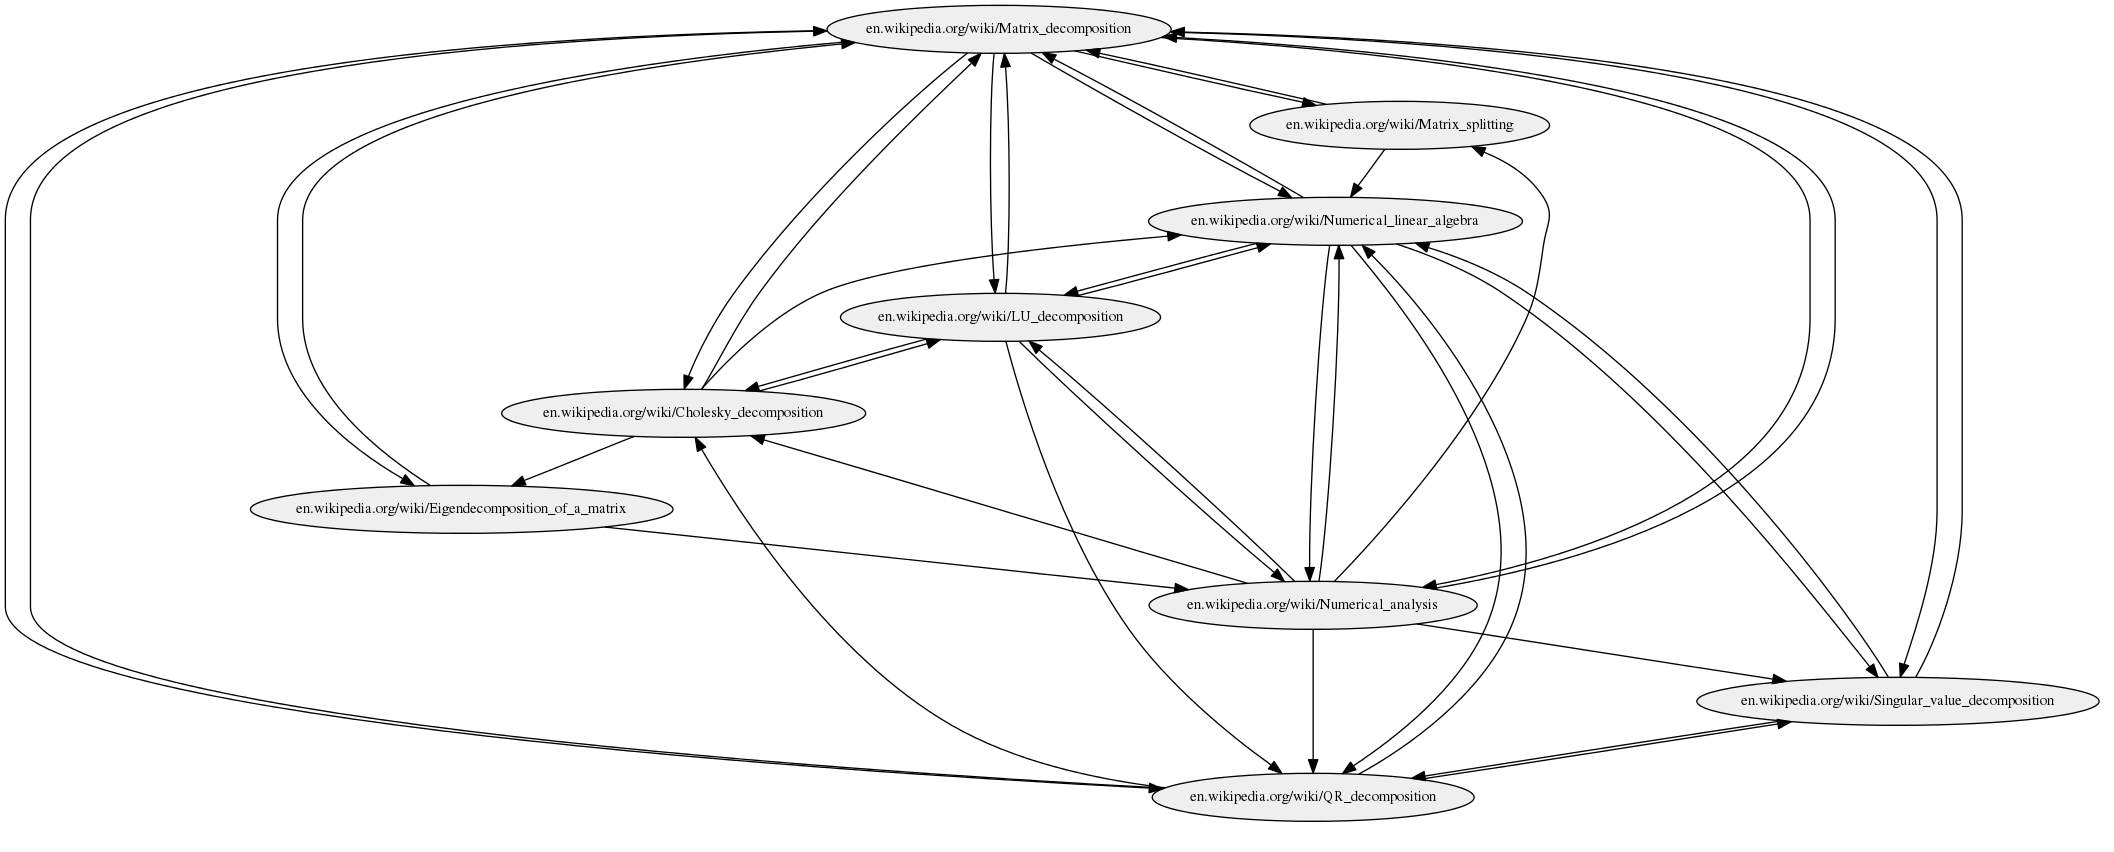
\includegraphics[width=0.75\textwidth]{exp2_conn_graph_metodos.png}
    \caption{Grafo de conectividad de p\'aginas de Wikipedia relacionadas con
        m\'etodos num\'ericos}
    \label{fig:wiki_graph}
\end{figure}

\par Sobre estas p\'aginas, calculamos los \'ordenes de PageRank e In-Deg, cuya
comparativa se encuentra detallada en el cuadro
\ref{tbl:pagerank_vs_indeg_wikipedia}. Nuevamente, In-Deg y PageRank dieron
resultados muy similares, pero no idénticos. M\'as aún, en In-Deg quedaron
varios nodos empatados, teniendo la misma cantidad de ejes entrantes. Pero esto
en PageRank no ocurri\'o, quedando definido un órden total.

\begin{table}[H]
    \centering
    \caption{\'Ordenes comparativos entre PageRank e In-Deg para Wikipedia}
    \label{tbl:pagerank_vs_indeg_wikipedia} 
    \setlength{\tabcolsep}{3pt}
    \begin{tabular}{|l|l||l|l|}
        \hline
        \multicolumn{2}{|c||}{PageRank} &\multicolumn{2}{c|}{In-Deg}\\
        \hline
        Puntaje & Nodo & Puntaje & Nodo\\
        \hline\hline
        0.196 & Matrix\_decomposition & 8 & Matrix\_decomposition\\
        0.165 & Numerical\_linear\_algebra & 7 & Numerical\_linear\_algebra\\
        0.125 & QR\_decomposition & 5 & QR\_decomposition\\
        0.106 & Numerical\_analysis & 4 & Numerical\_analysis\\
        0.105 & Singular\_value\_decomposition & 4 & LU\_decomposition\\
        0.098 & LU\_decomposition & 4 & Cholesky\_decomposition\\
        0.093 & Cholesky\_decomposition & 4 & Singular\_value\_decomposition\\
        0.057 & Eigendecomposition\_of\_a\_matrix & 2 & Eigendecomposition\_of\_a\_matrix\\
        0.050 & Matrix\_splitting & 2 & Matrix\_splitting\\
        \hline
    \end{tabular}
\end{table}

\par La diferencia entre \'ambos \'ordenes est\'a en la ubicaci\'on de
\emph{Singular value decomposition}. Mientras que en PageRank se encuentra en la
posici\'on 5, In-Deg lo lista en la 7ma ubicaci\'on. En el caso de In-Deg, la
determinaci\'on de la ubicaci\'on es determin\'istica, dependiendo del grado de
entrada del nodo que lo representa. Pero en nuestro ejemplo, vemos que existe un
empate con otros 3 nodos (como ya se ha explicado), con lo cual aqu\'i el orden
tambi\'en depende de la estabilidad y/o criterio de desempate que implemente
In-Deg. En nuestro caso, la implementaci\'on es estable, con lo cual se respeta
el orden inicial (o numeraci\'on) de los nodos. Por el otro lado, observando el
grafo podemos entender porque PageRank lo ubica en una posici\'on m\'as alta que
In-Deg: El nodo \emph{Numerical Linear Algebra}, uno de los de mayor puntaje (y
grado de entrada) tiene un link al nodo en cuesti\'on y a \emph{LU
decomposition}, pero no al resto de los valores que empatan en In-Deg. Por lo
visto en el experimento \ref{subsec:exp1}, sabemos que esto tiene un efecto de
subir el puntaje notoriamente en los nodos ''linkeados''. Luego, utilizando el
mismo razonamiento, observamos que \emph{Single value decomposition} queda por
encima de \emph{LU decomposition} por el voto/link de \emph{QR decomposition}.

\par Semánticamente, podemos observar que \textbf{en general}\footnote{\emph{QR}
queda por encima de \emph{Numerical Analysis}, creemos que esto se debe a la
morfología del grafo de referencias entre artículos en Wikipedia.} quedan
primeros en el ranking términos más \emph{generales} o \emph{abarcativos}; y a
medida que avanza el ranking se encuentran términos mas particulares.
Claramente, esta jerarqu\'ia de \emph{generalidad} es \'arbitraria para los
autores de este trabajo\footnote{¿Suma puntos hablar en tercera persona de
nosotros mismos? Very Scientific!}, aunque estimamos que habr\'a muy pocas
posibilidades de disenso al respecto para los temas representados por los nodos
del ejemplo.

\par Para evidenciar aún más la diferencia entre los algoritmos de In-Deg y
PageRank decidimos alterar expl\'icitamente el grafo de conectividad de este
\'ultimo ejemplo, agregando aristas desde los 5 nodos peor puntuados hacia uno
de los últimos en el ranking In-Deg (\emph{Eigendecomposition of a matrix}).
Esto deberia aumentar drásticamente el rankeo del ultimo elemento en In-Deg ya
que aumentamos su grado de entrada en 5, pero no tanto asi en Pagerank donde la
''calidad'' de los votantes tiene una mayor injerencia. Los resultados de este
último experimento pueden verse en el cuadro
\ref{tbl:pagerank_vs_indeg_wikipedia_modificado}. 

\begin{table}[H]
    \centering
    \caption{\'Ordenes comparativos entre PageRank e In-Deg para Wikipedia con grafo alterado explícitamente}
    \label{tbl:pagerank_vs_indeg_wikipedia_modificado}
    \setlength{\tabcolsep}{3pt}
    \begin{tabular}{|l|l||l|l|}
        \hline
        \multicolumn{2}{|c||}{PageRank} &\multicolumn{2}{c|}{In-Deg}\\
        \hline
        Puntaje & Nodo & Puntaje & Nodo\\
        \hline\hline
        0.189 & Matrix\_decomposition & 8 & Matrix\_decomposition\\
        0.137 & Numerical\_linear\_algebra & 7 & Numerical\_linear\_algebra\\
        0.123 & Numerical\_analysis & 7 & Eigendecomposition\_of\_a\_matrix\\
        0.114 & Eigendecomposition\_of\_a\_matrix & 5 & QR\_decomposition\\
        0.108 & QR\_decomposition & 4 & Numerical\_analysis\\
        0.097 & Singular\_value\_decomposition & 4 & LU\_decomposition\\
        0.089 & LU\_decomposition & 4 & Cholesky\_decomposition\\
        0.087 & Cholesky\_decomposition & 4 & Singular\_value\_decomposition\\
        0.051 & Matrix\_splitting & 2 & Matrix\_splitting\\
        \hline
    \end{tabular}
\end{table}

\par Puede observarse que respecto a In-Deg el elemento con ejes entrantes
artificiales paso a ser el
tercero por su nuevo grado de entrada aumentado. En Pagerank, el elemento subió
de ranking pero quedó por debajo de Numerical\_analysis, lo cual en principio es
raro, ya que este item quedó con puntaje 4 en In-Deg. Si miramos el grafo,
veremos que, efectivamente, el hecho de que \emph{Numerical analysis} sea apuntado por
\emph{Matrix decomposition} y \emph{Numerical linear algebra}, que son los términos mas
importantes, le da mas potencia al elemento en cuestión que al elemento
\emph{Eigendecomposition of a matrix}, apuntado por los últimos 5 de la lista.

%\par Por último, vemos que en el último experimento se acentúa el orden
%\texttt{abarcativo} de los resultados respecto al dominio de los elementos.

\medskip
\par A lo largo de este experimento pudimos evidenciar las diferencias que
existen entre dos algoritmos de elaboraci\'on de rankings distintos: In-Deg y
PageRank. Esto, que no lo hab\'iamos podido exponer en el experimento previo,
nos demostr\'o el peso que PageRank le otorga a los links provenientes de
p\'aginas web con mejores puntajes, diferenciaci\'on que In-Deg no realiza.
M\'as a\'un, nos encontramos conque In-Deg parece ser tener m\'as posibilidades
de empate en su forma de ''rankear'' que PageRank, volvi\'endose dependiente del
criterio de desempate que se utilice y convirti\'endose en otra
faceta/problema a resolver, situaci\'on que puede ser despreciada en el caso de
PageRank (las probabilidades de empate ya son chicas para pocos nodos, y las
mismas son cada vez menores a mayor cantidad). Como dato de color, observamos
que los resultados devueltos por \emph{Google} son bastante distintos de los
obtenidos con PageRank, con lo cual queda claro que a pesar de haber sido este
m\'etodo un hito en la historia del motor de b\'usqueda, el mismo ya a
evolucionado much\'isimo en pocos a\~nos, lo que demuestra la importancia del
problema estudiado. 


\newpage
\subsection{Convergencia de PageRank}
\label{subsec:exp3}
\begin{LaTeXdescription}
    \item[Objetivo] Estudiar como se comporta la convergencia en funci\'on de
        el factor de navegaci\'on $\alpha$.\\

    \item[Proposici\'on] PageRank propone una soluci\'on donde se observa a un
        conjunto de p\'aginas web como un grafo dirigido. Luego pasa este modelo
        a uno  matem\'atico, utilizando una matriz para computar una soluci\'on.
        Esta matriz, por construcci\'on, termina representando a un grafo
        completo (el grafo original no necesariamente lo era), y los valores del
        mismo dependen principalmente de 2 variables: $\epsilon$ y $\alpha$
        (algoritmo \ref{alg:power_method2}, p\'agina \pageref{alg:power_method2}
        y ecuaci\'on \ref{eq:M_def}, p\'agina \pageref{eq:M_def}). Si se observa
        el algoritmo, se ver\'a que claramente modificar el $\epsilon$ tendr\'a
        como resultado hacer que cada corrida converja en m\'as o menos
        iteraciones, ya que el criterio de parada depende de \'el. As\'i pues,
        no vemos como algo rico experimentar con este valor. En cambio, $\alpha$
        es una variable que modifica en gran medida a nuestra matriz $M$, con lo
        cual es dificil saber cual ser\'a su injerencia en la convergencia (en
        principio). El objetivo, entonces, es ver como $\alpha$ afecta al
        m\'etodo matem\'atico iterativo de la potencia en cuanto a su
        convergencia.\\

    \item[M\'etodo de Experimentaci\'on] Tomaremos 3 instancias de grafos de
        conectividad de p\'aginas web de tama\~no mediano-grande, obtenidas en
        \url{http://snap.stanford.edu/data/\#web}. Luego, correremos el
        algoritmo de PageRank para $\alpha=0.0$; $0.1$; $0.2$; $\dots$; $0.9$ y
        $\epsilon$ fijo en $0.00001$.\\

    \item[Resultados, an\'alisis y discusi\'on]
\end{LaTeXdescription}

\par En el gráfico \ref{subfig:exp3_comp} se exponen la cantidad de iteraciones
necesarias hasta converger a medida que el parámetro $\alpha$ crece. Para las 3
instancias el comportamiento observado es el mismo: a medida que el par\'ametro
$\alpha$ aumenta, la cantidad de iteraciones necesarias para converger crece
exponencialmente. Puede observarse que aunque con valores numéricos diferentes,
las curvas pertenecen a la misma familia de funciones, y por lo tanto tienen un
comportamiento id\'entico (emp\'iricamente hablando) en cuanto a la cantidad de
iteraciones en funci\'on de $\alpha$.

\begin{figure}[H]
    \centering
    \caption{An\'alisis de Convergencia en funci\'on de $\alpha$}
    \subfloat[][Iteraciones hasta Converger en funci\'on de $\alpha$]{
        \label{subfig:exp3_comp}
        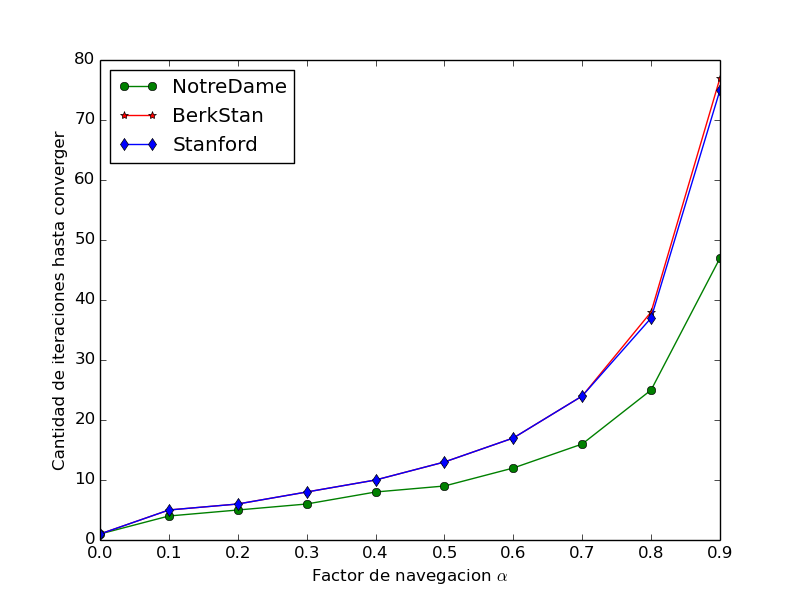
\includegraphics[width=.5\textwidth]{exp3_iteraciones_funcion_alpha.png}
    }
    \subfloat[][Velocidad de convergencia en funci\'on de $\alpha$\\Escala
    logar\'itmica]{
        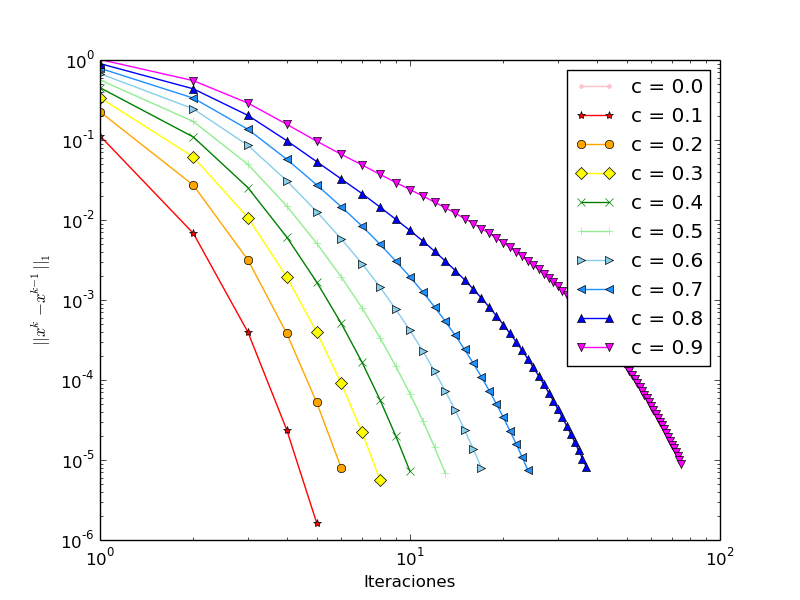
\includegraphics[width=.5\textwidth]{exp3_diff_funcion_iteraciones_standford.png}
        \label{subfig:exp3_diff}
    }
\end{figure}

\par Como se explic\'o en la secci\'on \ref{sec:introduccion}, el factor
$\alpha$ hace variar la proporci\'on entre $S$ y la matriz equiprobable a la
hora de definir a $M$. Es decir, en el rango de posibles valores de $\alpha$, la
\'unica manera en la que se afecta a $M$ es en los valores de cada uno de sus
elementos. Pero para ning\'un $\alpha$ se puede pasar a tener un elemento nulo
en $M$ (justamente se quer\'ia tener la representaci\'on de un digrafo
completo). As\'i pues, la pregunta pasa a ser: ¿Por qu\'e a mayor $\alpha$ se
necesitan m\'as iteraciones para converger?

\par Se nos ocurre que, volviendo al contexto de una cadena de Markov y el
navegante aleatorio, un $\alpha$ peque\~no nos genera una matriz de transici\'on
''m\'as'' equiprobable (recordar la definici\'on de $M$ en la ecuaci\'on
\ref{eq:M_def}, p\'agina \pageref{eq:M_def}) y dado que el método de la potencia
comienza inicialmente con el vector equiprobable, le toma pocas iteraciones
converger. A medida que $\alpha$ aumenta, el grafo generado denota más la
navegación estricta por los links entre los sitios, reduciendo la probabilidad
de teletransportación. Es decir, a mayor $\alpha$, el grafo se ''parece m\'as''
al grafo de conectividad original no adulterado (con los dangling nodes ya
resueltos), en el sentido de que $S$ predomina mucho m\'as en $M$ que
$(\rfrac{1}{n})ee^T$. Esta matriz $S$ no necesariamente representa un grafo
fuertemente conexo, una de las condiciones necesarias para asegurar convergencia
del método de la potencia en el contexto de este problema, con lo cual el método
de la potencia inicia sus iteraciones con una, si se quiere, \textbf{seguridad
de convergencia más débil}.

\par Respecto a la velocidad de convergencia, exponemos los resultados de una
sola instancia ya que para las 3 instancias los resultados son similares. Como
puede observarse en el gráfico \ref{subfig:exp3_diff}, a medida que el factor de
navegacion $\alpha$ crece, la velocidad de convergencia disminuye,
obteni\'endose curvas cada vez m\'as pronunciadas.

\par La ''velocidad de convergencia'' la definimos como la distancia
\emph{Manhattan} entre los autovectores $\vec{x^{(k)}}$ y $\vec{x^{(k-1)}}$
calculados en dos iteraciones consecutivas. Mientras mayor sea la distancia,
m\'as r\'apido decimos que se converge\footnote{Asumiendo que $\vec{x^{(k)}} <
\vec{x^{(k-1)}}$, caso contrario nos estar\'iamos alejando del criterio de corte
del m\'etodo, es decir, de converger.}, pues se est\'a acerc\'andose cada vez
\textbf{m\'as rápido} al umbral de corte del algoritmo (basado en $\epsilon$ o
una cantidad fija m\'axima de iteraciones\footnote{Esto se implementa, ya que si
bien la teor\'ia nos indica que el m\'etodo convergir\'a, los errores
n\'umericos de la aritm\'etica finita puede hacer que esto no ocurra.}).

\par Nuestra explicaci\'on para este comportamiento es exactamente la misma que
se expuso para el caso de las iteraciones hasta converger en funci\'on de
$\alpha$. Sin ir m\'as lejos, estamos hablando del mismo fen\'omeno, salvo que
en el caso de la figura \ref{subfig:exp3_diff} hacemos hincapi\'e en
\textbf{como} se acerca el m\'etodo al vector soluci\'on, mientras que en la figura
\ref{subfig:exp3_comp} observamos m\'as en detalle la \textbf{cantidad de
iteraciones} que se necesitan. Sin embargo, ambos gr\'aficos nos muestran lo
mismo: \textit{a que velocidad}, o \textit{cuanto tiempo/iteraciones} se
requieren para converger en funci\'on de $\alpha$.

\par Ahora bien, hemos visto como $\alpha$ afecta a la convergencia. S\'i esto
fuera lo \'unico, claramente siempre elegir\'iamos el valor que nos permita
converger m\'as r\'apido. Ocurre que, como vimos en el experimento
\ref{subsec:exp1}, el $\alpha$ afecta al orden obtenido tambi\'en, es decir, a
la calidad del resultado. As\'i pues, la elecci\'on de este par\'ametro ser\'a
la b\'usqueda del equilibrio \emph{efectividad} y \emph{eficiencia}, u entre
calidad del resultado y ti\'empo de c\'omputo (intuitivamente, m\'as iteraciones
implican mayor tiempo de c\'omputo). La bibliograf\'ia consultada nos indica que
en su momento, Google fij\'o inicialmente este par\'ametro en $0.85$,
considerando a este un \emph{trade-off} lo suficientemente
bueno\cite{Bryan2006}\cite{Langville2006}.

\par As\'i pues conclu\'imos nuestra experimentaci\'on sobre la convergencia del
m\'etodo de la potencia para PageRank. Llegamos a un resultado inmediato que nos
dice que a mayor $\alpha$ tendremos una velocidad de convergencia menor y, ergo,
una cantidad de iteraciones necesaria mayor para obtener un resultado lo
suficientemente apr\'oximado. Tambi\'en evaluamos brevemente la contracara de
tener un tiempo de convergencia chico: el resultado obtenido no necesariamente
es el mismo ya que predomina m\'as la equiprobabilidad de los ejes de
teletransportaci\'on artificalmente a\~nadidos a la matr\'iz $M$. Tambi\'en
obtuvimos como resultado que este comportamiento es, presumiblemente (har\'ia un
falta un an\'alisis m\'as minucioso para poder afirmarlo), el mismo para
cualquier instancia de entrada, m\'as all\'a de que la cantidad de iteraciones
absoluta entre dos instancias pueda variar para el mismo $\alpha$, el
comportamiento en funci\'on de $\alpha$ parecer\'ia ser el mismo.


\newpage
\subsection{An\'alisis de Tiempo de C\'omputo}
\label{subsec:exp4}
\begin{LaTeXdescription}
    \item[Objetivo] Analizar la complejidad temporal del m\'etodo.\\

    \item[Hip\'otesis] Proponemos que el tiempo de c\'omputo por iteraci\'on
        para una instancia y $\epsilon$ fijos ser\'a siempre el mismo para todo
        $\alpha$. Tambi\'en proponemos que el tiempo de c\'omputo por interación
        para $\epsilon$ fijo ser\'a el mismo para \textbf{toda instancia} (sin
        importar tama\~no, cantidad de ejes, etc).\\

    \item[Proposici\'on] De los experimentos previo hemos llegado a la
        conclusi\'on de que a mayor $\alpha$, mayor cantidad de iteraciones
        ser\'an necesarias para converger, lo cual implica inmediatamente un
        mayor tiempo de c\'omputo requerido. La pregunta ideal a responder
        ser\'ia ''cu\'anto tiempo'', pero tambi\'en concluimos previamente que
        la cantidad de iteraciones es dependiente (entre otros factores) de la
        instancia de entrada. Con lo cual, responder a esta pregunta en el
        contexto de este trabajo es imposible sin una cota te\'orica para la
        cantidad de iteraciones (que ni siquiera sabemos si existe). En cambio,
        lo que s\'i podemos analizar es si el tiempo de c\'omputo \textbf{por
        iteraci\'on} es el mismo para toda instancia, sin importar el
        $\epsilon$\footnote{M\'as all\'a de para nuestros experimentos lo
        estemos dejando fijo.} o $\alpha$. Analizamos entonces si el tiempo por
        iteraci\'on var\'ia seg\'un la densidad de la instancia inicial, y a su
        vez si varía para distintos valores de $\alpha$.\\

    \item[M\'etodo de Experimentaci\'on] Tomamos 3 instancias de tama\~no
        mediano-grande, con una diferencia relativa de densidad entre ellas
        significativa. Particularmente, tomamos las mismas del experimento
        anterior. Luego resolvemos cada instancia con PageRank 10 veces para
        $\alpha=0.0$; $0.1$; $0.2$; $\dots$; $0.9$\footnote{Totalizando un total
        de 300 corridas del m\'etodo (10 corridas para 10 valores de $\alpha$
        para 3 instancias distintas).}. Tomamos entonces para cada instancia y
        $\alpha$ fijos, el promedio de los tiempos de c\'omputo. Por \'ultimo,
        calculamos el tiempo de c\'omputo por iteraci\'on dividiendo este
        promedio por la cantidad de iteraciones totales que necesit\'o el
        m\'etodo para converger.\\

    \item[Resultados, an\'alisis y discusi\'on]
\end{LaTeXdescription}

\par Consideramos 2 enfoques para extraer conclusiones, el primero analiza el
tiempo consumido por iteración por el método de la potencia para diferentes
valores de $\alpha$ y el segundo se centra en el tiempo por iteraci\'on respecto
de la densidad de la instancia/grafo de entrada\footnote{Al referirnos a
\emph{densidad} de un grafo, nos referimos a la cantidad de ejes que tiene. A
mayor cantidad de ejes, m\'as denso es.}.

\begin{figure}[H]
    \centering
    \caption{An\'alisis de Tiempo de C\'omputo} %en funci\'on de $\alpha$}
    \subfloat[][Tiempo por Iteraci\'on en funci\'on de $\alpha$.]{
        \label{subfig:exp4_tiempo_iteracion}
        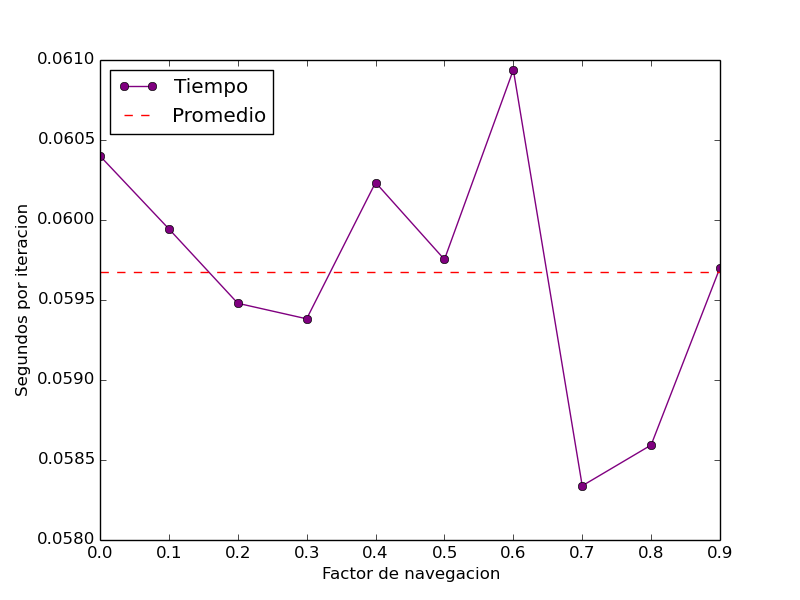
\includegraphics[width=.55\textwidth]{exp4_tiempo_por_iteracion_notredame.png}
    }
    %\begin{figure}[H]
    %    \centering
        \subfloat[][Tiempo por Iteraci\'on promedio vs Densidad del Grafo]{
            \label{subfig:exp4_den}
            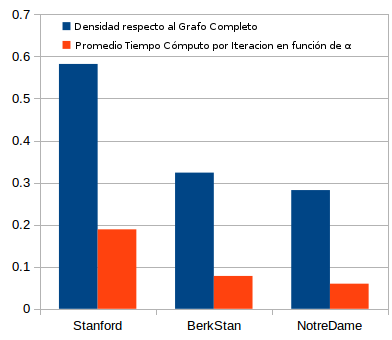
\includegraphics[width=.45\textwidth]{exp4_tiempo_vs_densidad.png}
        }
        %\caption{An\'alisis de Tiempo de C\'omputo en funci\'on de la densidad del Grafo}
    %\end{figure}
    %\subfloat[][Tiempo por Iteraci\'on en funci\'on de $\alpha$. Escala logarítmica]{
    %    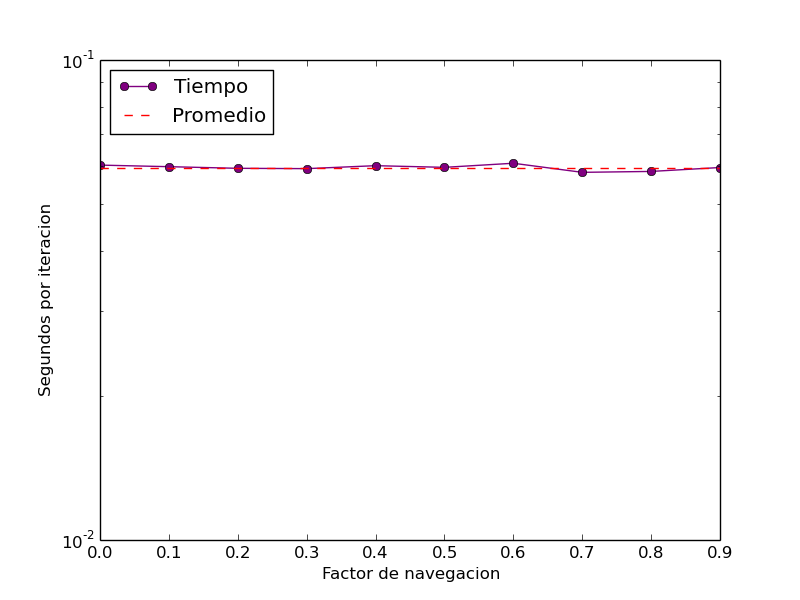
\includegraphics[width=.45\textwidth]{exp4_tiempo_por_iteracion_notredame_log.png}
    %    \label{subfig:exp4_tiempo_iteracion_log}
    %}
\end{figure}

\par Para el primer enfoque, observemos los resultados obtenidos en la figura
\ref{subfig:exp4_tiempo_iteracion}. En el mismo observamos dos curvas. La
primera, \emph{Tiempo}, que representa el tiempo por iteraci\'on promedio para
cada $\alpha$ (calculado como el tiempo promedio hasta converger de las 10
ejecuciones para un $\alpha$ fijo, dividido por la cantidad de iteraciones que
necesit\'o); y la segunda \emph{Promedio} que no es otra cosa que el promedio de
los tiempos por iteraci\'on calculados para la curva \emph{Tiempo}. Los
resultados expuestos en esta figura son similares para las 3 instancias de
prueba que se tomaron, con lo cual se decidi\'o exponer una sola.

\par Puede observarse en esta misma figura que el tiempo por iteraci\'on
calculado en funci\'on de $\alpha$ oscila en valores muy pequeños alrededor del
promedio. Para ilustrar esto, presentamos en el cuadro
\ref{tbl:exp4_data_notredame} las m\'etricas empíricas del experimento.

\begin{table}[H]
    \centering
    \caption{Métricas del tiempo por iteracion respecto de $\alpha$}
    \label{tbl:exp4_data_notredame} 
    \setlength{\tabcolsep}{3pt}
    \begin{tabular}{|l|l|}
        \hline
        Métrica & Segs\\
        \hline\hline
        Promedio & 0.059676\\
        Desv\'io Est\'andar & 0.000788\\
        M\'inimo & 0.058338\\
        M\'aximo & 0.060938\\
        Diferencia \%\footnotemark& 4.266231\\
        \hline
    \end{tabular}
\end{table}
\footnotetext{Diferencia \%: 100*(max-min)/max.}


\par Estas variaciones seguramente se deben al \emph{scheduler} del sistema
operativo y a fenómenos de bajo nivel de las corridas de los
experimentos. De hecho, ya vimos en el experimento \ref{subsec:exp3} que a
medida que aumentamos el $\alpha$, m\'as iteraciones ser\'an necesarias para
converger. Obviamente esto implica un mayor tiempo de c\'omputo, ergo, la
ejecuci\'on del experimento se vuelve a\'un m\'as sensible pues al estar m\'as
tiempo ejecut\'andose m\'as probabilidades hay de que el Sistema Operativo
decida darle el CPU a otro proceso de mayor prioridad que surja (o que al estar
tanto tiempo ejecut\'andose, su prioridad vaya bajando).

\par Finalmente conclu\'imos que que el tiempo por iteraci\'on es constante, ya
que en las m\'etricas nos confirman, al observar los valores muy peque\~nos del
desv\'io est\'andard y diferencia porcentual, que estas diferencias para
distintos $\alpha$ sean muy probablemente errores de medici\'on (recordemos que
adem\'as estamos trabajando con instancias de entrada de tama\~no
mediano-grande).

\par Habiendo llegado a la conclusi\'on que la hip\'otesis sobre el tiempo de
c\'omputo por iteraci\'on es constante, debemos analizar por qu\'e. Repasando la
secci\'on \ref{sec:implementacion}, podemos decir que es razonable el
comportamiento presupuesto y observado, ya que el valor de $\alpha$ no modifica
la \emph{densidad} de la matriz original de conectividad $A$. Recordemos
entonces que nuestra implementaci\'on se basa en el algoritmo
\ref{alg:power_method3}, p\'agina \pageref{alg:power_method3}, que multiplica
usando justamente esta matriz $A$ y aprovechando que la misma es esparsa. Al no
modificar esta caracter\'istica la selecci\'on del par\'ametro $\alpha$, podemos
afirmar que la cantidad de $flops$ necesarios para el producto matriz-vector se
mantendr\'a constante en funci\'on de $\alpha$ (de hecho, $\alpha$ es un
par\'ametro que luego multiplica al vector resultante $A\vec{x}^{(k-1)}$ en
nuestro algoritmo, con lo cual no afecta en lo absoluto al producto
matriz-vector que involucra a $A$).

\par El segundo enfoque centra su atención en el tiempo por
iteracion respecto a la densidad del grafo asociado a la instancia de entrada.
Al contrario que lo esperado, la densidad (cantidad de ejes) del
grafo \textbf{s\'i} altera el tiempo de cómputo por iteración. Si observamos la
figura \ref{subfig:exp4_den}, observaremos que a mayor densidad, mayor tiempo
por iteraci\'on se necesita.

\par En esta figura se compara el tiempo promedio consumido\footnote{Se utiliza
el valor promedio del tiempo para todos los factores de navegación.} contra una
medida de densidad del grafo\footnote{Se toma como métrica un cociente entre la
cantidad de aristas del gráfo y la cantidad de aristas de una \emph{clique} de
su misma cantidad de nodos; multiplicado por una constante para igualar las
magnitudes con los valores de los tiempos de c\'omputo.}, y se v\'e, para las 3
instancias evaluadas, que el crecimiento del tiempo de c\'omputo parecer\'ia ser
l\'ineal en funci\'onde la densidad del grafo. Dado que s\'olo experimentamos
con estas 3 instancias, ser\'ia muy abrupto hacer dicha afirmaci\'on, pero si
podemos decir que tenemos sospechas de que eso ocurra, dejando este aspecto para
un futuro posible experimento\footnote{Vale la pena aclarar, en este caso, que
podr\'iamos considerar a nuestras 3 instancias como poco densas, m\'as alla de
la diferencia notoria de densidad entre ellas.}.

\par Volviendo al hecho de que a mayor densidad, mayor ti\'empo de c\'omputo,
llegamos a la conclusi\'on de que esto se debe al mismo motivo que en el primer
enfoque, salvo que esta vez justifica el hecho de que \textbf{s\'i} se requiera
m\'as tiempo de c\'omputo. Ocurre que al ser la instancia de entrada m\'as
densa, menos esparsa ser\'a $A$ (m\'as ejes implica mayor cantidad de valores no
nulos en la matriz), y por lo tanto el producto $A\vec{x}$ de la
implementaci\'on del m\'etodo efectuar\'a m\'as $flops$.

\medskip
\par Finalizando, concluimos que 1 de nuestras hip\'otesis era correcta, y la
otra no. Peculiar es, que las justificaciones que le encontramos a ambos
comportamientos (la relaci\'on tiempo de c\'omputo por iteraci\'on en funci\'on
de $\alpha$ y de la densidad de la instancia) es la misma: mientras que $\alpha$
no afecta a la densidad de la matriz de conectividad pesada $A$, cosa que si lo
hace la cantidad de ejes del grafo. Es decir, terminamos entendiendo que el
principal aspecto a tener en cuenta a la hora de ver como se ver\'a afectado el
tiempo de computo (para nuestra implementaci\'on basada en el algoritmo
propuesto por Kamvar et al.\cite{Kamvar2003}) ser\'a la
densidad/esparcidad\footnote{Coloquialismo.} de la matriz inicial del modelo.


\newpage
\subsubsection{PageRank/GeM vs Orden Total Conocido}
\label{subsec:exp5}
\begin{LaTeXdescription}
    \item[Objetivo] Analizar la convergencia del modelo GeM asumiendo que
        existe ranking ideal y correcto al cual converger.\\

    \item[Hip\'otesis] PageRank, utilizando el modelo GeM, converge finalmente a
        un ''Orden Real'' o ''Correcto'' de los competidores deportivos, si este existe.
        Adem\'as, no necesitar\'a de un grafo completo (los resultados de todos
        contra todos) para converger al mismo.\\

    \item[Proposici\'on] Como se coment\'o previamente en la experimentaci\'on
        sobre p\'aginas web, establecer cuál es el ''mejor orden'' u ''orden
        correcto'' es completamente arbitrario. No hay una vara sobre la cual
        medir. En los deportes esto es a\'un más evidente, ya que depende de
        los resultados deportivos, ¿y qui\'en es capaz de afirmar que la
        probabilidad de que Platense -el mejor equipo del mundo e insipirador
        del t\'itulo del enunciado de este trabajo- le gane al Barcelona es $0$?
        As\'i pues, en el caso de los deportes tampoco tenemos un orden total,
        conocido y determin\'istico para verificar que el resultado de PageRank
        es el correcto. Pero si existiese este orden, si fuese determin\'istico,
        ¿PageRank convergir\'ia al mismo?\\

    \item[M\'etodo de Experimentaci\'on] Generamos dos instancias ideales y
        completamente abstractas de los resultados de un torneo de f\'utbol con
        10 y 50 equipos respectivamente, que juegan todos contra todos una
        \'unica vez (45 partidos para la primera instancia, 1225 para la
        segunda). Las instancias son construidas de manera tal que $equipo_i$ le
        gana a $equipo_j$ si y s\'olo si $i<j$. Es decir, el ranking correcto es
        la numeraci\'on de los equipos de forma ascendente, y cada $equipo_i$
        ocupa el puesto $i$.

        \par Aprovechamos el hecho de que en los deportes hay una componente
        temporal y generamos los partidos por fecha (es decir, grupos de
        partidos que ocurren todos al mismo tiempo, o al menos as\'i ser\'a para
        la perspectiva del algoritmo, que recibir\'a todos los partidos de una
        fecha juntos). En cada fecha se enfrentan, de a dos, equipos que no se
        hayan enfrentado todav\'ia y que no jueguen otro partido esa misma
        fecha. Dentro de esas restricciones, los enfrentamientos de cada fecha
        se eligen al azar, pero con una semilla fija (5) para obtener
        reproducibilidad en los experimentos. \textbf{Notar que la cantidad de
        fechas necesarias para que se jueguen todos los partidos no est\'a
        determinada \'unicamente por la cantidad de equipos sino que depende
        tambi\'en de como se elijan los enfrentamientos de cada fecha. Esto se
        debe a que confeccionar un generador de instancias aleatorias que
        respete las restricciones y genere un fixture de $n-1$ equipos es
        complejo y escapa a los objetivos de este trabajo. As\'i pues, nuestra
        instancia de 10 equipos \underline{consta de 11 fechas} y la instancia
        de 50 equipos \underline{consta de 53 fechas}}.

        \par El resultado de todos los partidos es siempre 1 a 0. No hace falta
        considerar empates dado que siempre hay un ganador.
        
        \par Ejecutamos
        GeM tantas veces como fechas haya, pas\'andole en cada instancia una
        fecha m\'as. Es decir, en la ejecuci\'on 1 le pasamos los resultados de
        la fecha 1, en la 2 los resultados de la fecha 1 y 2, y as\'i
        sucesivamente. Para cada resultado de GeM, comparamos el ranking
        obtenido con el correcto, para alguna medida de distancia entre
        rankings, que definiremos m\'as adelante.

        \par Hace falta considerar un detalle importante, que es qu\'e
        decisi\'on tomar ante empates del ''puntaje'' asignado por GeM. Si
        desempat\'aramos por n\'umero de equipo de manera ascendente caer\'iamos
        en el molesto caso de que ya desde antes de empezar el torneo la salida
        de GeM coincidir\'ia con el orden ideal. Lo mismo vale para cualquier
        subconjunto de competidores empatados en un momento dado: su orden
        relativo coincidir\'ia con el ideal, aunque por casualidad y no por
        virtud del algoritmo. Resolvimos entonces ''romper'' el caso y que el
        desempate se realice de manera descendente, asegur\'andonos as\'i de no
        evaluar como correctos resultados en donde hay muchos empates.

        \par Repetimos el experimento variando los valores de $\alpha$ en
        factores de $0.2$, para estudiar la convergencia en cada caso.  De
        confirmarse nuestra hip\'otesis la diferencia/distancia del ranking
        respecto del orden total ideal (que sabemos que existe por
        construcci\'on) deber\'ia llegar a ser 0, eventualmente ''antes'' de que
        se hayan jugado todas las fechas.\\

    \item[Resultados, an\'alisis y discusi\'on]
\end{LaTeXdescription}

\par En primer lugar, como hemos adelantado, debemos decidir cómo determinar la
''distancia'' entre dos rankings. Es decir, determinar alguna manera de comparar
dos rankings dados, y poder tener una magnitud de cuan parecidos son. Para ello
consideramos algunas opciones dados dos rankings A y B, de entre las cuales
mencionamos:

\begin{enumerate}
        \item La sumatoria de la distancia, para cada competidor, entre su
            posici\'on en el ranking A y la posici\'on en el ranking
            B.\label{itm:distancia_rankings}
        \item La cantidad de competidores que aparecen, en A, en una posición distinta a la que aparecen en B.
        \item La sumatoria, para cada competidor, de la cantidad de equipos que tiene por encima en A y que tiene por debajo en B.
\end{enumerate}

\par Luego de evaluar estas opciones (y algunas m\'as no tan concisas),
decidimos trabajar de aqu\'i en m\'as con la distancia basada en la suma de las
distancias de todos los competidores (definici\'on de distancia n\'umero
\ref{itm:distancia_rankings}). Consideramos que dicha forma de tomar la
distancia entre dos rankings, de alguna manera nos est\'a se\~nalando cuántas
permutaciones de elementos/equipos contiguos hay entre un ranking y el otro,
cosa que no queda tan claro con las dem\'as opciones. Y esa forma de medir la
distancia es la que consideramos que se ajusta a lo que queremos observar del
dominio del problema: cu\'antos equipos est\'an ubicados distinto y cuán lejos.

\begin{figure}[H]
    \caption{Distancia al orden total ideal/correcto ($c = \alpha$)}
    \label{fig:exp5_1}
    \centering
    \subfloat[][Torneo de 10 equipos]{
        \label{subfig:exp5_10equipos}
        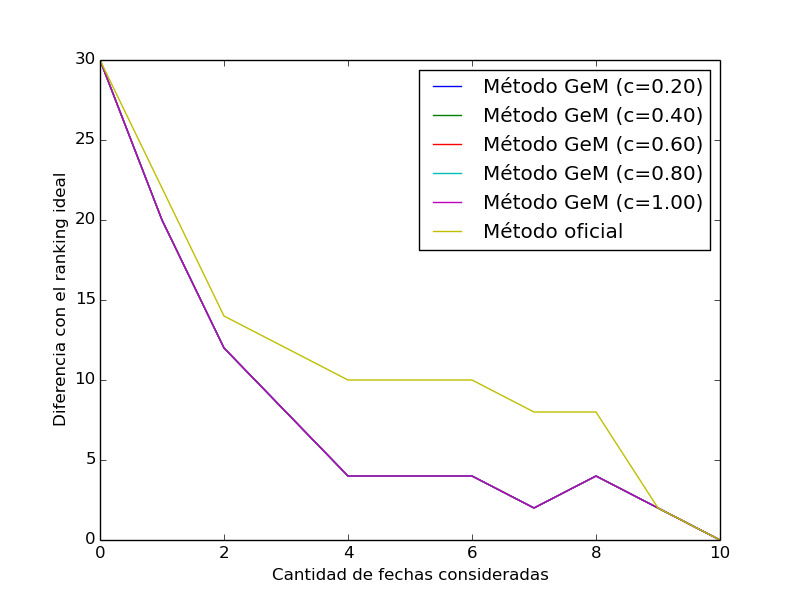
\includegraphics[width=.5\textwidth]{exp5_10_equipos.png}
    }
    \subfloat[][Torneo de 50 equipos]{
        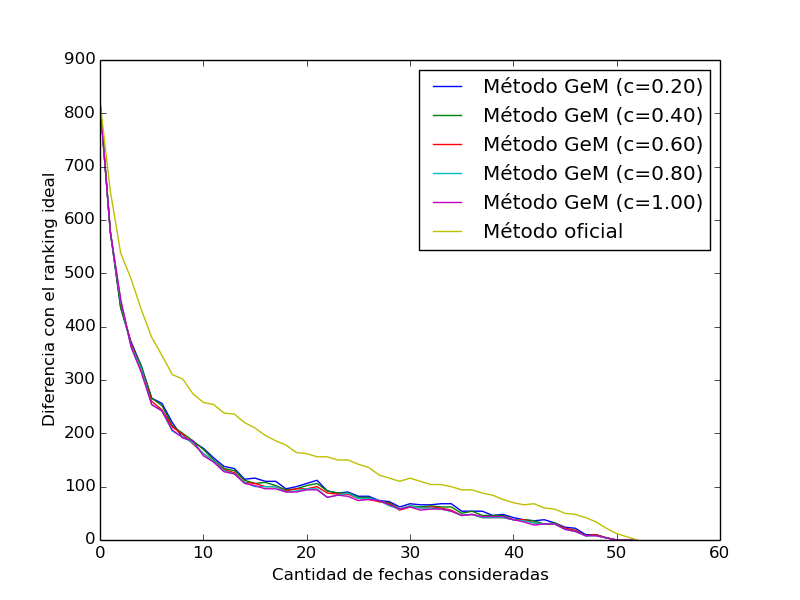
\includegraphics[width=.5\textwidth]{exp5_50_equipos.png}
        \label{subfig:exp5_50equipos}
    }
\end{figure}

\par La hip\'otesis fue confirmada. GeM converge al Orden Real para todos los
valores no nulos de $\alpha$ y no precisa todas las fechas para hacerlo, como se
puede observar en la figura \ref{fig:exp5_1}. Sin embargo, necesita una cantidad
significativa: para todos los valores no nulos de $\alpha$ fueron necesarias 10
de 11 fechas para el caso de 10 equipos y 50 de 53 fechas para el caso de 50
equipos.

\par El caso $\alpha=0$ no funciona porque la matriz termina descartando los
resultados de los equipos y usando simplemente la misma probabilidad para
cualquier equipo. En adelante dejaremos de lado este caso.

\par La variaci\'on $\alpha$ en el caso de 10 equipos no represent\'o
diferencias en el orden devuelto en cada fecha. es por eso que en la figura
\ref{subfig:exp5_10equipos} no se ven m\'as que dos curvas (una de las cuales
corresponde al siguiente experimento): estan todas superpuestas. En el caso de
50 equipos s\'i hubo leves diferencias en el orden devuelto en cada fecha.
Observamos que a mayor $\alpha$ el algoritmo en general converge ''mejor'' al
Orden Real (es decir, dada la misma cantidad de fechas, se acerca m\'as), aunque
siempre precisa 50 fechas para converger al orden real (figura
\ref{subfig:exp5_50equipos}). La diferencia de todos modos es peque\~na y probablemente se deba a que, en
nuestro modelo ideal, las victorias son totalmente transitivas: la probabilidad
de que $C$ le gane a $A$ dado que $A$ le gan\'o a $B$ y $B$ le ganó a $C$ es
siempre $0$.  Como valores peque\~nos de $\alpha$ tienden a agregar una
probabilidad de que $C$ efectivamente le gane a $A$, la convergencia mejora
levemente para valores altos de $\alpha$ (donde esa probabilidad artificial es
cada vez menor). Sin embargo, variando la semilla usada para ordenar los
enfrentamientos encontramos casos en donde un valor mayor de $\alpha$ empeoraba
la convergencia en alg\'un punto (ver figura \ref{subfig:exp5_c_malo}), por lo
que no podemos generalizar esta conclusi\'on.

\par As\'i pues, motivados por estos resultados, realizamos la siguiente
experimentaci\'on.

%---------------------------------------------------------------
\subsubsection*{PageRank vs Ranking FIFA en un caso de Orden Total Conocido}
\label{subsec:exp5_aux}
\begin{LaTeXdescription}
    \item[Objetivo] Comparar GeM contra el raking est\'andar del f\'utbol en un
        caso ideal.\\

    \item[Hip\'otesis] PageRank, utilizando el modelo GeM, converge m\'as
        r\'apido al ''Orden Real'', si lo hay, que el sistema oficial del
        f\'utbol asociado establecido por la FIFA\cite{fifa}.\\

    \item[Proposici\'on] Asumiendo que se confirm\'o la hip\'otesis del
        experimento anterior, nos interesa analizar si, asumiendo que existe un
        orden ideal/correcto, GeM se comporta peor, igual o mejor que la forma
        est\'andar de ordenar a los equipos (por puntos, 3/1/0 puntos para
        victoria/empate/derrota) donde ''comportarse'' mejor significa que con
        la misma información disponible (por ejemplo, la mitad de los partidos
        jugados) se acerca m\'as al orden ideal.\\

    \item[M\'etodo de Experimentaci\'on] Consideramos las mismas instancias de
        prueba que el experimento anterior. Comparamos la distancia entre GeM y
        el orden ideal contra la distancia entre el ordenamiento est\'andar y el
        orden ideal, usando la misma definici\'on de distancia de rankings que
        para el experimento anterior y el mismo criterio para ordenar equipos
        empatados en puntaje. De confirmarse nuestra hip\'otesis, deber\'iamos
        ver que GeM se acerca ''m\'as r\'apido'', es decir, con menos fechas, al
        orden ideal.\\

    \item[Resultados, an\'alisis y discusi\'on] 
\end{LaTeXdescription}

\begin{figure}[H]
    \caption{Casos Patol\'ogicos (10 equipos, $c = \alpha$)}
    \label{fig:exp5_2}
    \centering
    \subfloat[][Caso particular malo para $\alpha$ grande]{
        \label{subfig:exp5_c_malo}
        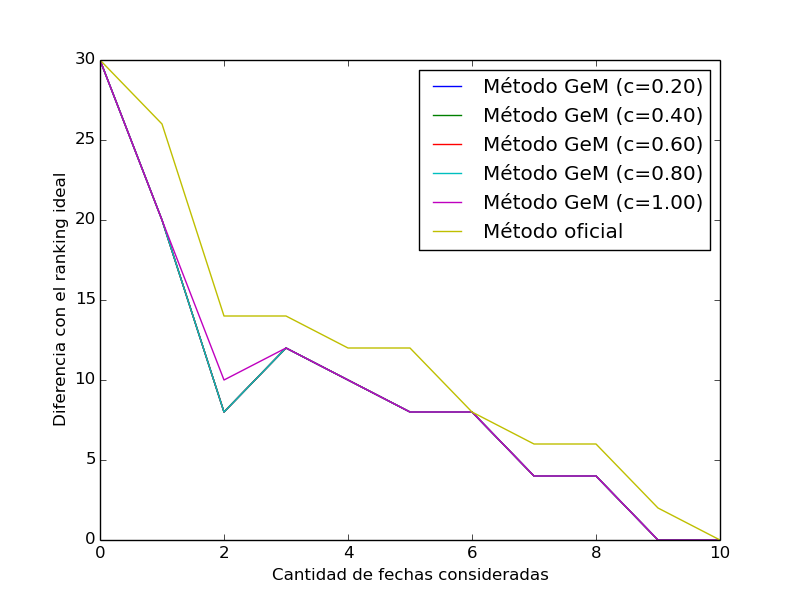
\includegraphics[width=.5\textwidth]{exp5_ejemplo_c_malo.png}
    }
    \subfloat[][Caso particular malo para GeM]{
        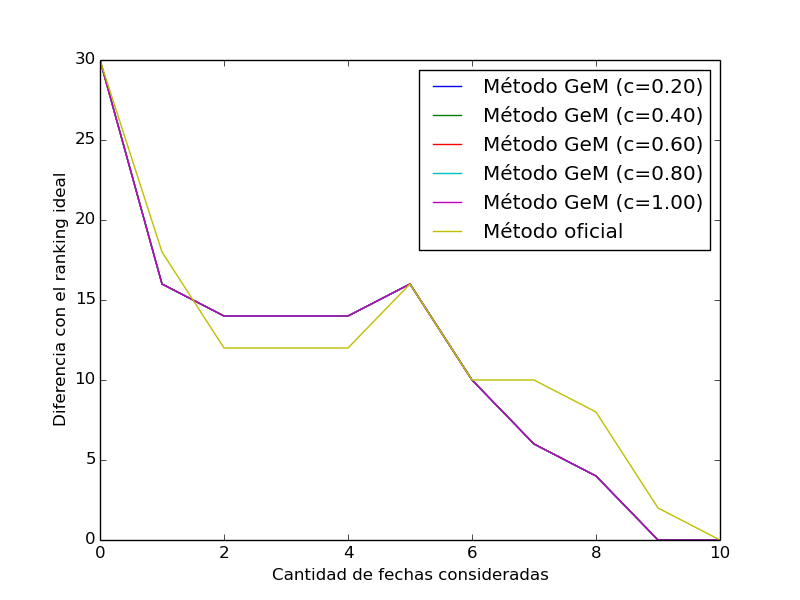
\includegraphics[width=.5\textwidth]{exp5_ejemplo_gem_malo.png}
        \label{subfig:exp5_gem_malo}
    }
\end{figure}

\par Comparamos GeM con el orden oficial, establecido por asignación de puntos
(3-1-0) y confirmamos tambi\'en nuestra hip\'otesis de que en el caso promedio,
GeM se comporta mejor que el orden oficial de asignaci\'on de puntajes,
acerc\'andose más al ideal para cualquier cantidad de fechas.

\par Sin embargo tambi\'en encontramos semillas para las cuales esto no era real
en alg\'un punto (ver figura \ref{subfig:exp5_gem_malo}) por lo que tampoco
podemos generalizar esta conclusi\'on.

\par Por \'ultimo, dado que los dos casos ''patol\'ogicos'' fueron encontrados
con la instancia de pocos equipos (10) y no logramos encontrar una semilla que
los genere en el caso de muchos (50), podr\'iamos argumentar que GeM se comporta
''mejor'' cuando la cantidad de equipos es grande. Queda fuera de los alcances
de este trabajo confirmar m\'as sistem\'aticamente esa hip\'otesis, pero es un
buen trabajo futuro.

%---------------------------------------------------------------
\medskip
\par En este experimento se trabaj\'o principalmente con instancias artificiales
''de juguete''. Las mismas lejos est\'an de representar la realidad, pero nos
sirvieron para poder asegurar que el modelo GeM ''descubrir\'ia'' el ranking
justo (o real, como dir\'ia Platon) si este existiese. A\'un as\'i, observamos
que para llegar a este ranking el modelo requerir\'a de mucha informaci\'on de
entrada, lo cual le quita quiz\'as utilidad como predictor de resultados de
torneos\footnote{Sin \'animo de menospreciar a GeM, si uno tiene los datos de 50
sobre 53 fechas, predecir con buena probabilidad de acierto el orden final no es
necesariamente una tarea extremadamente dif\'icil.}. Tambi\'en observamos que en
la progesi\'on fecha a fecha, el par\'ametro $\alpha$ pareciera tener de muy
poca a nula influencia sobre los rankings obtenidos.

\par Por \'ultimo, al comparar la ''velocidad de aproximaci\'on al ranking ideal'' con el sistema de puntaje real, pudimos ver que si
bien considerabamos no tan bueno a GeM para aproximarse con poca informaci\'on
al resultado final, se comporta mejor que el ranking oficial (para
los casos ideales que fueron considerados), con lo cual este modelo quiz\'as
podr\'ia ser un primer paso hacia un predictor de resultados de torneos de
f\'utbol profesional\footnote{Y la dominaci\'on mundial.}.


\newpage
\subsubsection{GeM vs Ranking Oficial}
\label{subsec:exp6}
\begin{LaTeXdescription}
    \item[Objetivo] Comparar GeM con los rankings estándar en el mundo real.\\

    \item[Proposici\'on] En la vida real la emoción subyacente de los deportes
        radica, en parte, en la posibilidad de que cualquiera le gane a
        cualquiera. ¿Para qué practicar u observar/seguir un deporte si este no
        es el caso?  Un ranking trata de dar un orden que determine que
        participante es mejor que otro entre los que forman parte de una
        competición. Pero la confección de este ranking puede tener que variar
        de acuerdo a la forma de la competición: no en todos los eventos todos
        los equipos juegan contra todos, no siempre todos juegan la misma
        cantidad de partidos ni la misma cantidad de veces entre sí. Así pues,
        dar un ranking se vuelve más complicado. Nuestra idea es tomar casos del
        mundo real y observar los resultados de GeM y ver cómo se comporta
        respecto de estas asimetrías inherentes al tipo de competición; mientras
        que lo comparamos contra el ranking oficial utilizado en cada caso.\\

    \item[M\'etodo de Experimentaci\'on] Evaluaremos 3 instancias de
        deportes/ligas:

        \begin{enumerate}
            \item El campeonato de Primera División del fútbol argentino 2015,
                tomando hasta la fecha 23.

            \item La Copa Mundial de la FIFA de 2014, realizada en Brasil.

            \item La Copa Mundial de la FIFA de 1954, realizada en Suiza.
        \end{enumerate}
        \medskip

        \par Tomamos el campeonato argentino como un ejemplo del formato de
        liga, y las Copas Mundiales de Fútbol como un ejemplo del caso en que no
        juegan todos contra todos ni todos juegan la misma cantidad de veces.
        Tomamos el caso de 2014 como representante del formato ''actual'' de 32
        equipos con una única fase de grupos y una fase eliminatoria. Y tomamos
        el caso de 1954 por presentar una situación interesante de analizar: en
        la fase de grupos Hungría le ganó 8 a 3 al que luego saldría campeón,
        Alemania Federal.

        \par Para los casos de los Mundiales, tomamos como ''oficial'' el
        ranking final publicado por la FIFA. Para el caso del campeonato de
        primera división, la ordenación estándar por puntaje 3-1-0.

        \par En los tres casos ejecutamos el algoritmo GeM variando los valores
        de $\alpha$ y comparamos contra el ranking oficial de la instancia. En
        los tres casos decidimos ignorar los empates. Para las definiciones por
        tanda de penales, tomamos como resultado del partido el resultado final
        de los mismos.\\

    \item[Resultados, an\'alisis y discusi\'on]
\end{LaTeXdescription}

%%*************************************************************************
\begin{enumerate}[parsep=1ex]
    \item Lo primero que notamos es que para valores grandes de $\alpha$ la
        diferencia con el ranking oficial aumenta, alcanzando un mínimo en
        $\alpha=0.1$. Consideramos que esto tiene que ver por darle demasiada
        importancia a la ''transitividad de victorias'' cuando el fútbol en
        general no funciona de esa manera. Por ejemplo, para $\alpha=1$ los
        primeros cinco puestos son:

        \begin{figure}[H]
            \centering
            \subfloat[][Primeros Puestos\label{subfig:exp6_arg}]{
                \footnotesize
                \setlength{\tabcolsep}{3pt}
                \begin{tabular}[b]{|l|r||l|r|}
                    \hline
                    \multicolumn{2}{|c||}{GeM}&\multicolumn{2}{c|}{Oficial: 3-1-0}\\
                    \hline
                    Equipo & Puntaje & Equipo & Puntaje\\
                    \hline\hline
                    Boca Juniors &0.0934262& San Lorenzo &50 \\
                    River Plate &0.0828491& Boca Juniors &49 \\
                    San Martín (SJ) &0.0674819& Racing Club &46 \\
                    Aldosivi &0.0648027& Rosario Central &45 \\
                    San Lorenzo &0.0596129& River Plate &44 \\
                    \hline
                \end{tabular}
            }\hspace{10pt}
            \subfloat[][Diferencia en funci\'on de $\alpha$\label{subfig:exp6_arg_diff}]{
                \raisebox{-0.2\height}{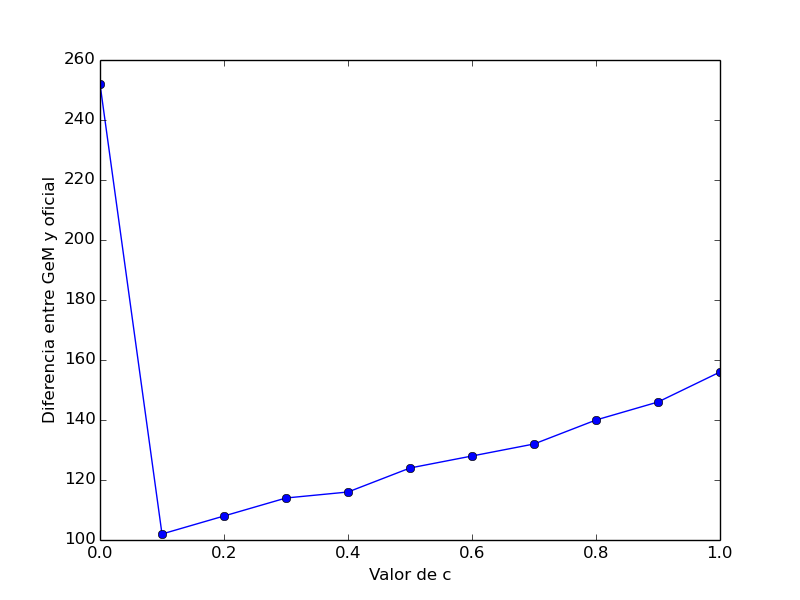
\includegraphics[width=.5\textwidth]{exp6_arg.png}}
            }
            \caption{GeM vs Primera Divisi\'on F\'utbol Argentino para $\alpha=1$}
            \label{fig:exp6_arg_1}
        \end{figure}

        \par La posición de San Martín de San Juan (13º según el puntaje
        oficial) en el ranking GeM se debe, en parte, a que le ganó a San
        Lorenzo en la fecha 3, mientras que Aldosivi (24º según el puntaje
        oficial) logró lo mismo en la fecha 10 y le gano a San Martín de San
        Juan en la fecha 22. Removiendo esos partidos sus posiciones en GeM
        bajan significativamente.

        \par De todos modos podemos observar que, para el valor de $\alpha=0.1$,
        el ranking devuelto por GeM se parece un poco más al oficial, d\'andonos
        los 6 primeros puestos que se pueden observar en el cuadro
        \ref{subfig:exp6_arg_prim}.

        \begin{figure}[H]
            \centering
            \subfloat[][Primeros Puestos\label{subfig:exp6_arg_prim}]{
                \footnotesize
                \setlength{\tabcolsep}{3pt}
                \begin{tabular}{|l|r||l|r|}
                    \hline
                    \multicolumn{2}{|c||}{GeM}&\multicolumn{2}{c|}{Oficial: 3-1-0}\\
                    \hline
                    Equipo & Puntaje & Equipo & Puntaje\\
                    \hline\hline
                    River Plate &0.0383429& San Lorenzo &50 \\
                    Boca Juniors& 0.038337& Boca Juniors &49 \\
                    San Lorenzo &0.0372973& Racing Club &46 \\
                    Racing Club &0.0363868& Rosario Central &45 \\
                    San Martín (SJ) &0.0352285& River Plate &44 \\
                    Rosario Central &0.0347587& Independiente &38\\
                    \hline
                \end{tabular}
            }\hspace{2pt}
            \subfloat[][\'Ultimos Puestos\label{subfig:exp6_arg_ult}]{
                \footnotesize
                \setlength{\tabcolsep}{3pt}
                \begin{tabular}{|l|r||l|r|}
                    \hline
                    \multicolumn{2}{|c||}{GeM}&\multicolumn{2}{c|}{Oficial: 3-1-0}\\
                    \hline
                    Equipo & Puntaje & Equipo & Puntaje\\
                    \hline\hline
                    Olimpo &0.0316438&Godoy Cruz &22\\
                    Huracán &0.0315532&Huracán &21\\
                    Godoy Cruz &0.0315278&Atlético de Rafaela &20\\
                    Atlético de Rafaela &0.0309498&Arsenal &17\\
                    Colón &0.0308694&Nueva Chicago &14\\
                    Nueva Chicago &0.0307189&Crucero del Norte &14\\
                    \hline
                \end{tabular}
            }
            \caption{GeM vs Primera Divisi\'on F\'utbol Argentino para $\alpha=0.1$}
            \label{fig:exp6_arg_2}
        \end{figure}
        \medskip

        \par De estos 6 primeros puestos de GeM, 5 efectivamente corresponden a
        esos primeros 6 lugares según el oficial (el que falta es Independiente,
        que GeM ubica 15º) y uno de ellos está en la misma posición en ambos
        rankings.

        \par Otra coincidencia notable son los últimos puestos, los cuales se
        pueden observar en el cuadro \ref{subfig:exp6_arg_ult}. Esta tabla tiene
        3 coincidencias débiles (mismos equipos en distinta posición) y una
        coincidencia exacta.\\

%%*************************************************************************
    \item En este caso, la diferencia para valores no nulos de $\alpha$ 
        es escasa, y la diferencia con el oficial en general es mucho mejor que
        para el caso del campeonato argentino. Consideramos esto relacionado al
        hecho de que hay pocos partidos en total, y a que la organización del
        torneo también se basa fuertemente en la transitividad de victorias (al
        menos en la fase final): en un Mundial, si A le ganó a B y B a C, se asume que A es
        mejor que C.

        \par Para todos los valores no nulos de $\alpha$ GeM ubicó
        correctamente como ganador a Alemania. Para $\alpha=0.1$ considero que
        el subcampeón fue Países Bajos, lo cual sorprende dado que Argentina le
        ganó ''4 a 2'' (el resultado de los penales). Evidentemente un valor tan
        bajo de $\alpha$ le da baja importancia a esto y pondera más las
        diferencias de goles de Países Bajos contra sus rivales (4 vs España, 2
        vs Chile), mucho mejores que las de Argentina (que ganó todos sus
        otros partidos por un gol de diferencia). Para todos los demás valores de
        $\alpha$, GeM identificó correctamente a Argentina como subcampeón.

        \par Las menores diferencias generales se obtuvieron para $\alpha=0.2$,
        $\alpha=0.3$ y $\alpha=0.4$ ''empatadas'' en una distancia de 50 con el
        ranking oficial de la FIFA. En estos casos sorprende la precisión de los
        resultados. Por ejemplo, observemos los primeros 8 lugares en la
        siguiente tabla, que coinciden exactamente con el ranking provisto por
        la FIFA:

        \begin{figure}[H]
            \centering
            \subfloat[][Primeros puestos $\alpha=0.4$]{
                \footnotesize
                \setlength{\tabcolsep}{3pt}
                \begin{tabular}[b]{|l|r|}
                    \hline
                    Equipo & Puntaje\\
                    \hline\hline
                    Alemania &0.0986858\\
                    Argentina &0.0764719\\
                    Países Bajos &0.0650904\\
                    Brasil &0.0480157\\
                    Colombia& 0.0419815\\
                    Bélgica &0.0405001\\
                    Francia &0.0396461\\
                    Costa Rica &0.0344357\\
                    \hline
                \end{tabular}
            }\hspace{10pt}
            \subfloat[][Diferencia en Funci\'on de $\alpha$]{
                \raisebox{-.13\height}{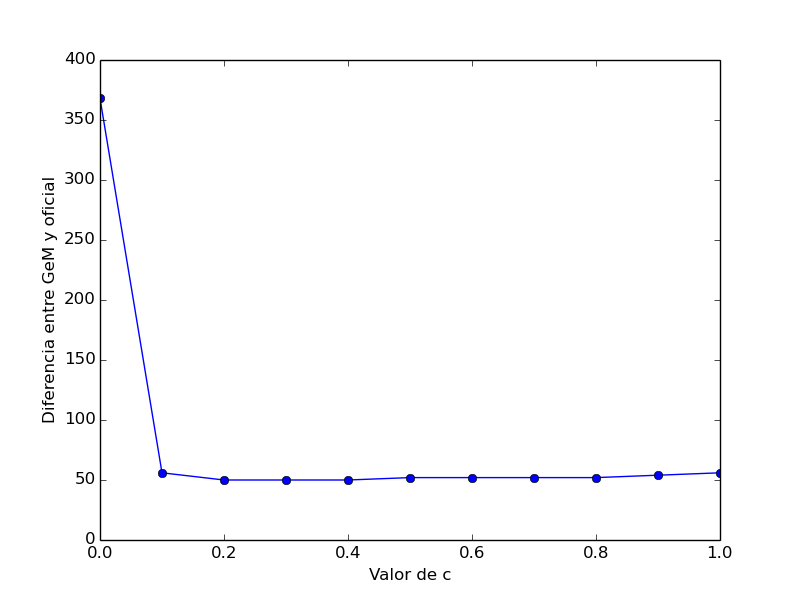
\includegraphics[width=0.5\textwidth]{exp6_2014.png}}
            }
            \caption{GeM vs Copa del Mundo 2014}
        \end{figure}

        Al consultarle su opinión al respecto de si fue o
        no penal, GeM guardó un respetuoso silencio.

%%*************************************************************************
    \item Nuevamente observamos una buena aproximación entre GeM y el ranking
        oficial. Quizás los más sorprendente es que para todos los valores no
        nulos de $\alpha$, GeM supo clasificar a Alemania Federal como el
        ganador del torneo a pesar de haber perdido por una diferencia de 5
        goles en la fase de grupos con el subcampeón Hungría. La explicación que
        le encontramos a esto se basa en que la final se disputó precisamente
        entre esos dos equipos, y Alemania Federal se consagró ganador por 3 a
        2. Esto produce que el grafo de conectividad tenga un ciclo entre esas
        dos selecciones, lo cual hace que parte del "puntaje" de Hungría vuelva
        a Alemania Federal. Todo eso sumado a la excelente campaña de este
        último en el campeonato (4 a 1 vs Turquía, 7 a 2 nuevamente vs Turquía,
        2 a 0 vs Yugoslavia y 6 a 1 vs Austria, que venía de ganar varios
        partidos también por gran diferencia) lo posiciona efectivamente como
        ganador según GeM.

        \par También para todos los valores de $\alpha$ GeM acierta en ubicar a
        Hungría como subcampeón.

        \par La menor diferencia con el ranking oficial se obtiene con
        $\alpha=0.8$ y $\alpha=0.9$. Es preciso notar que no pudimos evaluar el
        caso $\alpha=1$ por no converger para esta instancia, a diferencia de
        las dos competiciones anteriores\footnote{Sabemos por la secci\'on
        \ref{sec:introduccion} que la convergencia está asegurada solo para $0\leq\alpha <1$, pero de todos modos venimos
        ``ensayando'' con $\alpha=1$ sabiendo que dicho valor no tiene por qué hacer
        converger al m\'etodo de la potencia para nuestro $M$}.

        \par En estos dos casos, GeM acertó en los 5 primeros puestos de la
        competición, siendo estos:

        \begin{figure}[H]
            \centering
            \subfloat[][Primeros Puestos $\alpha=0.4$]{
                \footnotesize
                \setlength{\tabcolsep}{3pt}
                \begin{tabular}{|l|r|}
                    \hline
                    Equipo & Puntaje\\
                    \hline\hline
                    Alemania Federal &0.421402\\
                    Hungría &0.409884\\
                    Austria &0.0299615\\
                    Uruguay &0.0252637\\
                    Suiza &0.0169375\\
                    \hline
                \end{tabular}
            }\hspace{10pt}
            \subfloat[][Diferencia en Funci\'on de $\alpha$]{
                \raisebox{-.5\height}{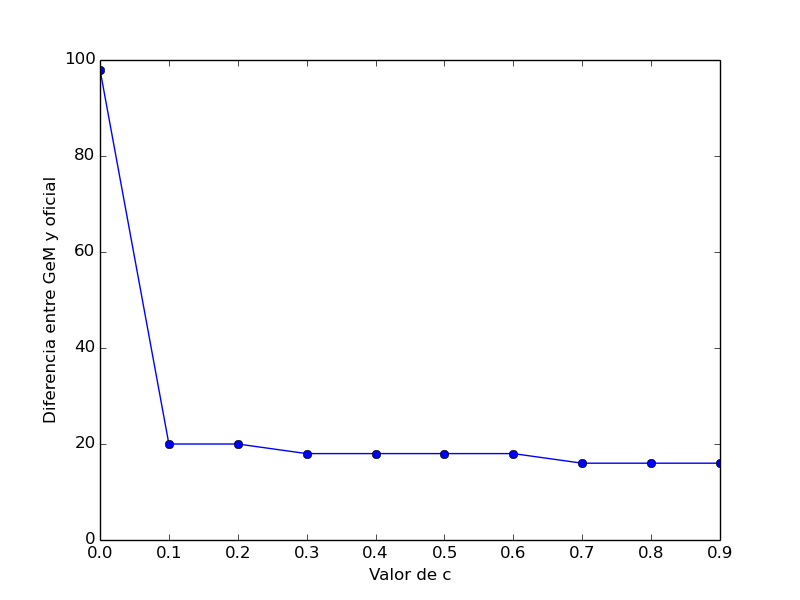
\includegraphics[width=0.5\textwidth]{exp6_1954.png}}
            }
            \caption{GeM vs Copa del Mundo 1954}
        \end{figure}
\end{enumerate}
\medskip

%%*************************************************************************
\par Lo m\'as jugoso de toda esta experimentaci\'on radica en que comparamos el
modelo GeM de rankings contra todos rankings oficiales que est\'an vigentes. El
primer resultado interesante es observar que GeM est\'a mucho m\'as cerca para
del ranking utilizado en las copas del mundo que del torneo actual del f\'utbol
argentino, y esto se ve para cualquier $\alpha\neq 0$ (el caso con $\alpha = 0$,
como ya se comentado en experimentos previos, concibe un modelo donde todos los
equipos le pueden ganar a todos con la misma probabilidad, sin importar los
resultados previos, haciendo a este par\'ametro poco interesante para analizar
por su obvia ignorancia de la realidad\footnote{¿O acaso las chances de que
Racing le gane a Crucero del Norte son las mismas de que pierda?}). A\'un as\'i,
a pesar de esta distancia, vemos que en el caso del torneo de f\'utbol
argentino, su ranking en los extremos de la ''tabla'' (particularmente en el
extremo inferior) suele ubicar a los mismos equipos que el ranking oficial. Esto
nos indica que a pesar de tener rankings muy distintos, en t\'erminos generales
ambos rankings diferencian de forma similar a los equipos ''buenos'' y
''malos''.

\par Concluyendo, vemos que GeM puede o no parecerse a otros rankings oficiales,
pero la determinaci\'on de si es mejor o peor depender\'a de qué opinen quienes
lo utilicen. Lo que si podemos afirmar es que GeM tiende a aproximarse m\'as
a los rankings oficiales (al menos los vistos) en los extremos del mismo. Es
decir, a pesar de estar a una distancia no despreciable del ranking oficial, los
equipos se\~nalados como los m\'as fuertes o mejores por ambos rankings (o los
peores) tienen varias coincidencias. Decimos entonces que, desde el punto de
vista de clasificar a un equipo como ''de los buenos'' o ''de los malos'' de la
competencia, cualquiera de los rankings dar\'ia resultados similares, pero estos
se diferencian al entrar en el detalle de qué equipo es mejor que otro.


\newpage
\subsubsection{Estabilidad de GeM}
\label{subsec:exp7}
\begin{LaTeXdescription}
    \item[Objetivo] Observar el ranking de PageRank/GeM puede sufrir variaciones
        importantes de una fecha a la otra, al recibir un set nuevo de
        informaci\'on.\\

    \item[Hip\'otesis] GeM es m\'as inestable que la puntuaci\'on oficial del
        f\'utbol.\\

    \item[Proposici\'on] Nos interesa considerar casos extremos para evaluar la
        estabilidad del ranking que devuelve GeM. El sistema de puntaje actual
        del f\'utbol tiene la caracter\'istica de ser bastante ''estable'': en
        una \'unica fecha un equipo puede ganar a lo sumo 3 puntos, lo cual
        (salvo en los comienzos de un torneo o casos de empate m\'ultiple
        dif\'iciles de encontrar en la realidad) no lo hace avanzar m\'as de 4 o
        5 posiciones.

        \par Nos interesa analizar si esta propiedad se conserva en GeM. Para
        eso, imaginemos un torneo de f\'utbol desbalanceado, es decir, un torneo
        en que al finalizar, el primer equipo tiene mucha diferencia con el
        \'ultimo\footnote{Consideramos esto desbalanceado. Si no es este el
        caso del lector, simplemente considerar una instancia que cumpla con esa
        condici\'on.}. Si en una \'ultima fecha ''inventada'', agregada
        artificialmente, el \'ultimo le ganase al primero, el m\'etodo de
        puntuaci\'on est\'andar dif\'icilmente altere demasiado el ranking.
        Queremos observar si esto ocurre con GeM.\\

    \item[M\'etodo de Experimentaci\'on] Tomamos el Campeonato de Primera B
        Nacional 2013/14, en el cual Banfield (1º) termin\'o con 78 puntos
        mientras que Villa San Carlos (22º y \'ultimo) termin\'o con 24.
        Generamos una fecha artificial extra en la que Villa San Carlos le gana
        a Banfield. El ranking oficial no cambiar\'ia, dado que con 27
        puntos Villa San Carlos seguir\'ia \'ultimo. De confirmarse nuestra
        hip\'otesis, esperar\'iamos ver un cambio en la posición que GeM le
        asigna a Villa San Carlos. En este caso, variando la cantidad de goles,
        estudiamos cu\'anto se alterar\'ia el resultado si la victoria fuese
        m\'as abultada. El valor de $\alpha$ usado fue de 0.85.\\

    \item[Resultados, an\'alisis y discusi\'on]
\end{LaTeXdescription}

\par Se confirmó la hipótesis. Efectivamente GeM altera el ranking por una
simple victoria por 1 a 0, aunque Villa San Carlos sigue último. Esto se debe a
que el puntaje GeM de Banfield cae y el de VSC sube, alterando a los demás
equipos que ganaron o perdieron contra alguno de ellos.

\begin{figure}[H]
    \centering
    \subfloat[][Distancia GeM Adulterado vs Oficial/GeM\label{subfig:exp7_dist_ranks}]{
        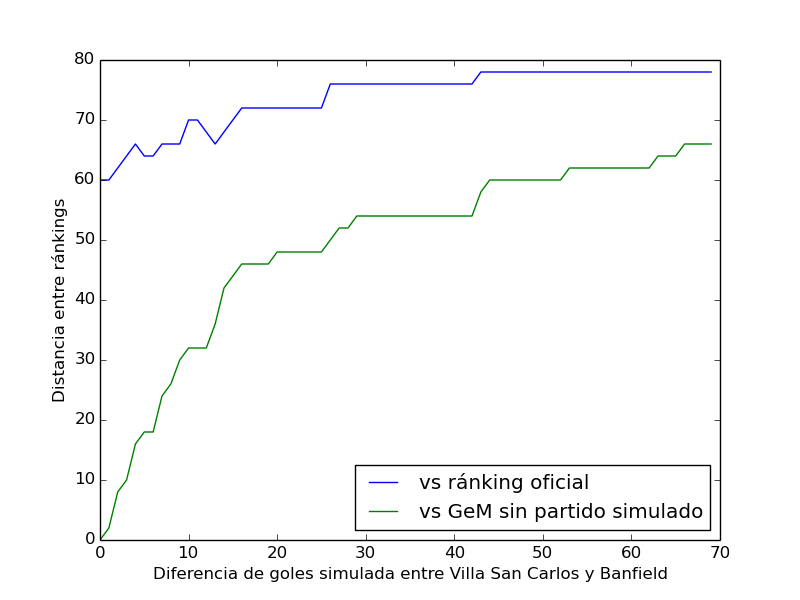
\includegraphics[width=.45\textwidth]{exp7_diferencia_ranks_funcion_goles.png}
    }\hspace{2pt}
    \subfloat[][Posición de Villa San Carlos en GeM Adulterado\label{subfig:exp7_pos_vsc}]{
        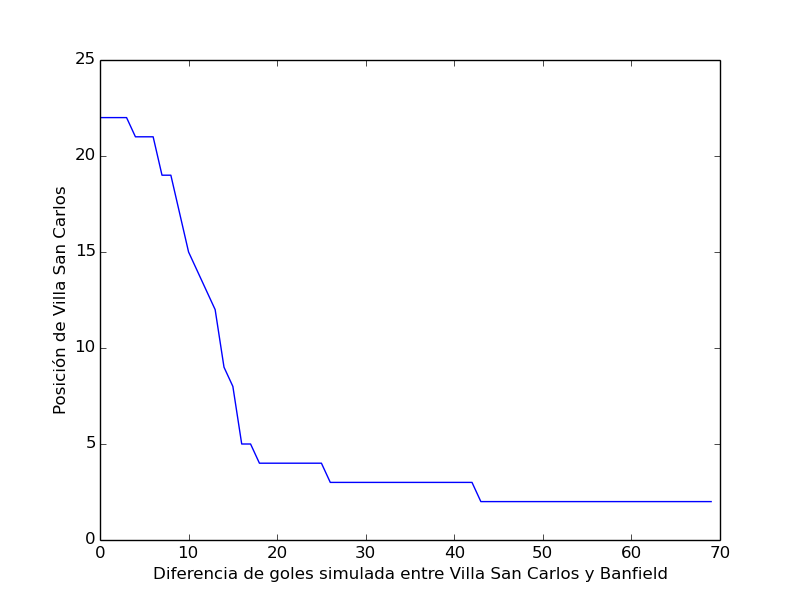
\includegraphics[width=.45\textwidth]{exp7_poscion_villa_san_carlos.png}
    }
    \caption{Consecuencias de introducir un partido artificial}
\end{figure}

\par Alcanza con una victoria de 4 a 0 para que Villa San Carlos deje el último
lugar. Y con una victoria de 43 a 0 pasa a estar en 2do lugar. Si esto parece
irreal, considerar el récord del fútbol profesional de goles en un mismo
partido: \emph{AS Adema 149 - 0 SO l'Emyrne}, el 31 de octubre de 2002 por la
\emph{THB Champions League de Madagascar}\footnote{En honor a la verdad, este
resultado fue alcanzado por goles en contra por protesta contra el arbitraje.
El resultado ``honesto'' más abultado fue \emph{Arbroath FC 36 - 0 Bon Accord
FC}, el 12 de septiembre de 1885 por la Copa Escocesa 1885-86 y, más
recientemente, el conocido \emph{Australia 31 - 0 Samoa Americana}, el 11 de
abril de 2001, por la clasificación al Mundial de Fúbol Corea-Japón 2002}.

\par En la figura \ref{subfig:exp7_pos_vsc} se puede observar la posición de
Villa San Carlos en función de la cantidad de goles del partido artificial. En
la figura \ref{subfig:exp7_dist_ranks} se puede observar la diferencia entre
rankings producida por el partido simulado en función de la cantidad de goles
del partido. Se observa claramente la ``inestabilidad'' de la que hablábamos:
por los resultados de un simple partido GeM puede alterar el orden en un factor
grande. Consideramos que esta no es una propiedad deseable del sistema, al
menos no para el fútbol: hay muchos factores que influyen en un resultado,
independientemente de la calidad de los competidores (azar, arbitraje, clima,
estado del campo, etc.). Un equipo ``malo'' no debería dejar de serlo solo por
haber haber tenido suerte (o incluso por haber hecho un único buen partido)
contra un equipo ``bueno'', o porque su rival haya hecho un partido malo.

\par El próximo experimento apunta a dejar aún más en evidencia esta situación.


\newpage
\subsection{Caso Particular GeM}
\label{subsec:exp8}
\begin{LaTeXdescription}
    \item[Objetivo] Analizar cuan ``justo'' es GeM, para un caso particular en
        el cual no haya dudas sobre lo que es justo y lo que no\footnote{O que
        haya muy poca probabilidad de que haya dudas al respecto.}.\\

    \item[Proposici\'on] Nos interesa analizar cu\'an ''justo'' es GeM para
        cierta definici\'on de justicia. Consideremos el caso de un torneo en
        que el equipo A le gana a todos los equipos salvo a B, y B pierde todos
        los partidos salvo el que le gana a A. Bajo nuestra definición de
        ''justicia'' o ''equidad'', o un aspecto de ella, A deber\'ia estar
        seguro por encima de B y B no deber\'ia estar por encima de muchos
        equipos (ya que perdi\'o contra todos). Observamos que en el caso del
        f\'utbol y su ránking 3-1-0 (o el esquema antiguo, 2-1-0) efectivamente
        B estar\'ia en la \'ultima posici\'on y A estar\'ia en la primera
        (eventualmente compartiendo dichas posiciones con alg\'un otro equipo).
        Entendemos entonces que este caso particular el ranking 3-1-0 es
        ''justo'' en este aspecto. Pero intu\'imos que esto no ser\'a lo que
        ocurra con GeM, ya que en el grafo de la instancia, A tiene un \'unico
        eje saliente (hacia B) y 18 entrantes, con lo cual su arista deber\'ia
        hacer subir mucho a B en el ranking.\\

    \item[Hip\'otesis] PageRank/GeM no es ''justo'' en cuanto al aspecto
        mencionado.\\

    \item[M\'etodo de Experimentaci\'on] Generamos una instancia de 20 equipos
        todos contra todos, donde existen A y B como se describieron. Entre los
        dem\'as equipos hacemos que el ganador sea aleatorios (con semilla =
        5). Todos los partidos terminan 1 a 0. Ejecutamos GeM y observamos el
        ranking final para diferentes valores de $\alpha$ (el factor de
        navegaci\'on).

    \item[Resultados, an\'alisis y discusi\'on] Lo primero que observamos es que B no ascendió al primer lugar para ningún valor de $\alpha$, lo cual era esperable dados los resultados del experimento 7 pero no deja de darnos cierta ``tranquilidad''. Sin embargo, y como se puede ver en la figura \ref{fig:exp8_posB}, la posición del equipo B sí mejora significativamente ya para valores pequeños de $\alpha$: ya un valor de $\alpha = 0.1$ deja a B 6to en el ránking, y a partir de $\alpha = 0.4$ pasa a estar 2do. Consideramos entonces que se confirmó nuestra hipótesis en el sentido de que GeM no es ``justo'' en un caso del estilo. Como ya postulamos en el experimento 7, no parece ``justo'' que un equipo prácticamente invicto que tuvo un ``mal día'' le permita a otro equipo salir 2do en una competencia en la que perdió con cuanto rival se cruzó.
    
    Podemos concluir entonces que los valores más ``justos'' de $\alpha$ serían los más bajos, dado que le dan menos importancia a estas situaciones extrañas pero perfectamente posibles en cualquier deporte.
    
\end{LaTeXdescription}

\begin{wrapfigure}{l}{0.5\textwidth}
    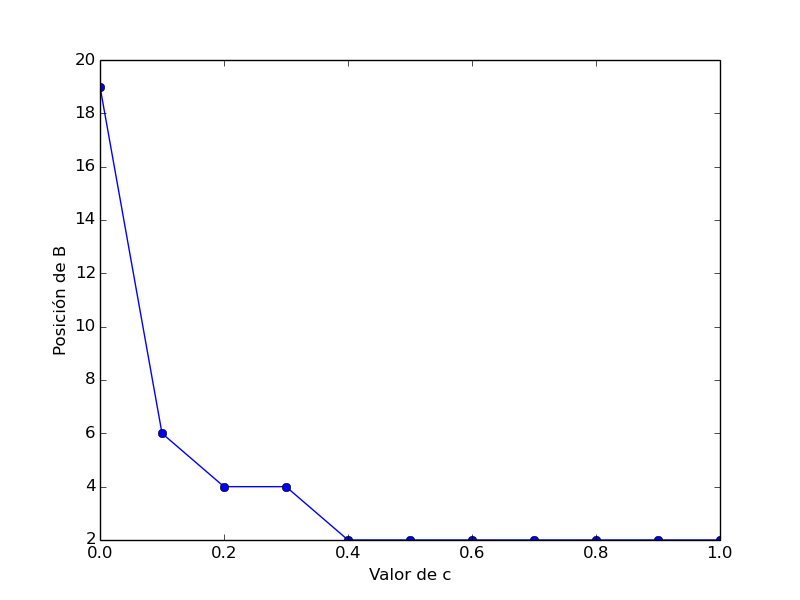
\includegraphics[width=0.5\textwidth]{exp8_posicion_B.png}
    \caption{Posici\'on del equipo B en el ranking en funci\'on del factor
        $\alpha$ ($c=\alpha$)}
    \label{fig:exp8_posB}
\end{wrapfigure}
\noindent

%---------------------------------------------------------------

\clearpage

\section{Resultados}
% TODO
% Deben incluir los resultados de los experimentos, utilizando el formato mas adecuado
% para  su  presentacion.   Deberan  especicar  claramente  a  que  experiencia  corresponde
% cada resultado.  No se incluiran aqu corridas de maquina.
\subsection{Performance}
\subsubsection{Performance de los m\'etodos en funci\'on de la discretizaci\'on para una instancia}
Utilizamos una heur\'istica para poder determinar mejor el orden c\'ubico de la curva resultado. Sea $f(x)$ el valor del tiempo de c\'omputo, graficar $f(x)/x^k$, siendo $k \in \left[ 2, 3, 4 \right] $ . De ser $f(x)$ de orden c\'ubico, esperar\'iamos que para el polinomio de orden 2 el resultado sea una funci\'on creciente, para el de orden 3 el resultado se asemeje a una constante y para el de orden 4, una funcion decreciente.

\begin{center}
\textbf{1 instancia por archivo de test}\\
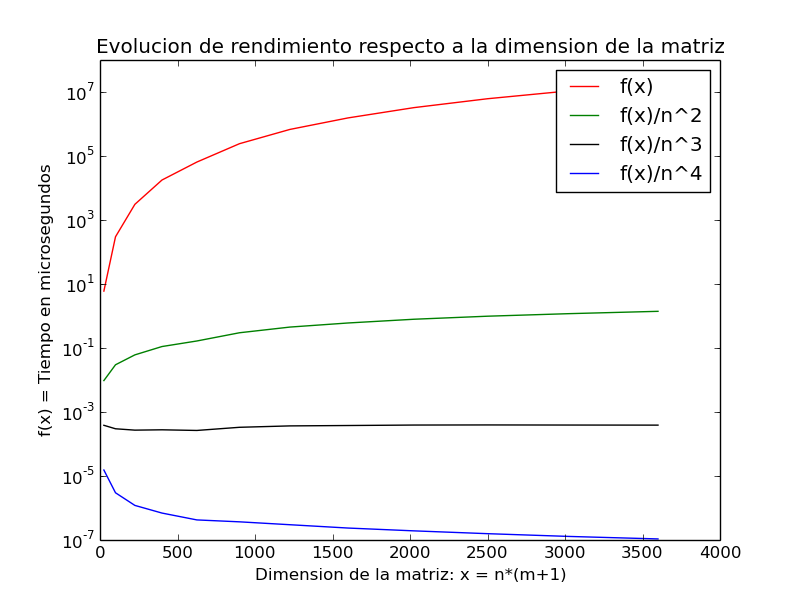
\includegraphics[scale=0.35]{experimentos2a_2b/tiempos_nm_fitteo_1_inst/eliminacion_gaussiana_time_consumed.png}
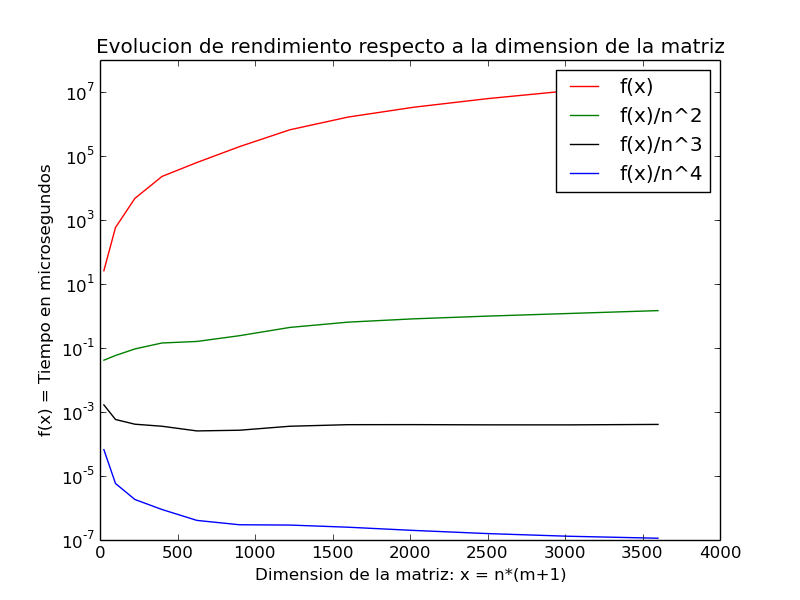
\includegraphics[scale=0.35]{experimentos2a_2b/tiempos_nm_fitteo_1_inst/factorizacion_lu_time_consumed.png}
\end{center}

A pesar de ser una heur\'istica, podemos corroborar que la curva sobre cubo se asemeja mucho a una constante, mientras que al cuadrado y a la cuarta funciones crecientes y decrecientes, respectivamente. Por lo que podemos decir que probamos emp\'iricamente que los algoritmos son del orden c\'ubico.

\subsubsection{Performance de EG vs LU variando la cantidad de instancias y la granularidad de la discretizacion}

Para comenzar esta seccion, compararemos la performance de EG vs LU variando las discretizaciones, con archivos de entrada de una sola instancia. A continuacion se presentan los graficos de comparación entre EG y LU, en diferentes escalas.

\begin{center}
\textbf{1 instancia por archivo de test}\\
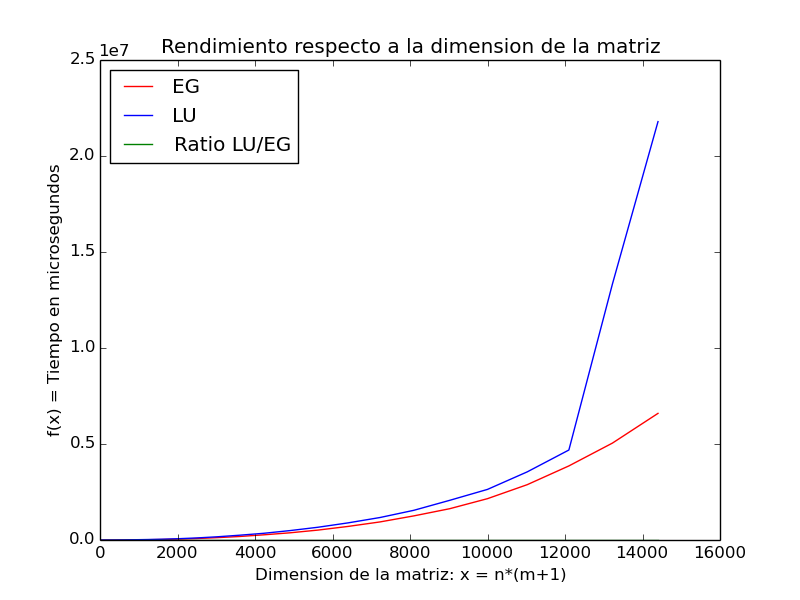
\includegraphics[scale=0.35]{experimentos2a_2b/tiempos_nm_fitteo_1_inst/gauss_vs_lu_time_consumed_abs.png}
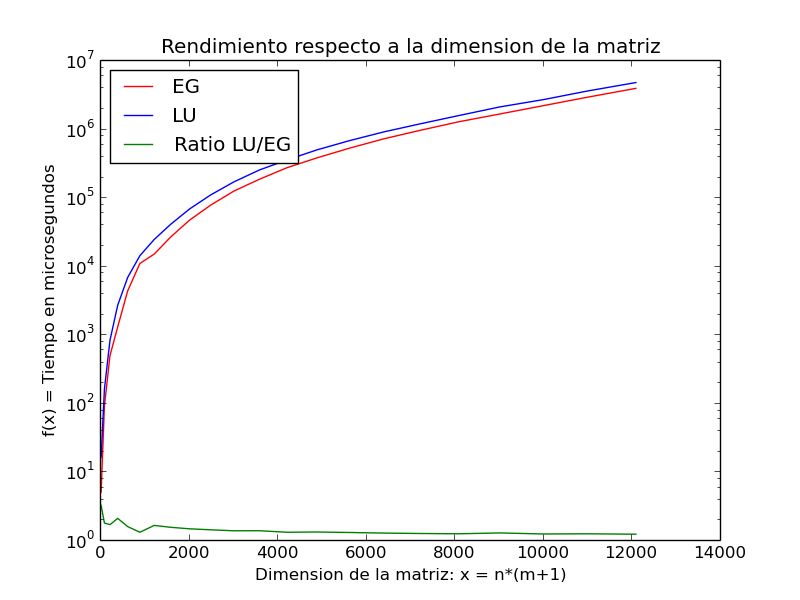
\includegraphics[scale=0.35]{experimentos2a_2b/tiempos_nm_fitteo_1_inst/gauss_vs_lu_time_consumed_log.png}
\end{center}

Dado que factorizacion LU, es identico a EG, pero guardando los coeficientes en la matriz L, tiene sentido que para una sola instancia sea mas costoso realizar la factorizacion lu y resolver el sistema que simplemente resolver usando EG.

\vspace{0.5cm}

A continuacion, se presentan graficos comparativos entre LU y EG para distintas cantidades de instancias. Lo que se observa es que, la brecha entre EG y LU se acentúa cada vez más a medida que aumenta la cantidad de instancias(ver gráficos con escala lineal). Esto se debe a que la complejidad teorica de resolver k instancias (misma matriz A, distinto vector b, en un sistema Ax=b) usando EG es $\mathcal{O}( k * (n + m)^3 )$. Por otro lado, la complejidad de resolver k instancias usando LU es $\mathcal{O}((n + m)^3 + k*(n + m)^2)$, es decir: Complejidad cúbica para hallar la descomposicion LU, y luego $k$ resoluciones de los sistemas triangulares $Ly=b$ y $Ux=y$ que cuestan orden cuadrático cada uno. 

\begin{center}
\textbf{10 instancias por archivo de test}\\
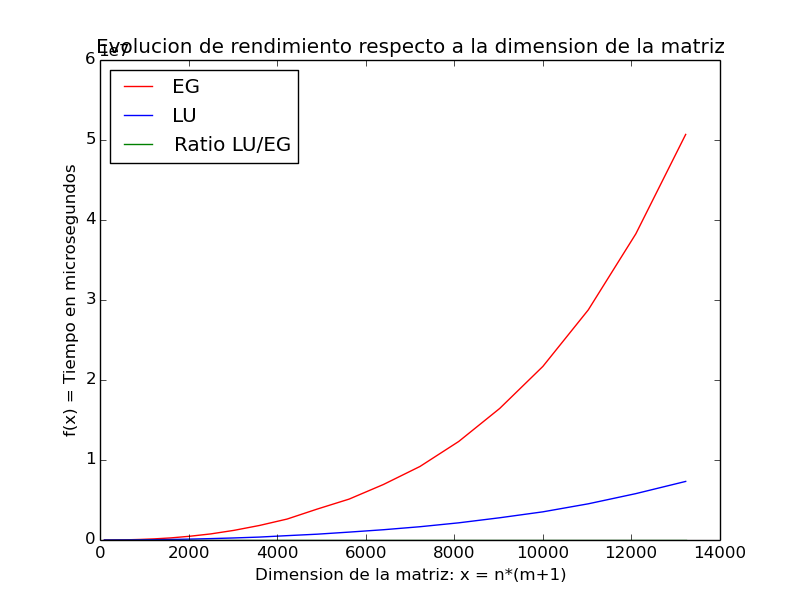
\includegraphics[scale=0.35]{experimentos2a_2b/gauss_vs_lu_10_inst/gauss_vs_lu_time_consumed_abs.png}
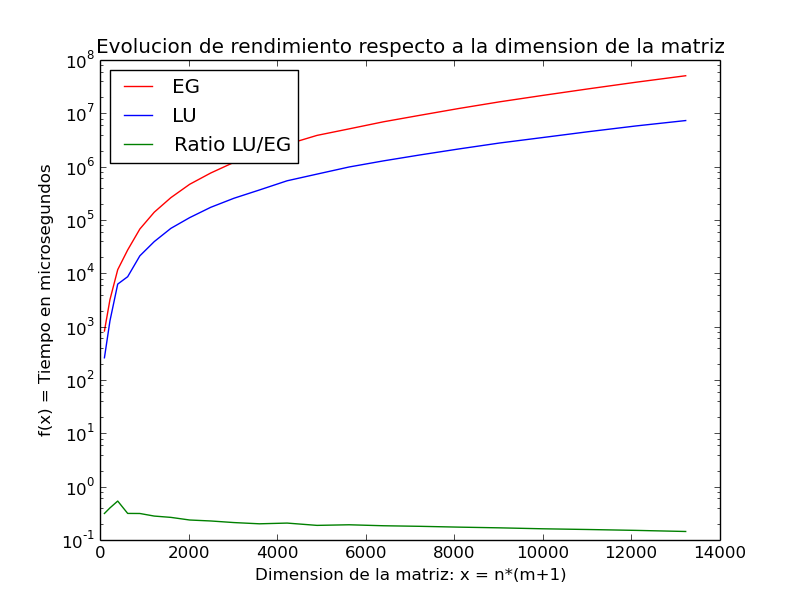
\includegraphics[scale=0.35]{experimentos2a_2b/gauss_vs_lu_10_inst/gauss_vs_lu_time_consumed_log.png}
\end{center}

\begin{center}
\textbf{50 instancias por archivo de test}\\
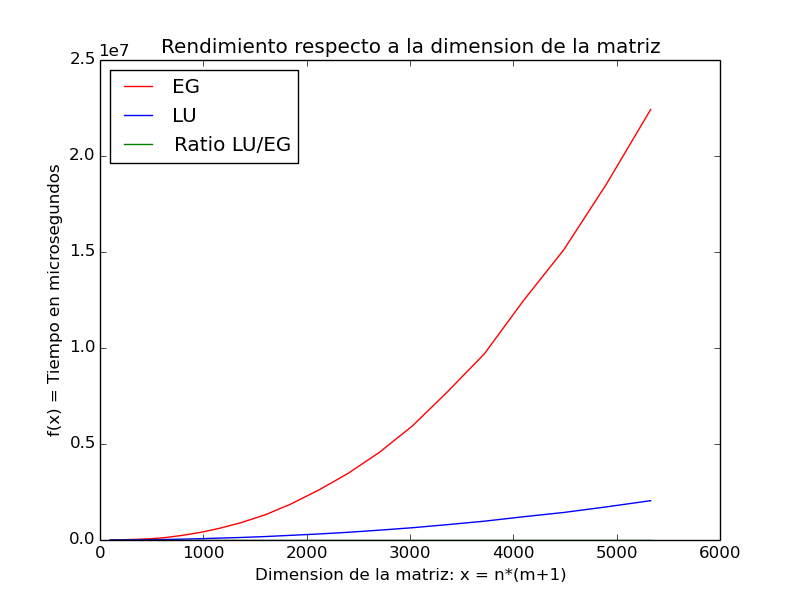
\includegraphics[scale=0.35]{experimentos2a_2b/gauss_vs_lu_50_inst/gauss_vs_lu_time_consumed_abs.png}
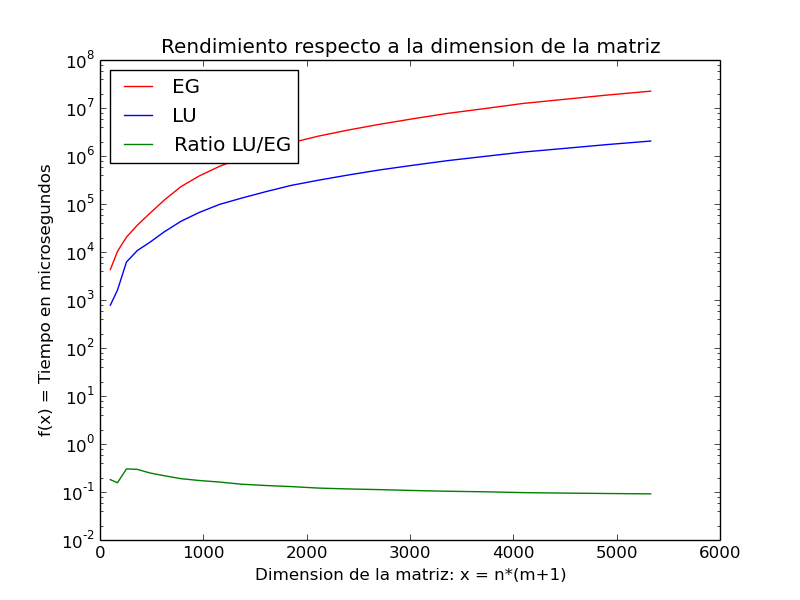
\includegraphics[scale=0.35]{experimentos2a_2b/gauss_vs_lu_50_inst/gauss_vs_lu_time_consumed_log.png}
\end{center}

\begin{center}
\textbf{150 instancias por archivo de test}\\
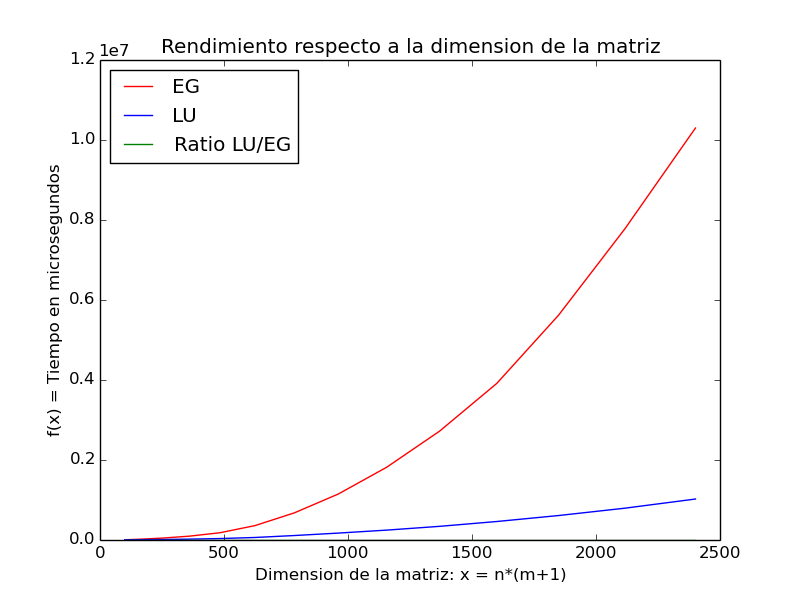
\includegraphics[scale=0.35]{experimentos2a_2b/gauss_vs_lu_150_inst/gauss_vs_lu_time_consumed_abs.png}
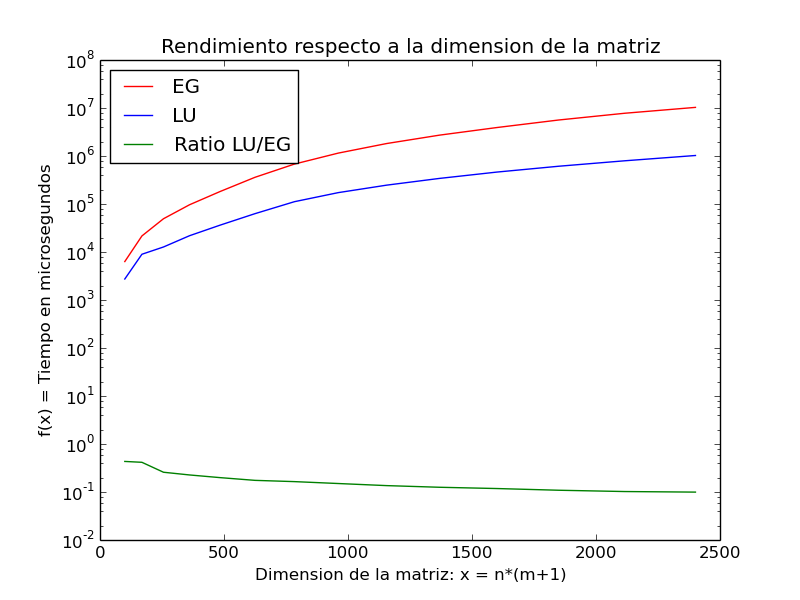
\includegraphics[scale=0.35]{experimentos2a_2b/gauss_vs_lu_150_inst/gauss_vs_lu_time_consumed_log.png}
\end{center}

\begin{center}
\textbf{500 instancias por archivo de test}\\
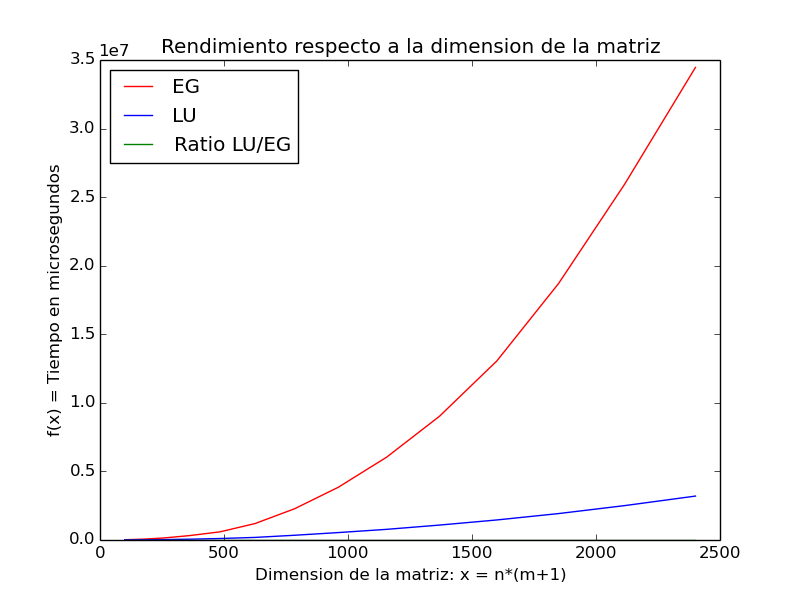
\includegraphics[scale=0.35]{experimentos2a_2b/gauss_vs_lu_500_inst/gauss_vs_lu_time_consumed_abs.png}
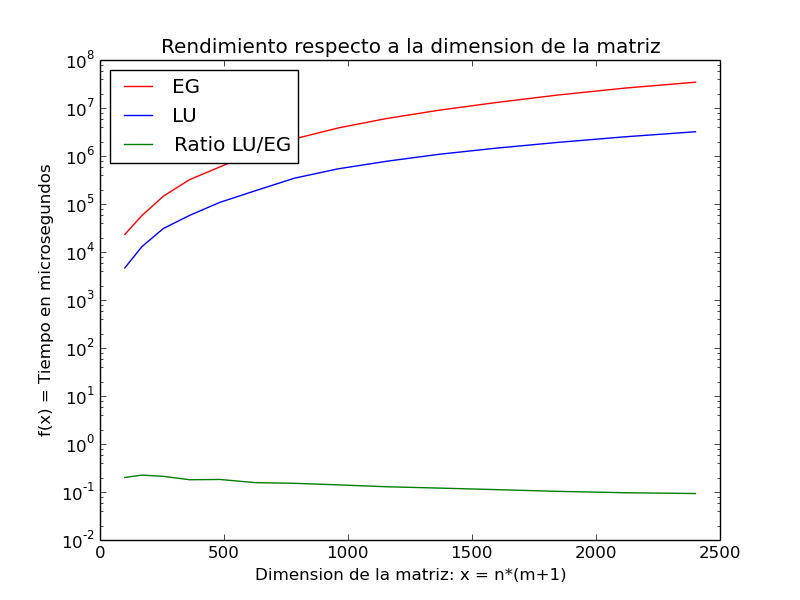
\includegraphics[scale=0.35]{experimentos2a_2b/gauss_vs_lu_500_inst/gauss_vs_lu_time_consumed_log.png}
\end{center}

Tambien se observa en los graficos con escala logaritmica que la brecha entre EG y LU para una cantidad de instancias fija se acentua a medida que se aumenta el tamaño de la matriz del sistema, pues el ratio LU/EG decrece. Creemos que esto se debe a que al dejar k fijo y aumentar $n+m$, tenemos que $\mathcal{O}((n + m)^3 + k*(n + m)^2)$ es mas pequeño que $\mathcal{O}(k*(n + m)^3)$ en terminos empíricos. 

\textbf{Consideraci\'on Adicional:} 

Luego de la experimentacion, se nos ocurrio una optimizacion de la implementaci\'on de los algoritmos, se agreg\'o la siguiente sentencia condicional al código de EG y la parte de triangulacion de LU:

\begin{lstlisting}
			.
			.
			.
for (int j = i+1; j < numfilas; j++) {

            if (abs(_A[j][i]) < EPSILON) {
                continue;
            }
			.
			.
			.
\end{lstlisting}

Es decir, si el elemento a analizar de la matriz es un cero(con tolerancia epsilon, en nuestro caso $exp(10, -9)$), el algoritmo no realiza el c\'alculo del coeficiente multiplicador ni tampoco opera sobre la fila multiplicando cada elemento por \'este. Al agregar esta sentencia y realizar los experimentos de fitteo de orden de complejidad, obtuvimos como resultado que la complejidad emp\'irica de ambos algoritmos era de orden cuadr\'atico. Creemos que esto se debe a la condición banda de la matriz, y que en muchos casos esta condición de corte evita que el algoritmo ingrese en la tercera iteracion anidada.

\subsection{Diferencia numérica de soluciones entre EG y LU}
En esta sección se mostraran los resultados de comparar las soluciones a un mismo sistema de ecuaciones $Ax=b$ usando LU y EG. Se realizo una variación en el tamaño de la matriz del sistema para ver la evolucion de las mediciones.\\

\vspace{0.3cm}

Los parámetros utilizados para el experimento fueron:
\begin{itemize}
	\item \textbf{Temperaturas internas y externas:}  externas(1500) e internas(100) \textbf{constantes} en todos los tests. 
	\item \textbf{Radio interno:} 200
	\item \textbf{Radio externo:} 400
	\item \textbf{Tamaño n de la matriz $A \in \mathbb{R}^{n \times n}$:} $[10^2\dots130^2]$
	\item \textbf{Isoterma buscada:} 500
\end{itemize}

No se mostrará ningun gráfico porque todas las mediciones de diferencia dieron cero, es decir:

\begin{itemize}
    \item $\norm{ x - \hat{x} }_\infty = 0.0 $
    \item $\norm{ x - \hat{x} }_2 = 0.0 $ 
\end{itemize}

Dado este sorprendente resultado a primera vista, hicimos un análisis mas fino del codigo y llegamos a algunas conclusiones:
\begin{itemize}
	\item El código de la resolución del problema es identico en ambos métodos desde la lectura de la entrada hasta el armado del sistema $Ax=b$, con lo cual no puede haber diferencia numérica en este tramo.
	\item El código de factorizacion lu y eliminacion gaussiana es \texttt{idéntico} salvo que LU guarda los multiplicadores en otra matriz L, tambien de precision doble, con lo cual lo único que podria acarrear LU contra EG en este tramo es el almacenamiento con error de los coeficientes.
	\item LU tambien podría acarrear error al realizar las 2 resoluciones de sistemas triangulares(contra una sola de EG)
\end{itemize}

Sin embargo, en los casos planteados esto no ocurre. Como futuro trabajo, se podrian fabricar casos de test muy especificos donde se fuercen errores numericos clásicos. (ie. sumas con números de distinto orden, restas con numeros muy cercanos, etc.) en las operaciones de resolucion de los sistemas triangulares, se esperaría que LU acarree mas error ya que realiza mas operaciones para resolver el sistema original $Ax=b$.

\subsection{Evolución estimación de la isoterma y temperatura}
Se presentarán los resultados de los experimentos en el mismo orden en que fueron planteados en la sección de desarrollo. Se realizará el análisis de los mismos en este mismo apartado.
\begin{enumerate}
	\item \begin{itemize}
				\item \textbf{Temperaturas internas y externas:} aleatorias uniformes entre $[50\dots200]$ y $[1450\dots1550]$, pero fijas entre tests.
				\item \textbf{Radio interno:} 200
				\item \textbf{Radio externo:} 400
				\item \textbf{Cantidad radios:} $[5\dots100]$
				\item \textbf{Cantidad ángulos:} 100
				\item \textbf{Isoterma buscada:} 500
			\end{itemize}
Se adjunta con el trabajo práctico un video que expone la evolución del sistema mientras se incrementa la cantidad de radios. Expondremos estáticamente algunos frames, pero es conveniente ver el video primero. Se encuentra en la misma carpeta que el pdf. (variación\_radial\_isomap.mp4, variación\_radial\_heatmap.mp4).

\vspace{0.5cm}

  	\textbf{Variación de la estimación de la isoterma entre 5 y 6 radios de discretización}\\
	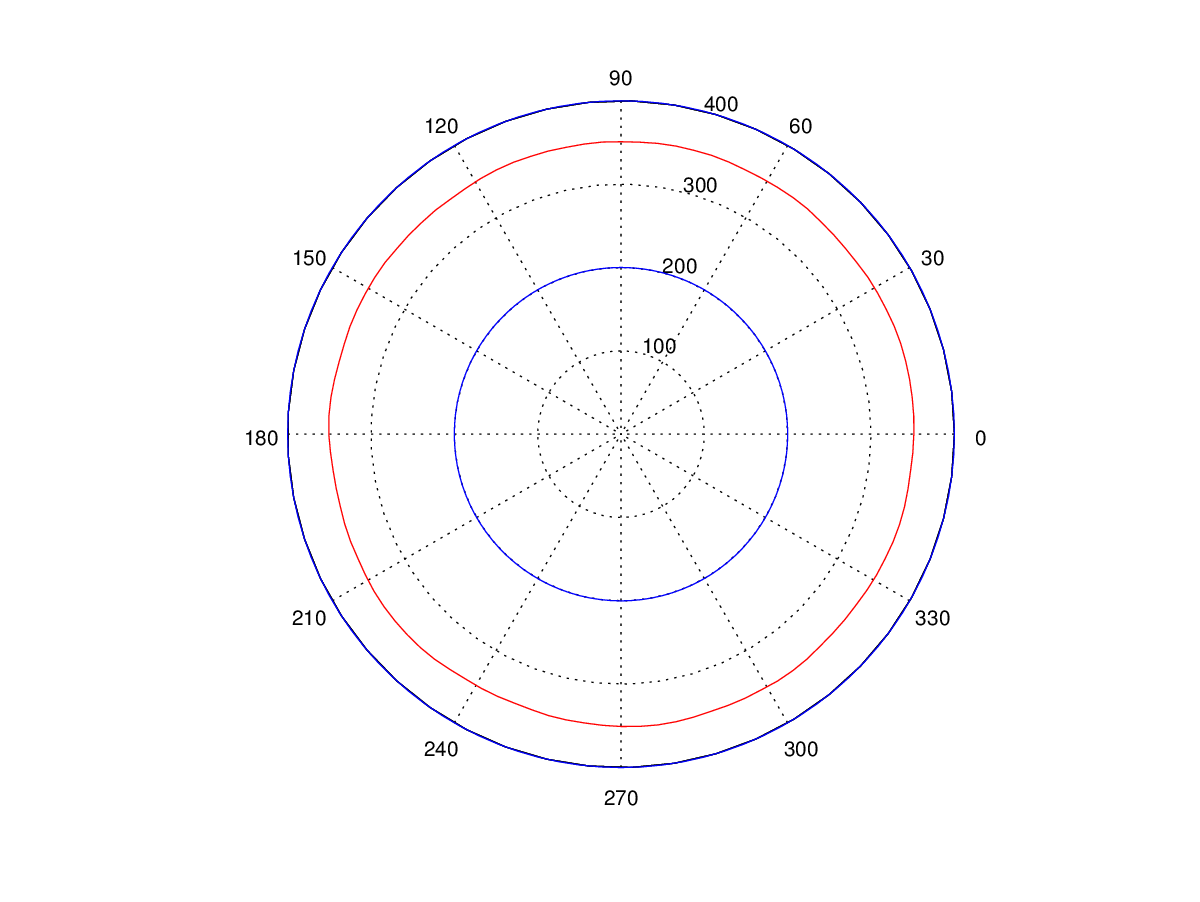
\includegraphics[scale=0.35]{experimentos1a_1b/evolucion_posicion_isoterma_temperatura/test2/test6_006_radios_inst_001_isomap.png}
	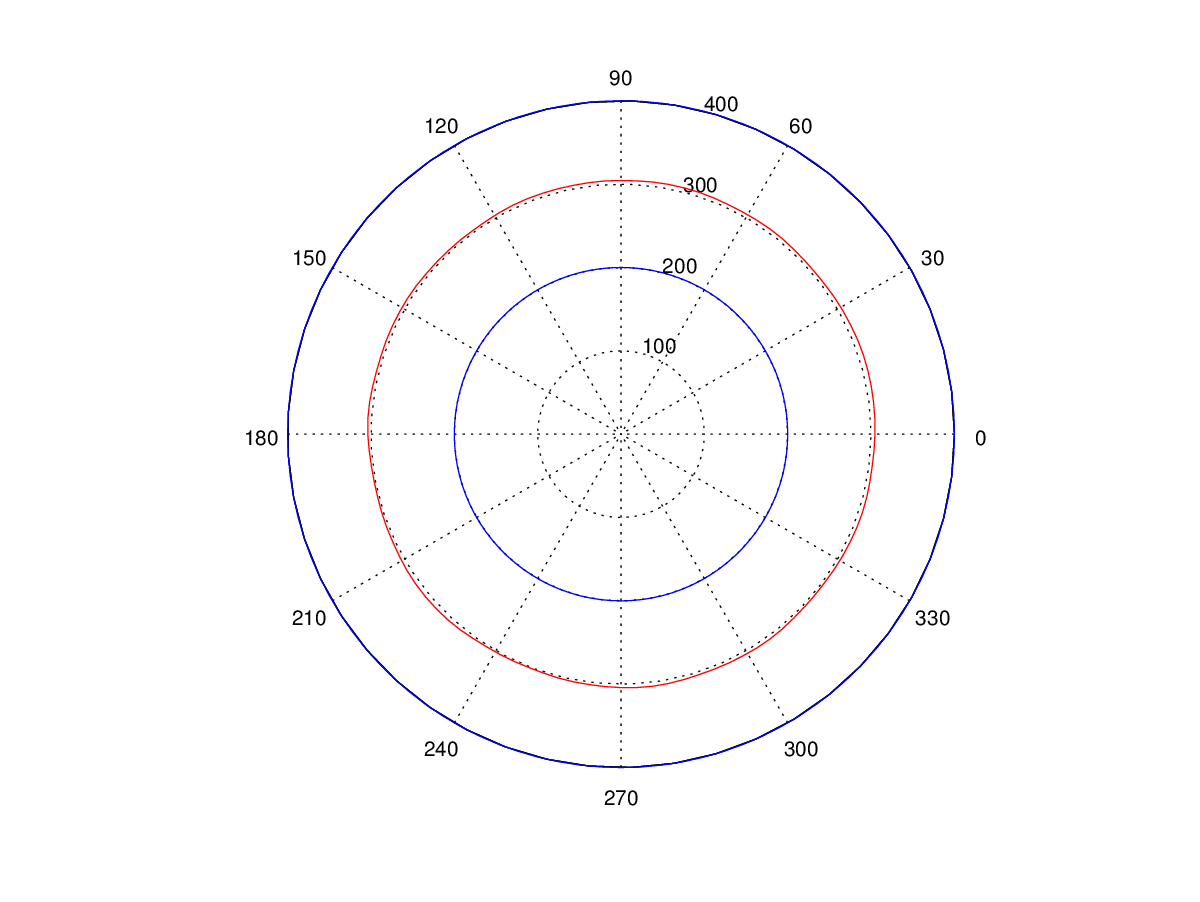
\includegraphics[scale=0.35]{experimentos1a_1b/evolucion_posicion_isoterma_temperatura/test2/test6_007_radios_inst_001_isomap.png}
	
  	\textbf{Variación de la temperatura entre 6 y 7 radios de discretización}\\
	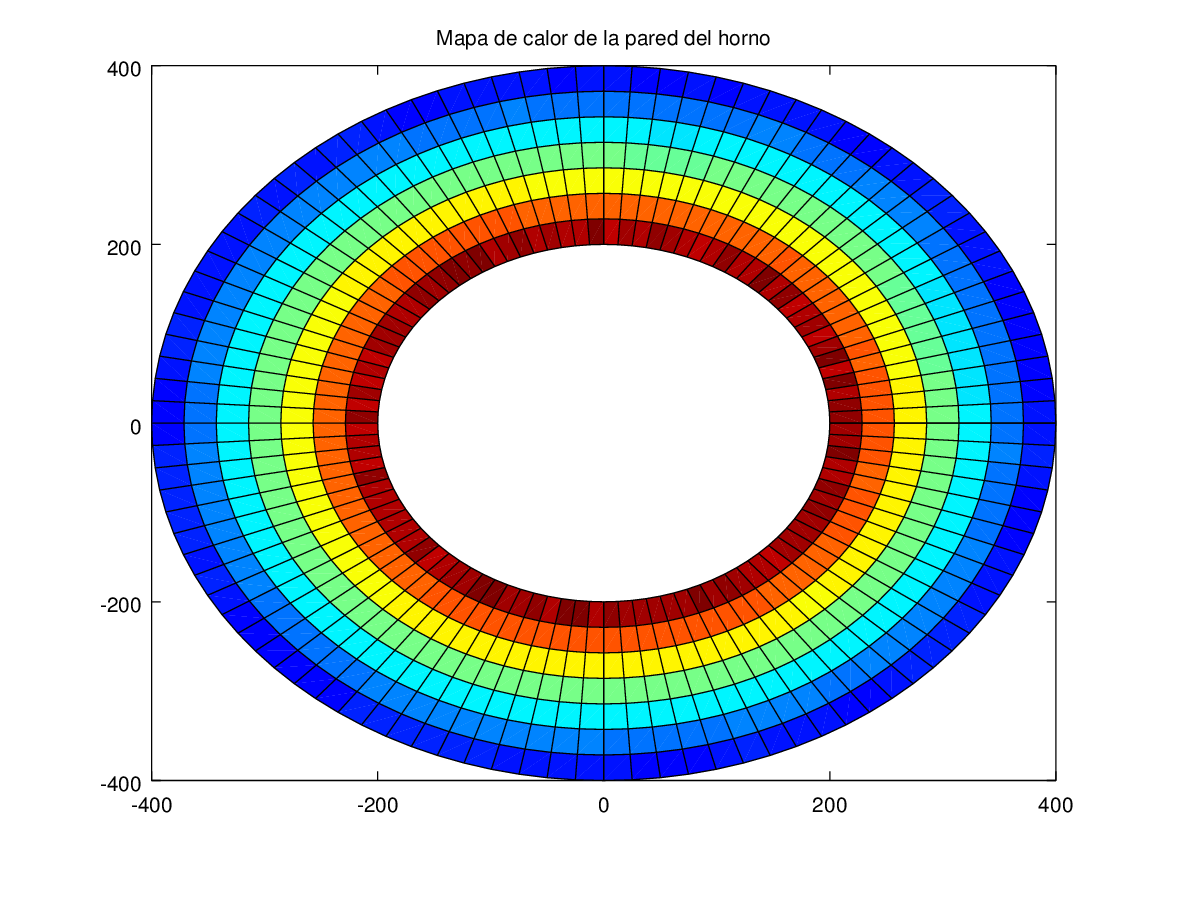
\includegraphics[scale=0.35]{experimentos1a_1b/evolucion_posicion_isoterma_temperatura/test2/test6_006_radios_inst_001_heatmap.png}
	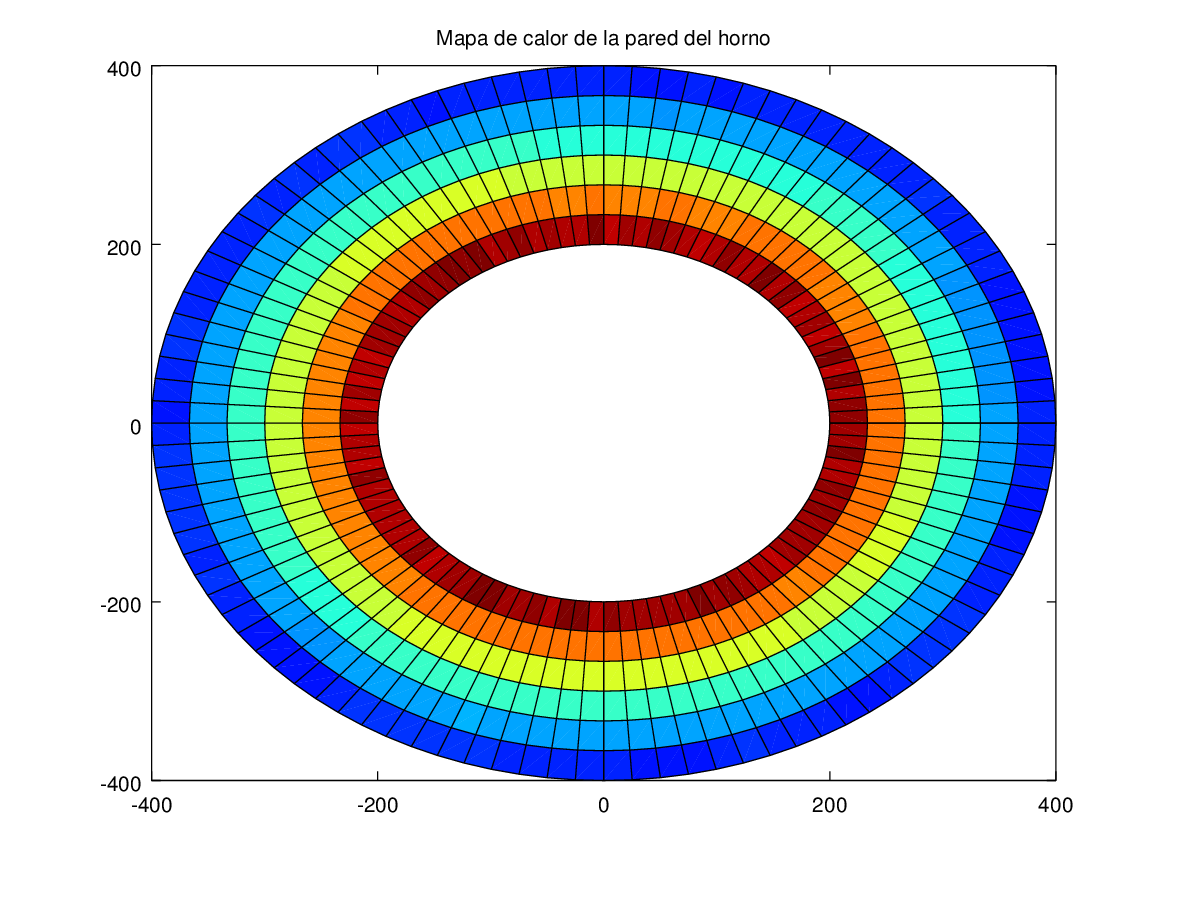
\includegraphics[scale=0.35]{experimentos1a_1b/evolucion_posicion_isoterma_temperatura/test2/test6_007_radios_inst_001_heatmap.png}

 	\textbf{Variación de la estimación de la isoterma entre 99 y 100 radios de discretización}\\
	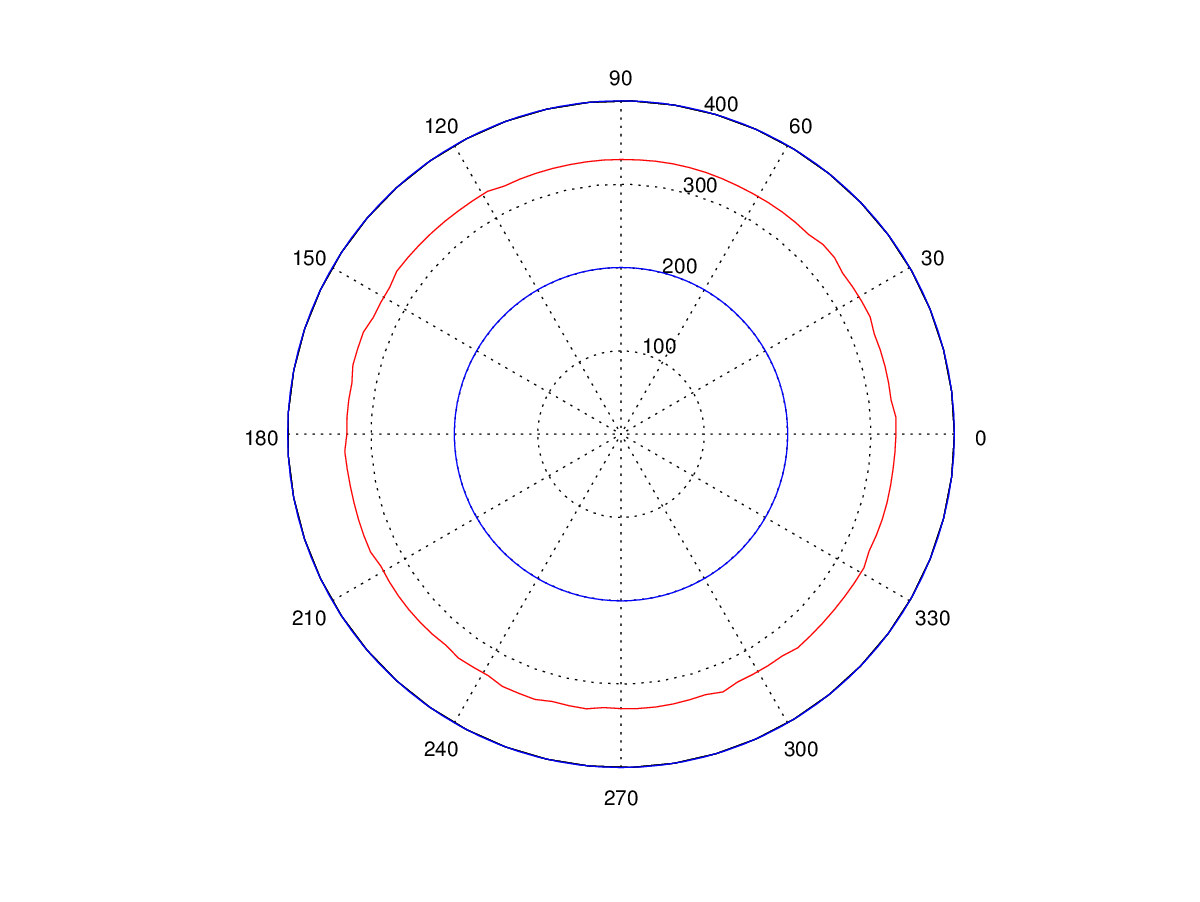
\includegraphics[scale=0.35]{experimentos1a_1b/evolucion_posicion_isoterma_temperatura/test2/test6_099_radios_inst_001_isomap.png}
	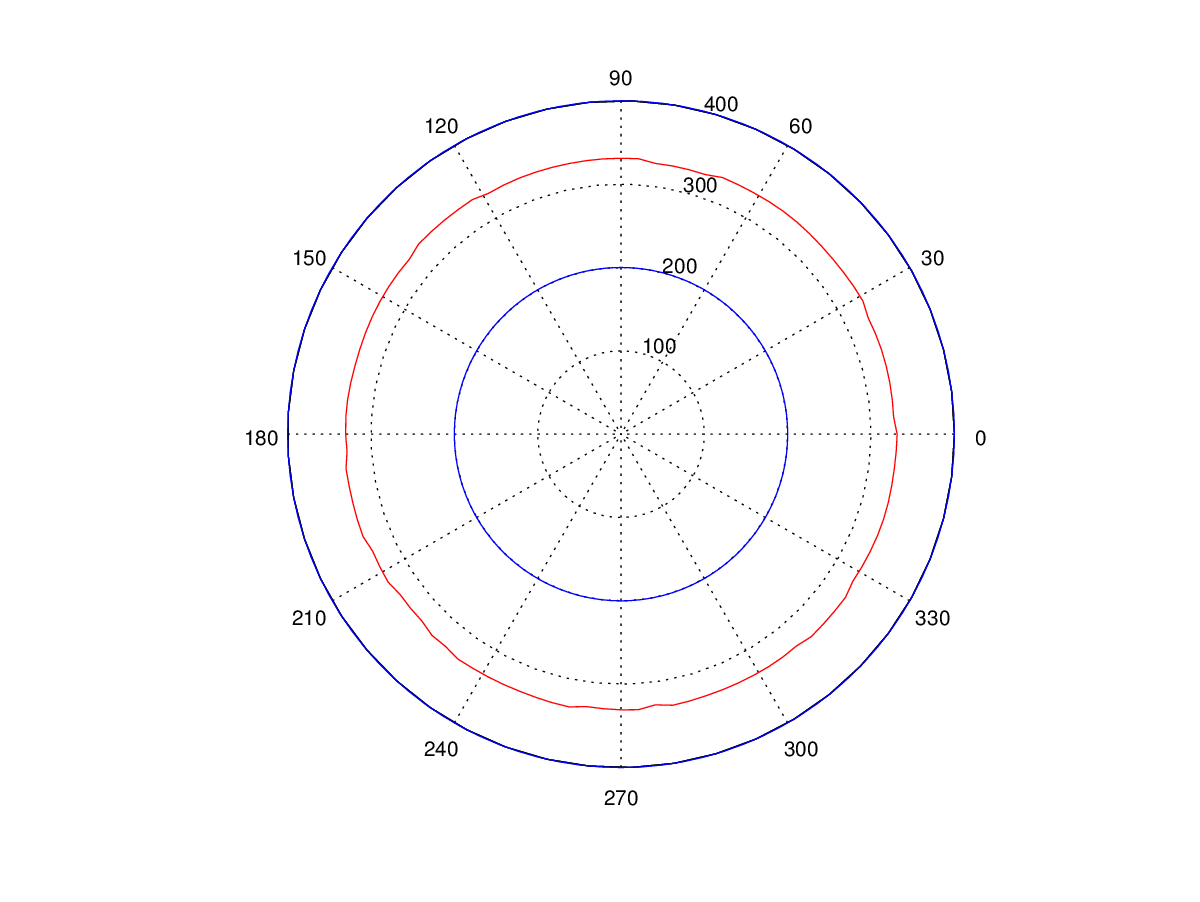
\includegraphics[scale=0.35]{experimentos1a_1b/evolucion_posicion_isoterma_temperatura/test2/test6_100_radios_inst_001_isomap.png}
	
	\textbf{Variación de la temperatura entre 99 y 100 radios de discretización}\\
	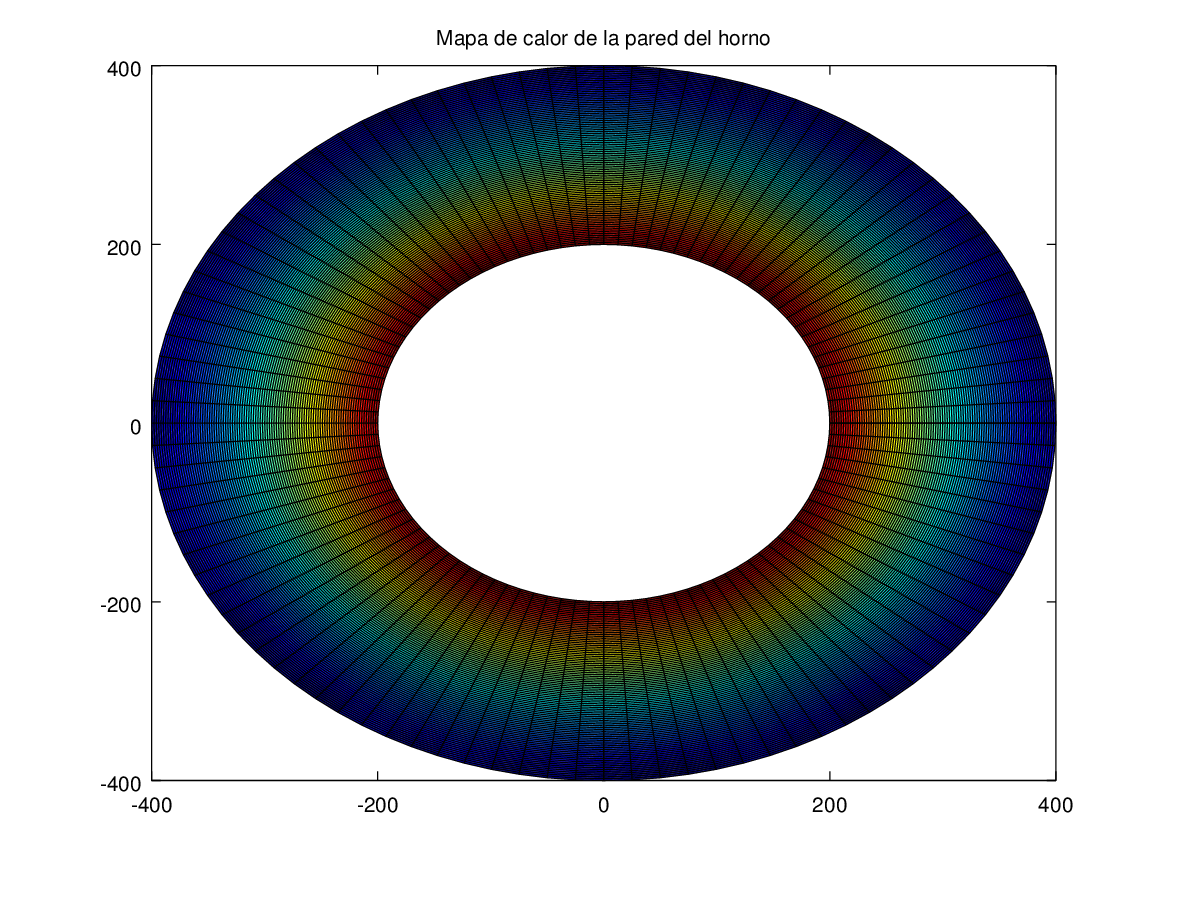
\includegraphics[scale=0.35]{experimentos1a_1b/evolucion_posicion_isoterma_temperatura/test2/test6_099_radios_inst_001_heatmap.png}
	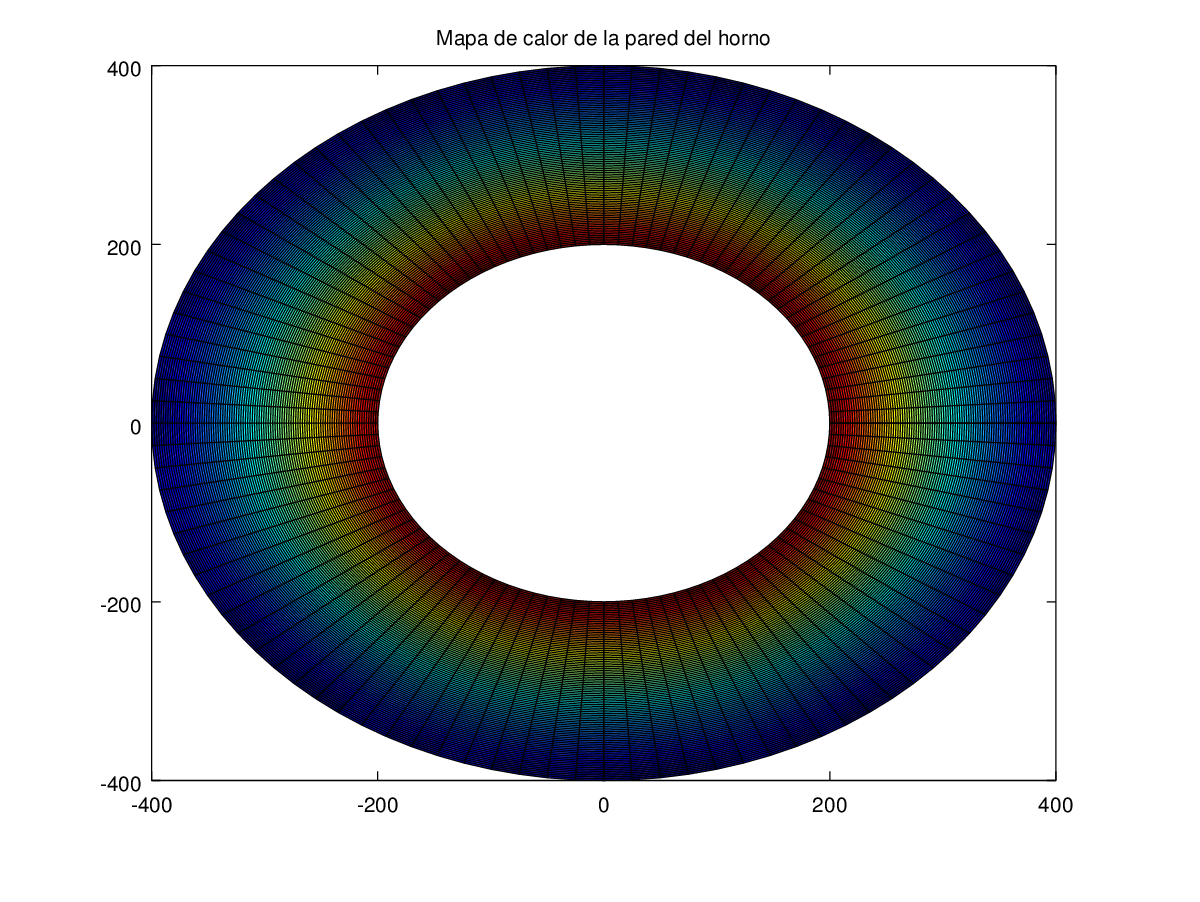
\includegraphics[scale=0.35]{experimentos1a_1b/evolucion_posicion_isoterma_temperatura/test2/test6_100_radios_inst_001_heatmap.png}

\vspace{0.5cm}

Se observa es que a medida que se aumenta la cantidad de radios de la discretización, la variación radial de la curva de la isoterma disminuye entre tests, es decir, se hace más fina la estimación, de forma tal que entre $i$ e $i+1$ radios la diferencia de la posición de la isoterma es menor a medida que $i$ crece. Para ver mejor esto se graficaron, para cada test de $i$ cantidad de radios de la discretización, el máximo y el promedio radial de la isoterma.

	\textbf{Evolución de la variación radial de la isoterma con cantidad creciente de radios}\\
	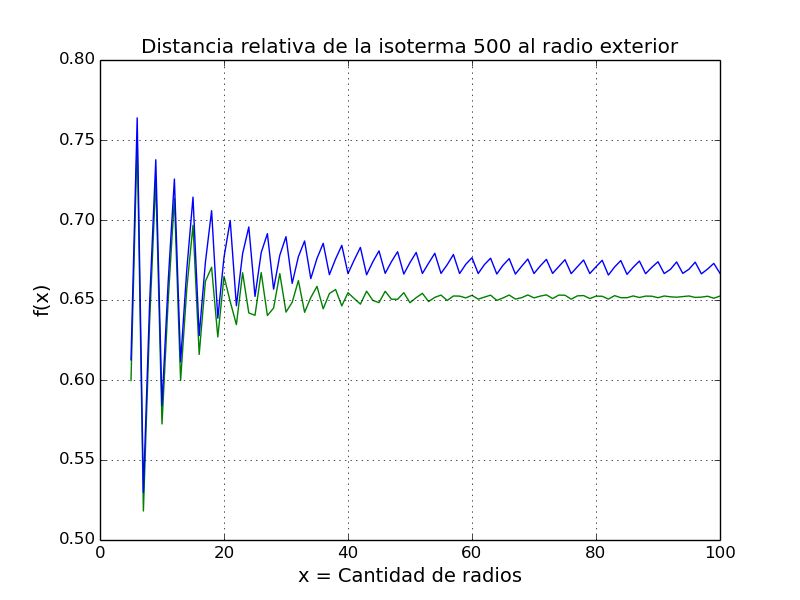
\includegraphics[scale=0.5]{experimentos1a_1b/evolucion_estimacion_seguridad_isoterma/100ang_5to100radios.png}\\


Para evitar distorsiones en el experimento anterior, se realizo otro muy similar al anterior pero con condiciones de borde \textbf{constantes e iguales}.
\begin{itemize}
	\item \textbf{Temperaturas internas y externas:} constantes, 100 y 1500. Esto es para que tenga la misma solución cada test del experimento.
	\item \textbf{Radio interno:} 200
	\item \textbf{Radio externo:} 400
	\item \textbf{Cantidad radios:} $[10\dots200]$
	\item \textbf{Cantidad ángulos:} 75
	\item \textbf{Isoterma buscada:} 500
\end{itemize}

No expondremos los resultados acerca de la evolucion de la temperatura y posicion de la isoterma, pues son similares al experimento anterior, la isoterma converge a medida que aumenta la cantidad de radios utilizada en la discretización. Al ser temperaturas constantes en este caso, la isoterma es un círculo perfecto. En el experimento anterior, la isoterma tenia pequeñas(casi imperceptibles) irregularidades dadas las condiciones aleatorias(con baja varianza) de borde.

\vspace{0.3cm}

Respecto al gráfico del promedio/maximo de la isoterma a medida que aumentan los radios, se tiene lo siguiente.

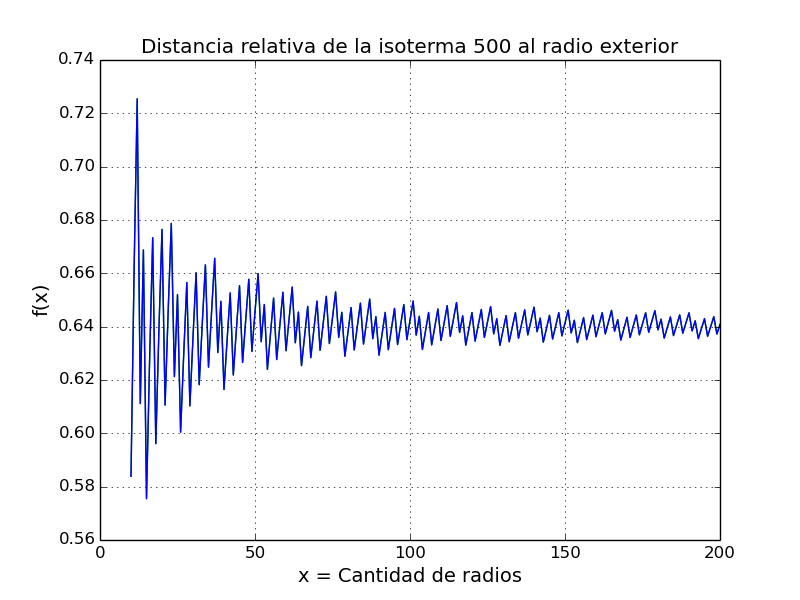
\includegraphics[scale=0.5]{experimentos1a_1b/evolucion_estimacion_seguridad_isoterma/75ang_10to200rad_evol_maxpromradio.png}\\
\textbf{Nota:} Al ser las condiciones de borde iguales, la isoterma tiene radio constante para cada experimento, con lo cual maximo y promedio coinciden, con lo cual se ve una sola curva.

\vspace{0.2cm}

Se puede ver que, al igual que en el experimento anterior, al aumentar la cantidad de radios, la posicion de la isoterma converge. Tambien se observa que en ambos experimentos, la posicion relativa de la isoterma converge aproximadamente a 0.64/0.66, lo cual tiene sentido ya que el experimento anterior tenia temperaturas aleatorias uniformes, pero \texttt{casi} alrededor de las temperaturas fijadas en el segundo experimento.\\

	\item \begin{itemize}
					\item \textbf{Temperaturas internas y externas:} constantes, 100 y 1500. Esto es para que tenga la misma solución cada test del experimento.
					\item \textbf{Radio interno:} 200
					\item \textbf{Radio externo:} 400
					\item \textbf{Cantidad radios:} 50
					\item \textbf{Cantidad ángulos:} $[5\dots50]$
					\item \textbf{Isoterma buscada:} 500
				\end{itemize}
	Se adjunta con el trabajo práctico un video que expone la evolución del sistema mientras se incrementa la cantidad de radios. Expondremos estáticamente algunos frames, pero es conveniente ver el video primero. Se encuentra en la misma carpeta que el pdf. (variación\_angular\_isomap.mp4, variación\_angular\_heatmap.mp4).

	\vspace{0.5cm}
	  	\textbf{Variación de la estimación de la isoterma entre 5 y 6 ángulos de discretización}\\
		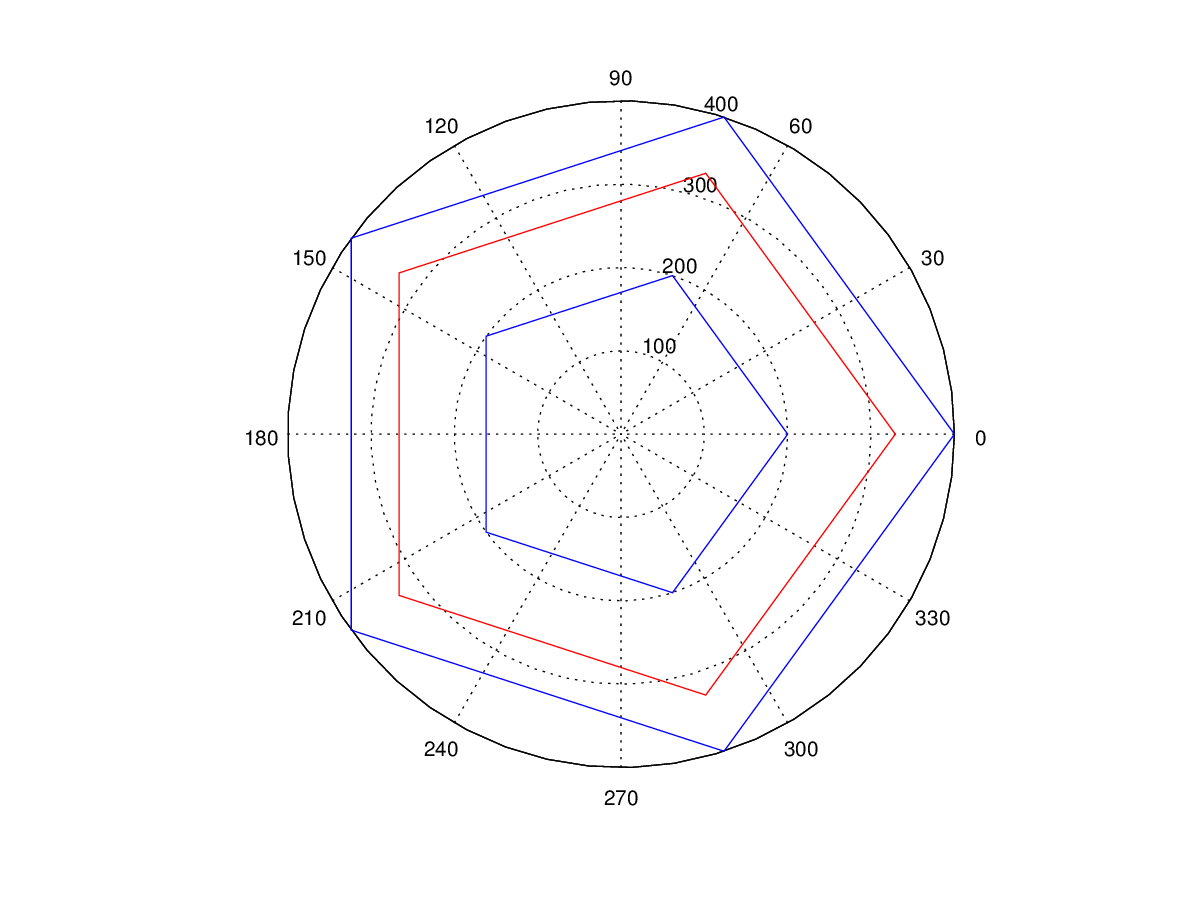
\includegraphics[scale=0.35]{experimentos1a_1b/evolucion_posicion_isoterma_temperatura/variacion_angulos_radio_fijo_se_suaviza_isoterma/test10_050_radios_005_angulos_inst_001_isomap.png}
		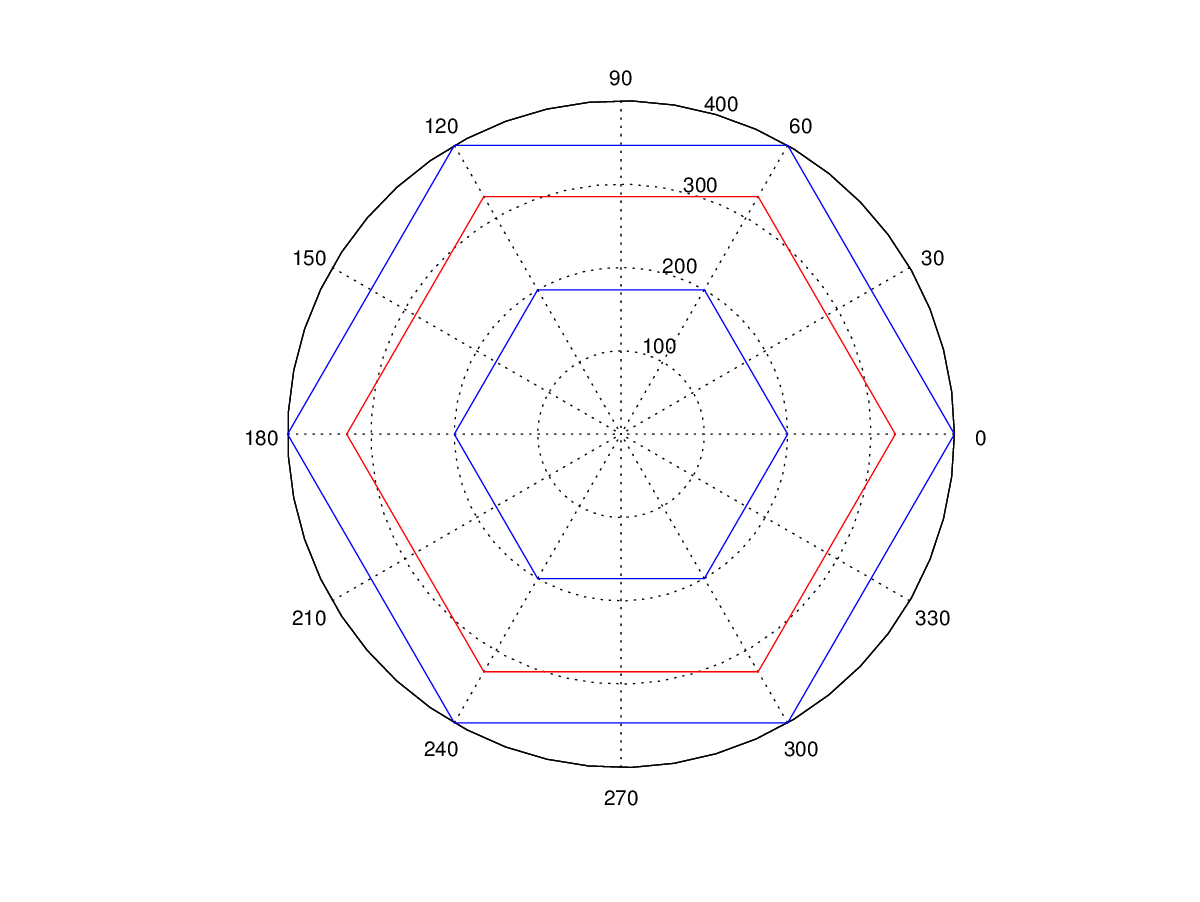
\includegraphics[scale=0.35]{experimentos1a_1b/evolucion_posicion_isoterma_temperatura/variacion_angulos_radio_fijo_se_suaviza_isoterma/test10_050_radios_006_angulos_inst_001_isomap.png}

	  	\textbf{Variación de la temperatura entre 5 y 6 ángulos de discretización}\\
	  	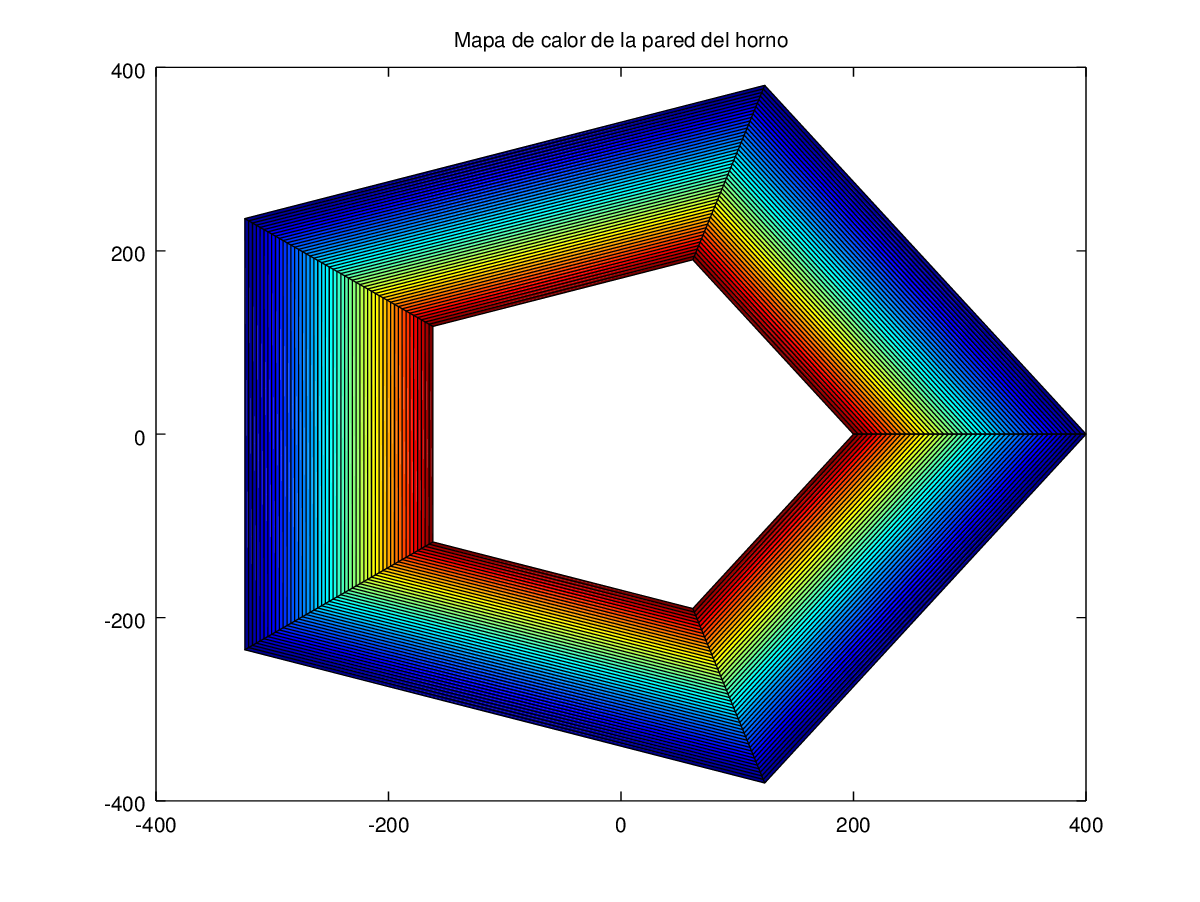
\includegraphics[scale=0.35]{experimentos1a_1b/evolucion_posicion_isoterma_temperatura/variacion_angulos_radio_fijo_se_suaviza_isoterma/test10_050_radios_005_angulos_inst_001_heatmap.png}
		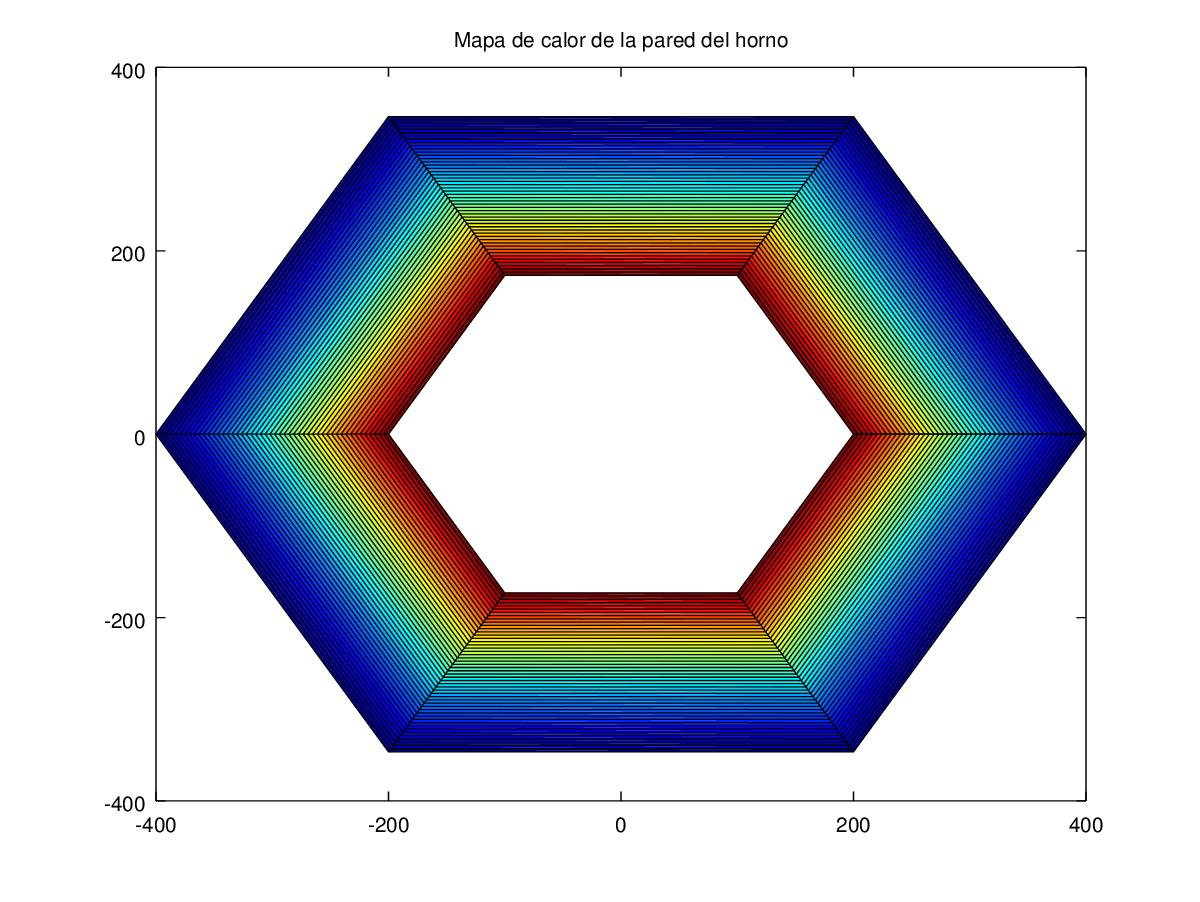
\includegraphics[scale=0.35]{experimentos1a_1b/evolucion_posicion_isoterma_temperatura/variacion_angulos_radio_fijo_se_suaviza_isoterma/test10_050_radios_006_angulos_inst_001_heatmap.png}	  	

	  	\textbf{Variación de la estimación de la isoterma entre 49 y 50 ángulos de discretización}\\
		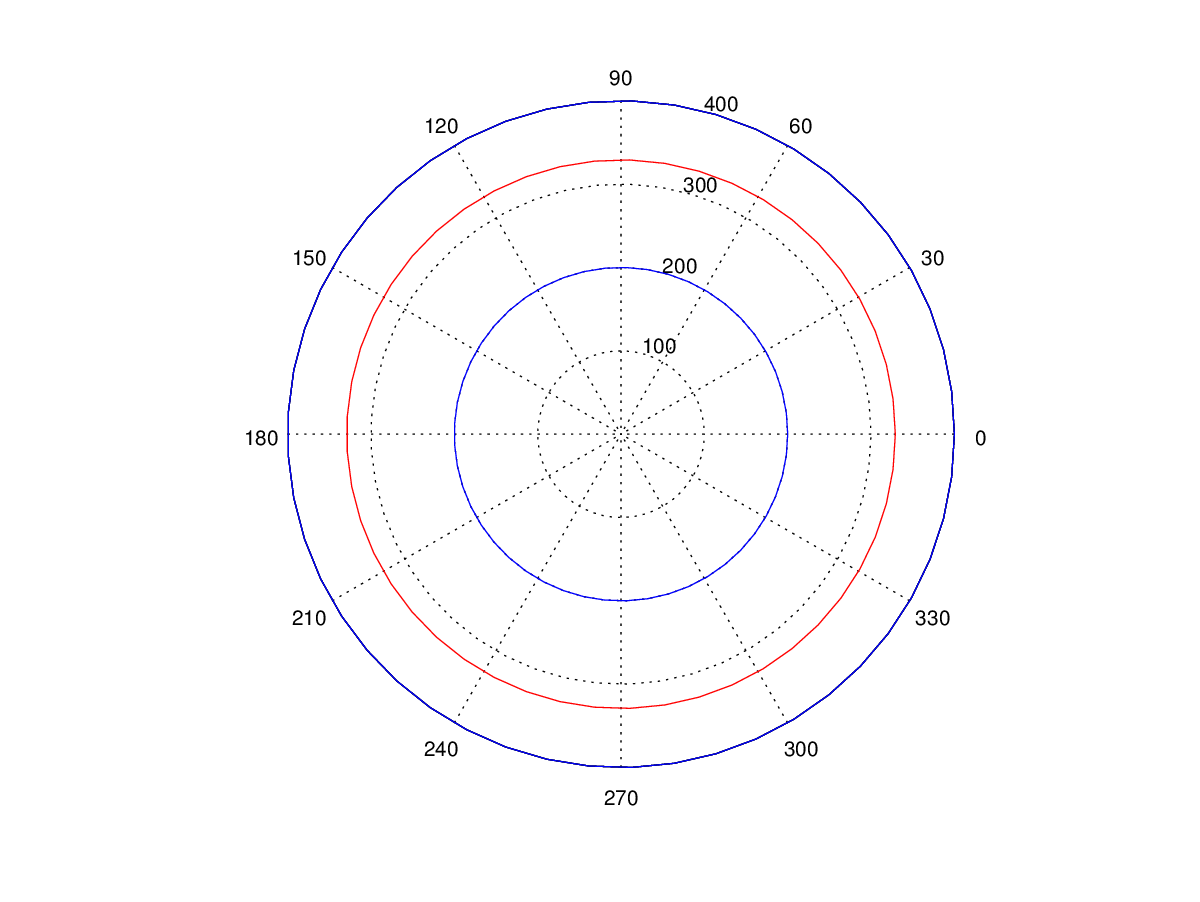
\includegraphics[scale=0.35]{experimentos1a_1b/evolucion_posicion_isoterma_temperatura/variacion_angulos_radio_fijo_se_suaviza_isoterma/test10_050_radios_049_angulos_inst_001_isomap.png}
		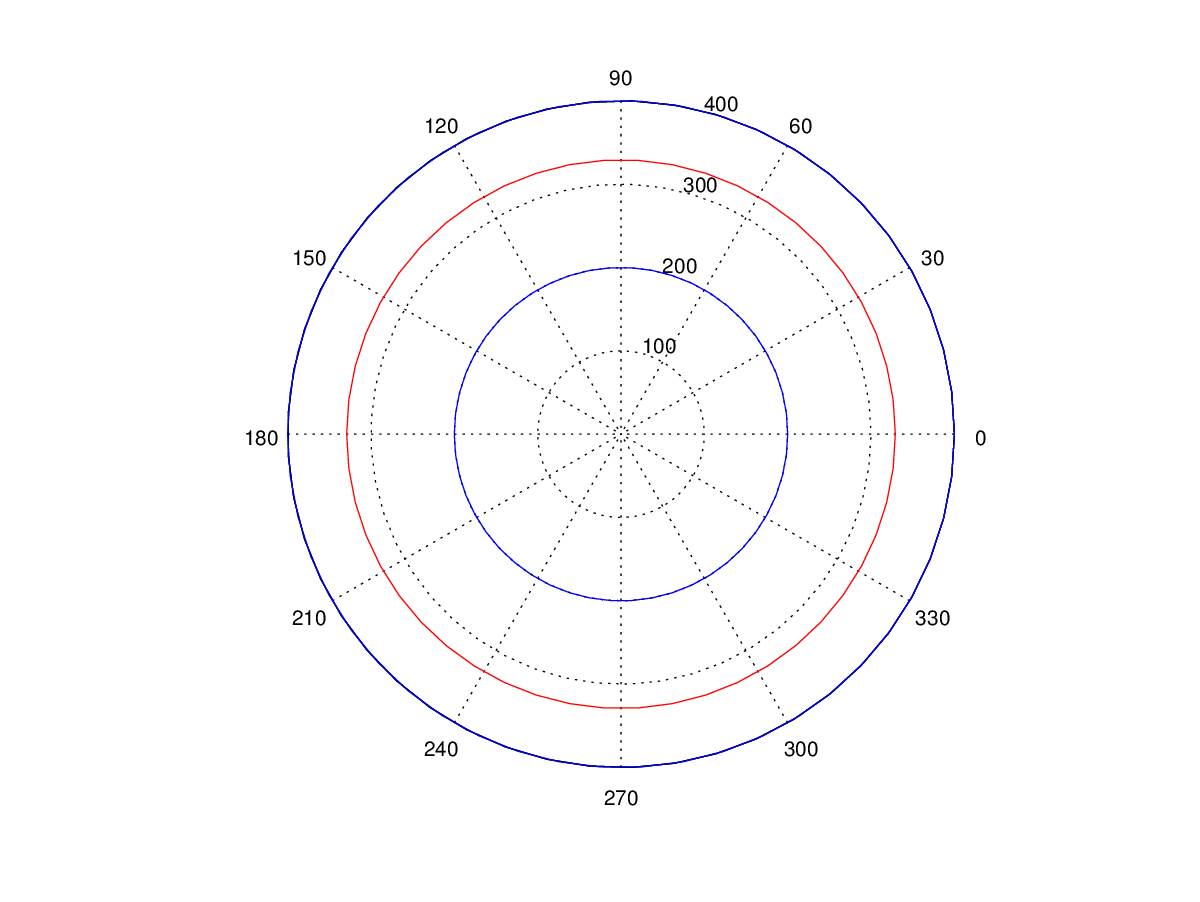
\includegraphics[scale=0.35]{experimentos1a_1b/evolucion_posicion_isoterma_temperatura/variacion_angulos_radio_fijo_se_suaviza_isoterma/test10_050_radios_050_angulos_inst_001_isomap.png}

		\textbf{Variación de la temperatura entre 49 y 50 ángulos de discretización}\\
	  	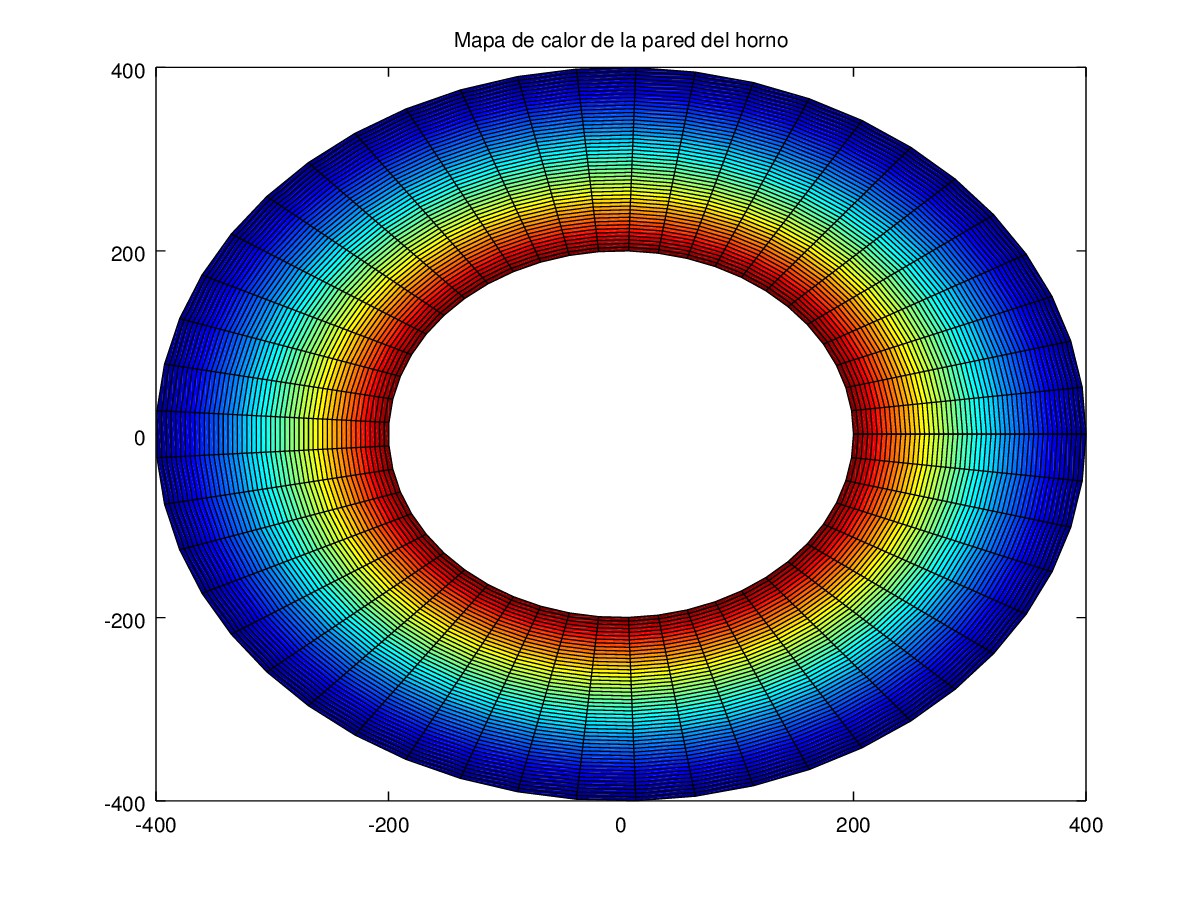
\includegraphics[scale=0.35]{experimentos1a_1b/evolucion_posicion_isoterma_temperatura/variacion_angulos_radio_fijo_se_suaviza_isoterma/test10_050_radios_049_angulos_inst_001_heatmap.png}
		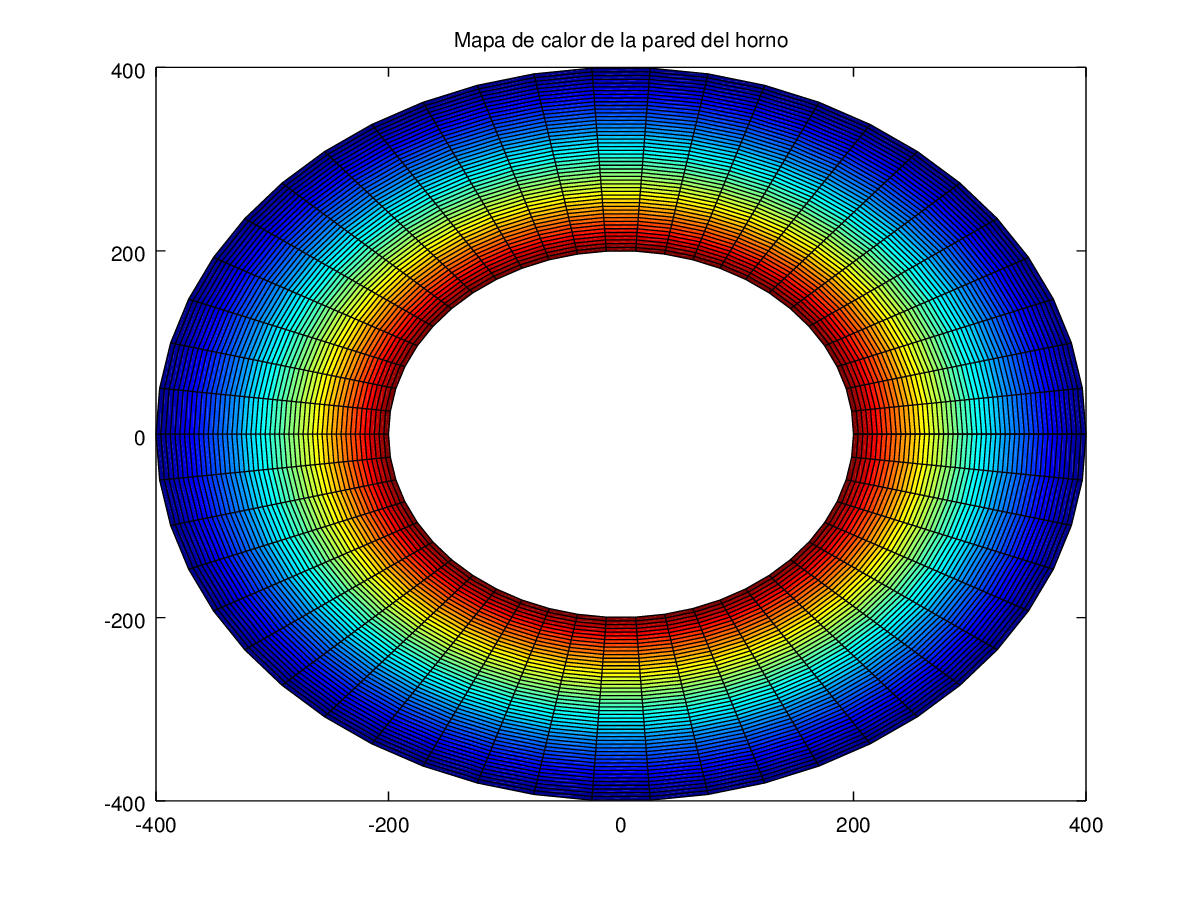
\includegraphics[scale=0.35]{experimentos1a_1b/evolucion_posicion_isoterma_temperatura/variacion_angulos_radio_fijo_se_suaviza_isoterma/test10_050_radios_050_angulos_inst_001_heatmap.png}

\vspace{0.5cm}

Aquí el radio es el mismo, pero se gana en precisión al tener más ángulos por no tener que linealizar la posición de la isoterma angularmente. Nuevamente, la posición entre dos tests consecutivos se estabiliza al aumentar la cantidad de ángulos. Tambien se observa que al cambiar el $\Delta_\theta$ los ángulos entre tests consecutivos no son los mismos.

	\item \begin{itemize}
						\item \textbf{Temperaturas internas y externas:} constantes, 100 y 1500. Esto es para que tenga la misma solución cada test del experimento.
						\item \textbf{Radio interno:} 200
						\item \textbf{Radio externo:} 400
						\item \textbf{Cantidad radios:} $[15\dots60]$
						\item \textbf{Cantidad ángulos:} $[15\dots60]$
						\item \textbf{Isoterma buscada:} 500
					\end{itemize}
	Se adjunta con el trabajo práctico un video que expone la evolución del sistema mientras se incrementa la cantidad de radios. Expondremos estáticamente algunos frames, pero es conveniente ver el video primero. Se encuentra en la misma carpeta que el pdf. (variación\_doble\_isomap.mp4, variación\_doble\_heatmap.mp4).

	\vspace{0.5cm}
	  	\textbf{Variación de la estimación de la isoterma entre 15 y 16 radios, ángulos de discretización}\\
		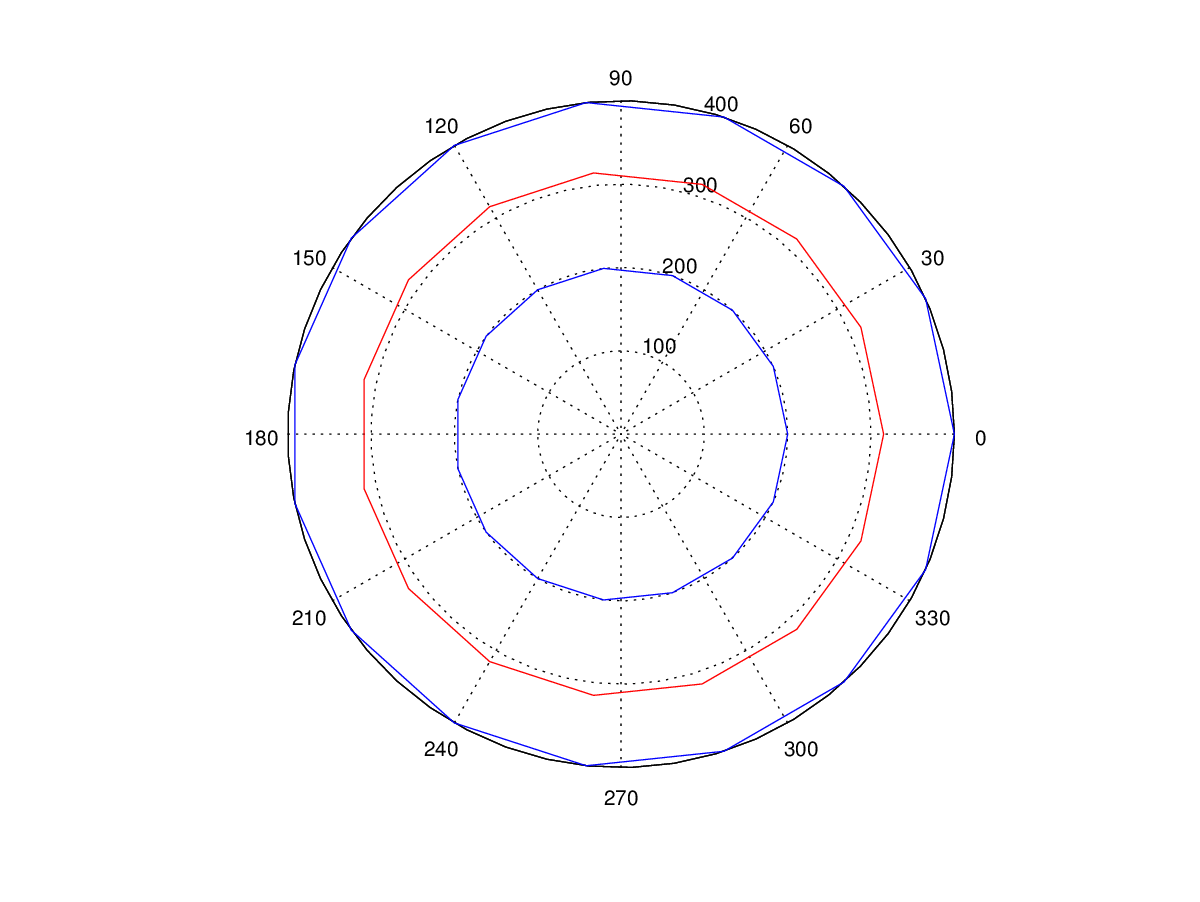
\includegraphics[scale=0.35]{experimentos1a_1b/evolucion_posicion_isoterma_temperatura/variacion_radios_angulos_se_reduce_diferencia_radial/test11_testord_001_inst_001_isomap.png}
		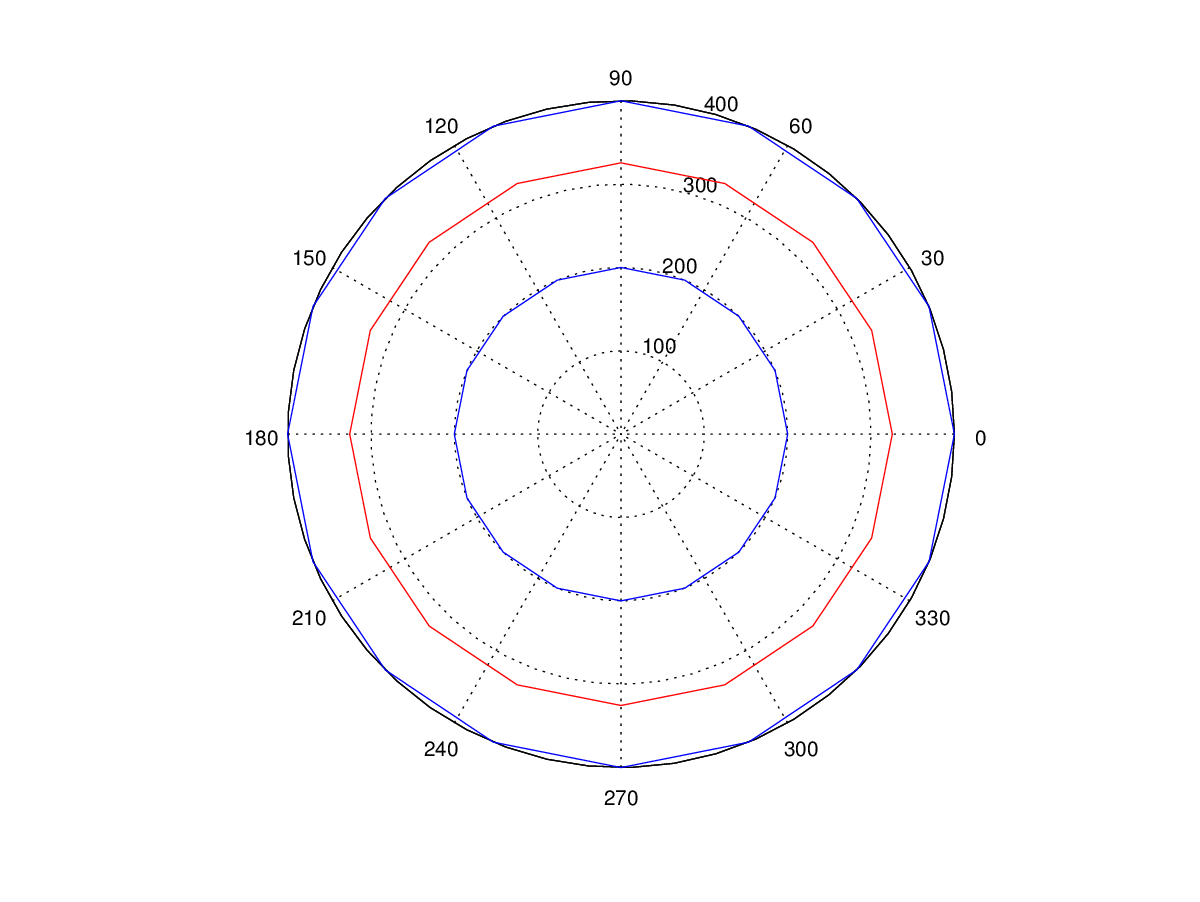
\includegraphics[scale=0.35]{experimentos1a_1b/evolucion_posicion_isoterma_temperatura/variacion_radios_angulos_se_reduce_diferencia_radial/test11_testord_002_inst_001_isomap.png}

	  	\textbf{Variación de la temperatura entre 59 y 60 radios, ángulos de discretización}\\
	  	\includegraphics[scale=0.35]{experimentos1a_1b/evolucion_posicion_isoterma_temperatura/variacion_radios_angulos_se_reduce_diferencia_radial/test11_testord_001_inst_001_heatmap.png}
		\includegraphics[scale=0.35]{experimentos1a_1b/evolucion_posicion_isoterma_temperatura/variacion_radios_angulos_se_reduce_diferencia_radial/test11_testord_002_inst_001_heatmap.png}

	  	\textbf{Variación de la estimación de la isoterma entre 15 y 16 radios, ángulos de discretización}\\
		\includegraphics[scale=0.35]{experimentos1a_1b/evolucion_posicion_isoterma_temperatura/variacion_radios_angulos_se_reduce_diferencia_radial/test11_testord_045_inst_001_isomap.png}
		\includegraphics[scale=0.35]{experimentos1a_1b/evolucion_posicion_isoterma_temperatura/variacion_radios_angulos_se_reduce_diferencia_radial/test11_testord_046_inst_001_isomap.png}

		\textbf{Variación de la temperatura entre 59 y 60 radios, ángulos de discretización}\\
	  	\includegraphics[scale=0.35]{experimentos1a_1b/evolucion_posicion_isoterma_temperatura/variacion_radios_angulos_se_reduce_diferencia_radial/test11_testord_045_inst_001_heatmap.png}
		\includegraphics[scale=0.35]{experimentos1a_1b/evolucion_posicion_isoterma_temperatura/variacion_radios_angulos_se_reduce_diferencia_radial/test11_testord_046_inst_001_heatmap.png}
\FloatBarrier
\vspace{0.5cm}

En este último ejemplo ocurren ambos fenomenos al mismo tiempo, hay una variación radial menor a medida que crecen los radios y la curva se suaviza al aumentar los ángulos.

\end{enumerate}

\vspace{0.5cm}

Efectivamente, podemos concluir que mientras más fina sea la discretización, se obtendrán resultados más \texttt{estables y confiables} acerca de la estimación. Uno de los motivos es porque habrá menos puntos para interpolar en la posición de la isoterma y el otro porque se tiene más informacion de la temperatura de la pared del horno.

\subsubsection{Estimación de estabilidad de la pared del horno}

Se presentarán a continuación los resultados de la estimacion de la estabilidad del horno. Para varios tipos de discretizaciones donde la cantidad de ángulos y radios son iguales, se evalua el cambio de posicion de la isoterma a medida que va aumentando la temperatura externa entre 100 y 300 grados, de a 2 grados por paso. Dado que las temperaturas son constantes, el máximo y el promedio coinciden como métricas de posicionamiento relativo de la isoterma.

\begin{figure}[h]
\centering

\includegraphics[scale=0.3]{experimentos1a_1b/evolucion_estimacion_seguridad_isoterma/variacion_25.png}
\includegraphics[scale=0.3]{experimentos1a_1b/evolucion_estimacion_seguridad_isoterma/variacion_50.png}	

\caption{Cantidad de radios y ángulos: 25(Izq) 50(Der)}
\end{figure}

\begin{figure}[h]
\centering

\includegraphics[scale=0.3]{experimentos1a_1b/evolucion_estimacion_seguridad_isoterma/variacion_75.png}
\includegraphics[scale=0.3]{experimentos1a_1b/evolucion_estimacion_seguridad_isoterma/variacion_100.png}	

\caption{Cantidad de radios y ángulos: 75(Izq) 100(Der)}
\end{figure}

\begin{figure}[h]
\centering

\includegraphics[scale=0.5]{experimentos1a_1b/evolucion_estimacion_seguridad_isoterma/variacion_125.png}

\caption{Cantidad de radios y ángulos: 125}
\end{figure}

\begin{figure}[h]
\centering

\includegraphics[scale=0.5]{experimentos1a_1b/evolucion_estimacion_seguridad_isoterma/variacion_30a_200r.png}
\caption{Cantidad de radios 200 - ángulos: 30}

\includegraphics[scale=0.5]{experimentos1a_1b/evolucion_estimacion_seguridad_isoterma/variacion_5a_500r.png}
\caption{Cantidad de radios 500 - ángulos: 5}
\end{figure}
\FloatBarrier

Los gráficos son un poco mas extraños de lo esperado. Se observa que, para cualquier discretizacion fija, al aumentar la temperatura externa, la isoterma tiende a acercarse a la pared externa. Esto es lo esperable, el método propuesto para determinar la seguridad de la isoterma consiste en fijar un umbral sobre la posicion relativa máxima o promedio. Lo que se observa como raro es la curva \texttt{dentada} a medida que crecen las temperaturas. Veamos además que estos \texttt{dientes} disminuyen su intensidad a medida que se van agregando radios a la discretizacion. 

\begin{proposition} 
	Bajo que las temperaturas internas y externas constantes, la posicion radial de la isoterma es la misma en todo ángulo.	
\end{proposition}

Dada esta última proposición, podemos hacer experimentos con muy pocos ángulos y muchos radios que nos den pauta de que ocurre con esos \texttt{dientes} en los gráficos. \\
Se puede observar en las figuras con 200 y 500 radios, que a medida que $m\to\infty$ , la curva se suaviza. Lo cual nos hace pensar, que la estimacion lineal de la isoterma esta generando esta distorsión.

\vspace{0.5cm}

Consideremos nuevamente $\hat{g_{\theta_i}}$: la función \textbf{discreta de aproximaciones} de temperatura de un ángulo i. A medida que las temperaturas aumentan linealmente, los 2 puntos $x$ y $x'$ que acotan la isoterma buscada en dicha función van aumentando tambien, generando que la estimacion del punto intermedio entre ellos decrezca. Creemos que cuando esos 2 puntos dejan se encerrar el valor buscado, es que se produce el \texttt{salto} en el gráfico.

\begin{proposition}
	El método de umbral de seguridad es inconsistente tomando la distancia máxima relativa o distancia promedio relativa a la pared exterior.
\end{proposition}

En los resultados anteriores y en el gráfico presentado en el primer experimento de ubicacion de la isoterma (convergencia radial de la isoterma). Se puede observar claramente, que trazando una recta horizontal en algún punto del eje Y, la determinación de colapso no es consistente. Es decir, existen $t_1 < t_2 < t_3$ temperaturas crecientes donde tanto la posicion máxima relativa o la posicion promedio relativa, indican peligro de colapso para $t_2$ pero no para $t_1$ ni $t_3$. Sin embargo, cuando $m\to\infty$ esto tiende a ser \texttt{menos inconsistente}.

\subsubsection{Análisis de la interpolacion lineal de la curva de temperatura}

Dados los resultados de la sección anterior, nos interesó saber un poco mas la forma de la funcion de temperatura sobre un ángulo fijo $\hat{g_{\theta_i}}$. 
Variamos un poco la cantidad de radios, y graficamos la función obtenida de los puntos de la discretización en una dirección fija y un fitteo lineal.
El resultado de los gráficos muestra que la temperatura no se disipa linealmente entre el interior y el exterior del horno. Dado que nosotros aproximamos linealmente la posicion radial de la isoterma 500 \textbf{entre los 2 puntos mas cercanos}, tendremos un error en cada \texttt{cambio de puntos} para la aproximacion.\\

Esto fortalece nuestra hipótesis de la sección anterior de que la forma de diente de sierra de los gráficos podía deberse a la interpolacion de algo no lineal, mediante una recta en puntos consecutivos.

\begin{figure}[h]
\centering
\includegraphics[scale=0.34]{funcion_temp_50_radios_ti_1500_te_102.png}
\includegraphics[scale=0.34]{funcion_temp_50_radios_ti_1500_te_202.png}
\caption{Distintas temperaturas externas - Cantidad de radios: 50}
\end{figure}
\FloatBarrier

\begin{figure}[h]
\centering
\includegraphics[scale=0.34]{funcion_temp_75_radios_ti_1500_te_102.png}
\includegraphics[scale=0.34]{funcion_temp_75_radios_ti_1500_te_202.png}
\caption{Distintas temperaturas externas - Cantidad de radios: 75}
\end{figure}
\FloatBarrier

\begin{figure}[h]
\centering
\includegraphics[scale=0.34]{funcion_temp_150_radios_ti_1500_te_102.png}
\includegraphics[scale=0.34]{funcion_temp_500_radios_ti_1500_te_102.png}
\caption{Cantidad de radios: 150(izq) , 500(der)}
\end{figure}
\FloatBarrier

\begin{figure}[h]
\centering
\includegraphics[scale=0.8]{efecto_interpolacion_lineal.png}
\caption{Esquema aproximado: Efecto interpolacion lineal entre puntos de algo no lineal}
\label{fig:aprox}
\end{figure}
\FloatBarrier

En la figura \ref{fig:aprox} se ve lo que podría estar ocurriendo al aproximar linealmente 2 puntos de una curva que realmente no es lineal. La recta entre dos puntos queda por encima de la curva real, luego, si se quiere hallar el $x$ tal que $g(x) = \alpha$ , la aproximación falla por un $\epsilon$ que depende de la concavidad de la curva respecto a la recta. A medida que se van agregando radios a la discretizacion, la distancia entre los puntos que se aproximan disminuye, disminuyendo el error cometido al estimar. 


\clearpage

%\section{Discusión}
%% TODO
Se incluira aqu un analisis de los resultados obtenidos en la seccion anterior (se analizara
su  validez,  coherencia,  etc.).   Deben  analizarse  como  mnimo  los tems  pedidos  en  el
enunciado.  No es aceptable decir que los resultados fueron los esperados", sin hacer
clara referencia a la teora a la cual se ajustan.  Ademas, se deben mencionar los resul-
tados interesantes y los casos patologicos" encontrados.


%\clearpage

\section{Conclusiones}
%!TEX root = informe.tex
\IEEEPARstart{A}{} lo largo de este trabajo atacamos el problema de generar frames artificiales para un video, intentando lograr que se ajusten al original hasta el punto -ideal- de que el ojo humano no detecte la diferencia con un video filmado en alta frecuencia.

Como primera conclusión al respecto podemos decir que no logramos dicho objetivo ideal: de nuestras observaciones descubrimos fácilmente que, al menos para los tres métodos implementados, los resultados ``no engañan a nadie''. Todos los métodos presentan o bien \emph{lag} o bien \emph{fantasmeo}, perturbando la sensación de fluidez y alterando el realismo percibido del video.

Más allá de ese análisis cualitativo, pudimos observar que atacar el problema de forma \emph{naïve} (el método que llamamos ``Vecino más cercano'') produce resultados con error matemático más reducido aunque visualmente pareciera ser el peor método, pudiendo obtenerse resultados visualmente más agradables con métodos más inteligentes como interpolación mediante poliniomios.

También concluimos que, visto como método de compresión, los resultados son pobres. En la actualidad existen métodos que, sin utilizar mucho más espacio, generan prácticamente nulos \emph{artifacts} y no pierden información de cuadros completos.
\clearpage

\section{Apéndice}
\subsection{Apéndice A: Enunciado}\label{enunciado}
  
\begin{centering}
\bf Laboratorio de M\'etodos Num\'ericos - Segundo Cuatrimestre 2015 \\
\bf Trabajo Pr\'actico N\'umero 1: Con 15 $\theta$s discretizo alto horno\ldots\\
\end{centering}

\vskip 25pt
\hrule
\vskip 11pt

{\bf Introducción}

Consideremos la secci\'on horizontal de un horno de acero cil\'indrico, como en la Figura 1. El sector A es la pared del horno, y el sector B es el horno propiamente dicho, en el cual se funde el acero a temperaturas elevadas. Tanto el borde externo como el borde interno de la pared forman c\'irculos. Suponemos que la temperatura del acero dentro del horno (o sea, dentro de B) es constante e igual a 1500$^{o}$C.

\medskip

Tenemos sensores ubicados en la parte externa del horno para medir la temperatura de la pared externa del mismo, que habitualmente se encuentra entre 50$^{o}$C y 200$^{o}$C. El problema que debemos resolver consiste en estimar la isoterma de 500$^{o}$C dentro de la pared del horno, para estimar la resistencia de la misma. Si esta isoterma est\'a demasiado cerca de la pared externa del horno, existe peligro de que la estructura externa de la pared colapse.


\begin{figure}[ht]
\begin{center}
\includegraphics[width=0.6\columnwidth]{img/Horno.png}
\caption{Secci\'on circular del horno}
\end{center}
\end{figure}



El objetivo del trabajo práctico es implementar un programa que calcule la isoterma solicitada, conociendo las dimensiones del horno y las mediciones de temperatura en la pared exterior.

{\bf El Modelo}

Sea $r_e \in \mathbb{R}$ el radio exterior de la pared y sea $r_i \in \mathbb{R}$ el radio interior de la pared. Llamemos $T(r,\theta)$ a la temperatura en el punto dado por las coordenadas polares $(r,\theta)$, siendo $r$ el radio y $\theta$ el \'angulo polar de dicho punto. En el estado estacionario, esta temperatura satisface la ecuaci\'on del calor:

\begin{equation}\label{calor}
\frac{\partial^2T(r,\theta)}{\partial r^2}+\frac{1}{r}\frac{\partial T(r,\theta)}{\partial r}+\frac{1}{r^2}\frac{\partial^2T(r,\theta)}{\partial \theta^2} = 0 
\end{equation}


Si llamamos $T_i \in \mathbb{R}$ a la temperatura en el interior del horno (sector B) y $T_e : [0,2\pi] \rightarrow \mathbb{R}$ a la funci\'on de temperatura en el borde exterior del horno (de modo tal que el punto $(r_e,\theta)$ tiene temperatura $T_e(\theta)$), entonces tenemos que

\begin{equation}
T(r,\theta) = T_i \;\;\;\;\;para\;todo\;punto\;(r,\theta)\;con\;r\leq r_i
\end{equation}
\begin{equation}
T(r_e,\theta) = T_e(\theta) \;\;\;\;\;\;para\;todo\;punto\;(r_e,\theta)
\end{equation}


El problema en derivadas parciales dado por la primera ecuaci\'on con las condiciones de contorno presentadas recientemente, permite encontrar la funci\'on $T$ de temperatura en el interior del horno (sector A), en funci\'on de los datos mencionados en esta secci\'on.

Para resolver este problema computacionalmente, discretizamos el dominio del problema (el sector A) en coordenadas polares. Consideramos una partici\'on $0 = \theta_0 < \theta_1 < ... < \theta_n = 2\pi$ en $n$ \'angulos discretos con $\theta_k-\theta_{k-1} = \Delta\theta$ para $k = 1,...,n$, y una partici\'on $r_i = r_0 < r_1 < ... < r_m = r_e$ en $m+1$ radios discretos con $r_j - r_{j-1} = \Delta r$ para $j = 1,...,m$.

\medskip

El problema ahora consiste en determinar el valor de la funci\'on $T$ en los puntos de la discretizaci\'on $(r_j,\theta_k)$ que se encuentren dentro del sector A. Llamemos $t_{jk} = T(r_j,\theta_k)$ al valor (desconocido) de la funci\'on $T$ en el punto $(r_j,\theta_k)$.

\medskip

Para encontrar estos valores, transformamos la ecuaci\'on (\ref{calor}) en un conjunto de ecuaciones lineales sobre las inc\'ognitas $t_{jk}$, evaluando (\ref{calor}) en todos los puntos de la discretizaci\'on que se encuentren dentro del sector A. Al hacer esta evaluaci\'on, aproximamos las derivadas parciales de $T$ en (\ref{calor}) por medio de las siguientes f\'ormulas de diferencias finitas:


\begin{equation}
\frac{\partial^2T(r,\theta)}{\partial r^2}(r_j,\theta_k) \cong \frac{t_{j-1,k}-2t_{jk}+t_{j+1,k}}{(\Delta r)^2}
\end{equation}

\begin{equation}
\frac{\partial T(r,\theta)}{\partial r}(r_j,\theta_k) \cong \frac{t_{j,k}-t_{j-1,k}}{\Delta r}
\end{equation}

\begin{equation}
\frac{\partial^2T(r,\theta)}{\partial \theta^2}(r_j,\theta_k) \cong \frac{t_{j,k-1}-2t_{jk}+t_{j,k+1}}{(\Delta \theta)^2}
\end{equation}



Es importante notar que los valores de las inc\'ognitas son conocidos para los puntos que se encuentran sobre el borde exterior de la pared, y para los puntos que se encuentren dentro del sector B. Al realizar este procedimiento, obtenemos un sistema de ecuaciones lineales que modela el problema discretizado. La resoluci\'on de este sistema permite obtener una aproximaci\'on de los valores de la funci\'on $T$ en los puntos de la discretizaci\'on.

{\bf Enunciado}

Se debe implementar un programa en \verb+C+ o \verb-C++- que tome como entrada los par\'ametros del problema ($r_i$, $r_e$, $m+1$,
$n$, valor de la isoterma buscada, $T_i$, $T_e(\theta)$) que calcule la temperatura dentro de la pared del horno utilizando el
modelo propuesto en la secci\'on anterior y que encuentre la isoterma buscada en funci\'on del resultado obtenido del
sistema de ecuaciones. El m\'etodo para determinar la posici\'on de la isoterma queda a libre elecci\'on de cada grupo y
debe ser explicado en detalle en el informe.

El programa debe formular el sistema obtenido a partir de las ecuaciones (1) - (6) y considerar dos m\'etodos posibles
para su resoluci\'on: mediante el algoritmo cl\'asico de Eliminaci\'on Gaussiana y la Factorizaci\'on LU. Finalmente, el
programa escribir\'a en un archivo la soluci\'on obtenida con el formato especificado en la siguiente secci\'on.

Como ya se ha visto en la materia, no es posible aplicar los m\'etodos propuestos para la resoluci\'on a cualquier
sistema de ecuaciones. Sin embargo, la matriz del sistema considerado en el presente trabajo cumple con ser diagonal dominante (no
estricto) y que, ordenando las variables y ecuaciones convenientemente, es posible armar un sistema de ecuaciones cuya matriz
posee la propiedad de ser \emph{banda}. Luego, se pide demostrar (o al menos dar un esquema de la demostraci\'on)
el siguiente resultado e incluirlo en el informe:

\begin{proposition}
Sea $A \in \mathbb{R}^{n \times n}$ la matriz obtenida para el sistema definido por (1)-(6). Demostrar que es posible
aplicar Eliminaci\'on Gaussiana sin pivoteo.\footnote{Sugerencia: Notar que la matriz es diagonal dominante (no
estrictamente) y analizar qué sucede al aplicar un paso de Eliminaci\'on Gaussiana con los elementos de una fila.} 
\end{proposition}

La soluci\'on del sistema de ecuaciones permitir\'a saber la temperatura en los puntos de la discretizaci\'on. Sin embargo,
nuestro inter\'es es calcular la isoterma 500, para poder determinar si la estructura se encuentra en peligro. Luego, se pide lo siguiente:
\begin{itemize}
\item Dada la soluci\'on del sistema de ecuaciones, proponer una forma de estimar en cada \'angulo de la discretizaci\'on la posici\'on de la 
isoterma 500.
\item En funci\'on de la aproximaci\'on de la isoterma, proponer una forma (o medida) a utilizar para evaluar la peligrosidad de la estructura
en funci\'on de la distancia a la pared externa del horno.
\end{itemize}


En funci\'on de la experimentaci\'on, se busca realizar dos estudios complementarios: por un lado, analizar c\'omo se comporta el sistema y, por otro, 
cu\'ales son los requerimientos computacionales de los m\'etodos. Se pide como m\'inimo realizar los siguientes experimentos:
\begin{enumerate}
\item Comportamiento del sistema.
\begin{itemize}
\item Considerar al menos dos instancias de prueba, generando distintas discretizaciones para cada una de ellas y
comparando la ubicaci\'on de la isoterma buscada respecto de la pared externa del horno. Se sugiere presentar gr\'aficos
de temperatura o curvas de nivel para los mismos, ya sea utilizando las herramientas provistas por la c\'atedra o
implementando sus propias herramientas de graficaci\'on. 
\item Estudiar la proximidad de la isoterma buscada respecto de la pared exterior del horno en funci\'on de distintas 
granularidades de discretizaci\'on y las condiciones de borde. 
\end{itemize}
\item Evaluaci\'on de los m\'etodos.
\begin{itemize}
\item Analizar el tiempo de c\'omputo requerido para obtener la soluci\'on del sistema en funci\'on de la granularidad de 
la discretizaci\'on. Se sugiere presentar los resultados mediante gr\'aficos de tiempo de c\'omputo en funci\'on de alguna 
de las variables del problema.
\item Considerar un escenario similar al propuesto en el experimento 1. pero donde las condiciones de borde (i.e., $T_i$ y $T_e(\theta)$)
cambian en distintos instantes de tiempo. En este caso, buscamos obtener la secuencia de estados de la temperatura en
la pared del horno, y la respectiva ubicaci\'on de la isoterma especificada. Para ello, se considera una secuencia de $ninst$
vectores con las condiciones de borde, y las temperaturas en cada estado es la soluci\'on del correspondiente sistema de
ecuaciones. Se pide formular al menos un experimento de este tipo, aplicar los m\'etodos de resoluci\'on propuestos de
forma conveniente y compararlos en t\'erminos de tiempo total de c\'omputo requerido para distintos valores de $ninst$.
\end{itemize}
\end{enumerate}

De manera opcional, aquellos grupos que quieran ir un poco m\'as all\'a pueden considerar trabajar y desarrollar alguno(s) 
de los siguientes puntos extra:
\begin{enumerate}
\item Notar que el sistema resultante tiene estructura \emph{banda}. Proponer una estructura para aprovechar este hecho en t\'erminos de la
\emph{complejidad espacial} y como se adaptar\'ian los algoritmos de Eliminaci\'on Gaussiana y Factorizaci\'on LU para reducir la
cantidad de operaciones a realizar.
\item Implementar dicha estructura y las adaptaciones necesarias para el algoritmo de Eliminaci\'on Gaussiana.
\item Implementar dicha estructura y las adaptaciones necesarias para el algoritmo de Factorizaci\'on LU. 
\end{enumerate}

Finalmente, se deber\'a presentar un informe que incluya una descripci\'on detallada de los m\'etodos implementados y
las decisiones tomadas, el m\'etodo propuesto para el c\'alculo de la isoterma buscada y los experimentos realizados,
junto con el correspondiente an\'alisis y siguiendo las pautas definidas en el archivo \verb+pautas.pdf+.

{\bf Programa y formato de archivos}

Se deber\'an entregar los archivos fuentes que contengan la resoluci\'on del trabajo pr\'actico. El ejecutable tomar\'a
tres par\'ametros por l\'inea de comando, que ser\'an el archivo de entrada, el archivo de salida, y el m\'etodo a
ejectutar (0 EG, 1 LU).

El archivo de entrada tendr\'a la siguiente estructura:
\begin{itemize}
\item La primera l\'inea contendr\'a los valores $r_i$, $r_e$, $m+1$, $n$, $iso$, $ninst$, donde $iso$ representa el
valor de la isoterma buscada y $ninst$ es la cantidad de instancias del problema a resolver para los par\'ametros dados.
\item A continuaci\'on, el archivo contendr\'a $ninst$ l\'ineas, cada una de ellas con $2n$ valores, los primeros $n$ indicando los
valores de la temperatura en la pared interna, i.e., $T_i(\theta_0),T_i(\theta_1),\dots,T_i(\theta_{n-1})$, seguidos de $n$ valores
de la temperatura en la pared externa, i.e., $T_e(\theta_0)$,$T_e(\theta_1)$,$\dots$,$T_e(\theta_{n-1})$.
\end{itemize}

El archivo de salida obligatorio tendr\'a el vector soluci\'on del sistema reportando una componente del mismo por
l\'inea. En caso de $ninst > 1$, los vectores ser\'an reportados uno debajo del otro.

Junto con el presente enunciado, se adjunta una serie de scripts hechos en \verb+python+ y un conjunto instancias de
test que deber\'an ser utilizados para la compilaci\'on y un testeo b\'asico de la implementaci\'on. Se recomienda leer
el archivo \verb+README.txt+ con el detalle sobre su utilizaci\'on.

{\bf \underline{Fechas de entrega}}
\begin{itemize}
\item \emph{Formato Electr\'onico:} Jueves 3 de Septiembre de 2015, hasta las 23:59 hs, enviando el trabajo (informe +
c\'odigo) a la direcci\'on \verb+metnum.lab@gmail.com+. El subject del email debe comenzar con el texto \verb+[TP1]+
seguido de la lista de apellidos de los integrantes del grupo.
\item \emph{Formato f\'isico:} Viernes 4 de Septiembre de 2015, de 17:30 a 18:00 hs.
\end{itemize}

\noindent \textbf{Importante:} El horario es estricto. Los correos recibidos despu\'es de la hora indicada ser\'an
considerados re-entrega. Los grupos deben ser de 3 o 4 personas, sin excepci\'on. Es indispensable que los trabajos
pasen satisfactoriamente los casos de test provistos por la c\'atedra.

\clearpage
\subsection{Apéndice B: Código relevante}
  \lstinputlisting[language=C++, caption=Eliminacion gaussiana]{gaussiana.ctex}
\lstinputlisting[language=C++, caption=Factorizacion LU]{lu.ctex}

%\section{Referencias}
\end{document}
